\documentclass[12pt]{article}
\setlength{\headheight}{35pt} 

%----------------------------------------------------------
% Packages
%----------------------------------------------------------
\usepackage[vmargin=1.18in,hmargin=1.1in]{geometry}				% page layout
\usepackage{amssymb,amsfonts,amsthm,mathtools,bm,bbm,mathrsfs} 	% math fonts/symbols
\usepackage[dvipsnames]{xcolor} 								% for \textcolor
\usepackage[colorlinks, linkcolor = blue, citecolor = blue, urlcolor = blue]{hyperref} 								% for hyperlinks 
\usepackage{graphicx} 											% for \includegraphics
\usepackage{caption} 											% for figure and table captions
\usepackage{verbatim}
\usepackage[misc]{ifsym} 										% for \Letter
\usepackage[ruled, linesnumbered]{algorithm2e} 					% for algorithm box
\usepackage{layouts} % to get information about document layout
\usepackage[uniquename=false, 
			uniquelist = false, 
			url = false, 
			doi = false, 
			isbn = false, 
			natbib = true, 
			backend = bibtex, 
			style = authoryear, 
			maxbibnames = 5]{biblatex} 							% for citations and bibliography
% \RequirePackage{amsthm,amsmath,amsfonts,amssymb,mathtools,bm,bbm,mathrsfs}  % typesetting                                    % author-year citations
% \RequirePackage[colorlinks,citecolor=blue,urlcolor=blue]{hyperref}          % coloring bibliography citations and linked URLs                                        
% \RequirePackage{verbatim}
% \RequirePackage[ruled, linesnumbered]{algorithm2e} 					        % for algorithm box
\usepackage{booktabs} % to make book table
\usepackage{multirow} % to create table with multirow
\usepackage[noend]{algpseudocode}
\usepackage{subcaption}
\usepackage{multirow}

\geometry{a4paper,scale=0.75}

\newenvironment{breakablealgorithm}
{% \begin{breakablealgorithm}
	\begin{center}
		\refstepcounter{algorithm}% New algorithm
		\hrule height.8pt depth0pt \kern2pt% \@fs@pre for \@fs@ruled
		\renewcommand{\caption}[2][\relax]{% Make a new \caption
			{\raggedright\textbf{\ALG@name~\thealgorithm} ##2\par}%
			\ifx\relax##1\relax % #1 is \relax
			\addcontentsline{loa}{algorithm}{\protect\numberline{\thealgorithm}##2}%
			\else % #1 is not \relax
			\addcontentsline{loa}{algorithm}{\protect\numberline{\thealgorithm}##1}%
			\fi
			\kern2pt\hrule\kern2pt
		}
	}{% \end{breakablealgorithm}
		\kern2pt\hrule\relax% \@fs@post for \@fs@ruled
	\end{center}
}
\makeatother


\newcommand{\zn}[1]{\textcolor{purple}{[ZN: #1]}}
\newcommand{\ek}[1]{\textcolor{red}{[EK: #1]}}
\newcommand{\jrc}[1]{\textcolor{blue}{[JRC: #1]}}

\newtheorem{assumption}{Assumption}
\newtheorem{theorem}{Theorem}
\newtheorem{corollary}{Corollary}
\newtheorem{lemma}{Lemma}
\newtheorem{proposition}{Proposition}
\newtheorem{definition}{Definition}
\theoremstyle{definition}
\newtheorem{example}{Example}
\newtheorem{remark}{Remark}
\newcommand{\indep}{\perp \!\!\! \perp}


%%%%%%%%%%%%%%%%%%%%%%%%%%%%%%

\def\X{\bm{X}}
\def\mP{\mathbb{P}}
\def\A{\bm{A}}
\def\P{\mathbb{P}}
\def\iid{\mathrm{iid}}
\def\H{\mathcal{H}}
\def\Hk{\mathcal{H}_k}
\def\tht{\bm{\theta}}
\def\gama{\bm{\gamma}}
\def\Del{\bm{\Delta}}
\def\sgn{\mathrm{sgn}}
\def\P{\mathbb{P}}


%----------------------------------------------------------
% Generic macros
%----------------------------------------------------------
\newcommand{\E}{\mathbb E}								% expectation
\newcommand{\V}{\mathrm{Var}}							% variance
\renewcommand{\P}{\mathbb{P}}							% probability
\newcommand{\Q}{\mathbb{Q}}								% quantile
\newcommand{\R}{\mathbb{R}}								% reals
\newcommand{\Z}{\mathbb{Z}}								% integers
\newcommand{\N}{\mathbb{N}}								% naturals
\newcommand{\indicator}{\mathbbm 1}						% indicator
\newcommand{\norm}[1]{\left\lVert{#1}\right\rVert}		% norm
\newcommand{\independent}{{\perp \! \! \! \perp}}		% independent
\newcommand{\iidsim}{\stackrel{\mathrm{i.i.d.}}{\sim}} 	% i.i.d. distributed
\newcommand{\indsim}{\stackrel{\mathrm{ind}}{\sim}}		% independently distributed
\newcommand{\expit}{\mathrm{expit}}                 	% link function for logistic model
\newcommand{\convp}{\overset{\mathbb{P}}{\rightarrow}}             % convergence in probability
\newcommand{\convd}{\overset d \rightarrow}             % convergence in distribution
\newcommand{\convas}{\overset {a.s.} \rightarrow}       % convergence almost surely
\newcommand{\argmin}[1]{\underset{#1}{\arg \min}}       % arg min
\newcommand{\argmax}[1]{\underset{#1}{\arg \max}}       % arg max

%----------------------------------------------------------
% Paper-specific macros
%----------------------------------------------------------
\newcommand{\prx}{\bm X}								% population random X
\newcommand{\srx}{X}									% sample random X
\newcommand{\prz}{\bm Z}								% population random Z
\newcommand{\srz}{Z}									% sample random Z 
\newcommand{\prxk}{{{\widetilde{\bm X}}}}      			% population random resampled X
\newcommand{\seta}{s^{2}(\eta_0)}
\newcommand{\srxk}{\widetilde X}						% sample random resampled X
\newcommand{\pry}{{\bm Y}}								% population random Y
\newcommand{\pru}{{\bm U}}								% population random U
\newcommand{\sry}{Y}									% sample random Y 
\newcommand{\peps}{\bm \epsilon}						% population epsilon
\newcommand{\seps}{\epsilon}							% sample epsilon
\newcommand{\smu}{\mu}									% sample mu
\newcommand{\pmu}{\bm \mu}								% population mu
\newcommand{\law}{\mathcal L}							% law of (X,Y,Z)
\newcommand{\nulllaws}{\mathscr L^0}					% collection of null distributions
\newcommand{\regclass}{\mathscr R}					    % collection of distributions with regularity
\newcommand{\lawhat}{\widehat{\mathcal L}}				% estimated law of (X,Y,Z)
\newcommand{\CRT}{\textnormal{CRT}}             		% CRT
\newcommand{\dCRT}{\textnormal{dCRT}} 					% dCRT
\newcommand{\odCRT}{\textnormal{odCRT}} 					% dCRT
\newcommand{\GCM}{\textnormal{GCM}}						% GCM
\newcommand{\oGCM}{\textnormal{oGCM}}						% GCM
\newcommand{\dCRThat}{\widehat{\textnormal{dCRT}}}		% dCRT-hat
\newcommand{\MXtwohat}{\widehat{\textnormal{MX(2)}}}		% dCRT-hat
\newcommand{\ndCRThat}{\textnormal{ndCRT}}	% normalized dCRT-hat
\newcommand{\CRThat}{\widehat{\textnormal{CRT}}}		% CRT-hat
\renewcommand{\H}{\mathcal H}		 					% Hilbert subspace
\newcommand{\MXtwo}{\textnormal{MX(2)}}                 % MX(2)
\newcommand{\convdp}{\overset {d,p} \longrightarrow}    % conditional convergence in distribution
\newcommand{\convpp}{\overset {p,p} \longrightarrow}    % conditional convergence in probability
\newcommand{\spacrt}{\textnormal{spaCRT}}               % spaCRT
\newcommand{\aux}{\textnormal{aux}}               % auxiliary test
\newcommand{\asy}{\textnormal{asy}}              % asymptotic test
%----------------------------------------------------------
% Other macros
%----------------------------------------------------------
\let\oldnl\nl% Store \nl in \oldnl
\newcommand{\nonl}{\renewcommand{\nl}{\let\nl\oldnl}} % Remove line number for one line of alg

\addbibresource{spacrt.bib}
% \bibliography{spacrt.bib}


%%%%%%%%%%%%%%%%%%%%%%%%%%%%%%%%%%%%%%%%%%
\title{Computationally efficient and statistically accurate conditional independence testing with spaCRT}

\begin{document}

\author{Ziang Niu, Jyotishka Ray Choudhury, Eugene Katsevich}
\maketitle


\begin{abstract}
  We introduce the saddlepoint approximation-based conditional randomization test (spaCRT), a novel conditional independence test that effectively balances statistical accuracy and computational efficiency, inspired by applications to single-cell CRISPR screens. Resampling-based methods like the distilled conditional randomization test (dCRT) offer statistical precision but at a high computational cost. The spaCRT leverages a saddlepoint approximation to the resampling distribution of the dCRT test statistic, achieving very similar finite-sample statistical performance with significantly reduced computational demands. We prove that the spaCRT $p$-value approximates the dCRT $p$-value with vanishing relative error, and that these two tests are asymptotically equivalent. The validity of $\spacrt$ is assessed with modern regression techniques applied such as lasso and kernel ridge regression. Through extensive simulations and real data analysis, we demonstrate that the spaCRT controls Type-I error and maintains high power, outperforming other asymptotic and resampling-based tests. Our method is particularly well-suited for data with low signal-to-noise ratio and large scale like single-cell CRISPR screen analyses, facilitating the efficient and accurate assessment of perturbation-gene associations.
\end{abstract}

\section{Introduction} \label{sec:introduction}

Conditional independence testing is a fundamental problem in statistics. Given the joint distribution $(\prx, \pry, \prz) \sim \law_n$ (potentially depending on sample size $n$), the statistical task is to test the null hypothesis 
\begin{equation}\label{eq:conditional-independent-null}
H_0: \prx \indep \pry \mid \prz. 
\end{equation}
In the language of causal inference \citep{imbens2015causal}, $\prx$ is often interpreted as a treatment variable, $\pry$ as an outcome variable, and $\prz$ as a set of covariates. The null hypothesis $H_0$ states that the treatment has no effect on the outcome, given the covariates. Suppose the independent and identically distributed observations $(\srx_{in}, \sry_{in}, \srz_{in}) \iidsim \law_n$ are collected for subject $i = 1, \dots, n$. We denote these observations collectively as $\srx \in \R^n$, $\sry \in \R^n$, $\srz \in \R^{n \times d}$.

\subsection{Challenges: low signal-to-noise ratio and large scale data} \label{sec:statistical-computational-challenges}

One particular challenge arises in modern applications involving testing conditional independence null \eqref{eq:conditional-independent-null}, is the low signal-to-noise (SNR) ratio in the data. Such low SNR can arise from high sparsity (i.e. excessive zeros) in the observed data $X$ and $Y$ and also the potential heavy tail behavior of these observations. In fact, the issue of sparsity is ubiquitous in the analysis of genomic data, especially in the single-cell resolution level. Moreover, the sparsity is not the single issue involved and the large scale in such data is another barrier further precluding the application of sophisticated yet computationally intensive statistical methods. We discuss one concrete example originating from single-cell CRISPR screens analysis.

One of the biological objectives in single-cell CRISPR screens \citep{Dixit2016,Adamson2016,Jaitin2016,Datlinger2017} is to understand \textit{regulatory elements}, segments of DNA whose role is to control the expressions of one or more nearby genes. To address this question, single-cell CRISPR screens are designed to subject a population of cells to a large number of \textit{CRISPR perturbations}, each of which inhibits the functioning of a specific regulatory element. Each cell receives several of these perturbations (treatment indicator $\prx\in\{0,1\}$), and the expression of each gene in each cell (count-based outcome $\pry\in\mathbb{N}$) is measured by single-cell RNA-sequencing. The statistical analysis task is to determine, for each CRISPR perturbation and gene of interest, whether cells with the perturbation have different gene expression levels compared to cells without the perturbation, subject to some collected technical covariate $\prz$ such as library size and batch effect. The challenges arise in two-fold: 
\paragraph{Sparsity in perturbations $X$ and gene expression $Y$:}

The excessive sparsity in the treatment indicator of $\srx$, because of the pooling nature of large scale perturbations, and relatively small gene expression count $\sry$, because of single-cell resolution and thus low coverage in RNA sequencing, can lead to a challenge of low effective sample size. Such challenge manifests itself when applying tests based on central limit theorem, in the infalted Type-I error rates \citep{Barry2024}.

\paragraph{Large scale in cells and tests:}

Sample size (number of cells) in such experiments can be as high as hundres of thousands. Moreover, computation challenge can be even more pronounced when considering a large number of hypotheses. This is usually the practice due to the screening nature of such experiments and thus excludes the possibility of direct application of method like resampling-based test procedures despite they are able to produce better calibrated $p$-values under the low effect sample size setup. As a concrete example on the scale of experiments, \citet{Gasperini2019a} tested about 90,000 perturbation-gene pairs with over $200,000$ cells. 

The double facets of statistical and computational challenges can also be found in genome-wide association studies (GWAS) even though the source of low effective sample size is different. We postpone the discussion of this example to Section~\ref{sec:simulation}. Certainly, the  challenges of applying the conditional independence test to modern data analysis can go beyond the low SNR and large scale. In fact, \citep{Shah2018} proved that the conditional independence test \eqref{eq:conditional-independent-null} is a fundamentally hard problem in the sense that there is no single test that can control Type-I error and simultaneously have nontrivial power against any alternative without further assumptions. 

\subsection{Relevant literature}

Resampling-based test procedures are particuarly suitable for analyzing data with low effective size due to their desirable finite-sample performance, but computation is the main challenge. In fact, in the example of \citet{Gasperini2019a}, given the multiplicity correction required for such a large number of tests, $p$-values need to be accurate to about seven decimal places to have a chance at significance (assuming a Bonferroni correction at level $\alpha = 0.05$). Then obtaining accurate $p$-values for each test requires about a million resamples per $p$-value, for a total of about $10^{12}$ resamples across all perturbation-gene pairs tested. In contrast, applying asymptotic tests can result in inflated Type-I error rates in low SNR setup while being much more computationally efficient. 

To resolve the dilemma between statistical accuracy and computational efficiency, a number of statistical testing or approximation procedures have been proposed. We divide the discussion of these literatures into two categories: resampling-based and resampling-free procedures. Our discussion will incoporate but go beyond the conditional independence test.

\paragraph{Resampling-based procedures.}


Resampling-based procedures have been accelerated using adaptive resampling schemes, which adjust the number of resamples drawn based on the data \citep{Besag1991,Gandy2009,Gandy2014,Gandy2016,Gandy2017a,Fischer2024a,Fischer2024}. Such procedures are applicable to arbitrary resampling schemes and test statistics, at the cost of some resampling. On a more applied side, to circumvent the computational barrier of resampling, \citet{Ge2012,Winkler2016} proposed heuristic methods to fit parametric curves on the resampled distributions so that the number of resampling can be kept in a relatively small scale used to learn the curves. \citep{Katsevich2020c} proposed to apply the $\dCRT$ \citep{Liu2022a}, which is an accelerated variant of the resampling-based \textit{conditional randomization test} (CRT; \cite{CetL16}) in the context of single-cell CRISPR screens, and applied the similar parametric curve fitting approach to the resampling distribution of $\dCRT$. 

\paragraph{Resampling-free procedures.}

A large class of methods in this category are based on finer asymptotic expansion techniques. For example, classical \textit{Edgeworth expansion} has been applied to study the null distribution of test statistics \citep{hall2013bootstrap,bentkus1997edgeworth,Bickel1974} to improve upon naive normal approximation. However, the Edgeworth expansion may suffer from accuracy when it comes to the tail area of the statistic distribution. In particular, Chapter 5 in \citet{hall2013bootstrap} showed the lack of relative error for Edgeworth expansion estimate, posing a challenge when small $p$-values are present. \textit{Saddlepoint approximation} (SPA, \citet{Daniels1954,Lugannani1980}) is another classical technique to obtain highly accurate approximations to densities and tail probabilities for quantities that can be expressed as sample averages. In particular, a desirable property of SPA is its relative error guarantee \citep{Butler2007,Kolassa2006}. SPAs have been proposed to approximate resampling distributions of classical resampling-based procedures, like permutation tests \citep{Robinson1982} and the bootstrap \citep{Hinkley1988}. Apart from these asymptotic approximations, exact computation of $p$-value based on the resampled distribution is possible for certain case. In the same paper where the $\dCRT$ was introduced \citep{Liu2022a}, a resampling-free approximation to this procedure was proposed based on a quantile transformation to a normal distribution. However, these authors acknowledged that this approach is primarily useful for continuously distributed $\prx$, and that it incurs a substantial power loss for discrete $\prx$, the setting that will be focused on in the present work. 

With these dense literatures discussed, reconciling the statistical accuracy and computational efficiency remains unresolved and open in the context of conditional independence testing \eqref{eq:conditional-independent-null}. 

\subsection{Our contributions}

In this paper, we propose a new method, the \textit{saddlepoint approximation-based conditional randomization test} ($\spacrt$). $\spacrt$ is a \textit{resampling-free} conditional independence testing procedure, which reconciles the statistical accuracy of the $\dCRT$ with the computational efficiency of asymptotic methods. The key idea is to approximate the distribution of the resampled test statistic in the $\dCRT$ using a saddlepoint approximation. Concretely, we make the following contributions:
\begin{enumerate}
  \item \textbf{Establish general approximation accuracy of $\spacrt$:}
  In Section~\ref{sec:general_results}, we prove the general theoretical results of approximation accuracy of $\spacrt$ in terms of the relative error of $p$-values and the test is then shown to be asymptotically equivalent to $\dCRT$ under mild regularity conditions. Therefore, $\spacrt$ inherits disrable properties of $\dCRT$ allowing general regression methods to learn $\E[\prx|\prz]$ and $\E[\pry|\prz]$.
  \item \textbf{Investigate validity of $\spacrt$ with modern regression techniques:} 
  Building on the general results, we show in Section~\ref{sec:case_study} that $\spacrt$ is valid under a wide range of regression techniques, encompassing generalized linear models, high-dimensional regression and nonparametric machine learning regression. The conditions for the accurate approximation of $\spacrt$ towards $\dCRT$ is no more stringent than consistency assumptions for the regression estimators.
  \item \textbf{Explore superior performance in genetics and genomics applications:} In Section~\ref{sec:simulation}, we demonstrate the superior finite-sample performance of $\spacrt$ in the simulation setups with sparse outcomes, which are motivated by GWAS and single-cell CRISPR screens. In Section~\ref{sec:real_data}, we apply $\spacrt$ to a single-cell CRISPR screens analysis \citep{Gasperini2019a} and show that $\spacrt$ is able to control Type-I error and maintain high power while requiring similar computational resources to the asymptotic tests.
  \item \textbf{Expand the applicability of SPA in modern statistics:} To the best of our knowledge, $\spacrt$ is the first application of SPA to a conditional independence test. One of the aims of this paper is to draw the attention of the statistical community to the potential of SPA in modern statistics. Its analytic nature makes SPA particularly well-suited for large-scale data analysis.
\end{enumerate} 

Code to reproduce these analyses is available at \href{https://github.com/Katsevich-Lab/spacrt-manuscript}{github.com/Katsevich-Lab/spacrt-manuscript}. 

\subsection{Notation}


Define $\sgn(x)$ as the sign of $x$, i.e. $\sgn(x)=1$ if $x>0$, $-1$ if $x<0$ and $0$ otherwise. For an infinitely differentiable function $f:\mathcal{X}\subset\mathbb{R}\mapsto\mathbb{R}$, define $f^{(r)}$ to be its $r$-th derivative. Define $f',f''$ as the first and second derivative of $f$ respectively. Denote $[n]$ for any $n\in\mathbb{N}_+$ as $\{1,\ldots,n\}$. Define $\expit(x)\equiv 1/ (1+\exp(-x))$. Define $\E_{\law_n}[\cdot\mid\mathcal{F}_n],\E_{\lawhat_n}[\cdot\mid\mathcal{F}_n]$ as the conditional expectations under law $\law_n$ and its estimate $\lawhat_n$ respectively. Similarly, we define $\V_{\law_n}[\cdot\mid\mathcal{F}_n]$ and $\V_{\lawhat_n}[\cdot\mid\mathcal{F}_n]$ as the conditional variance counterpart. We use the following standard notations regarding the asymptotic properties of a sequence of random variables $X_n$:
\begin{align*}
  &X_n = O_{\P}(1) &&\text{ if for each } \delta > 0 \text{ there is an } M > 0 \text{ s.t. } \limsup_{n \rightarrow \infty}\P[|X_n| > M] < \delta; \\
  &X_n = \Omega_{\P}(1) &&\text{ if for each } \delta > 0 \text{ there is an } \eta > 0 \text{ s.t. } \limsup_{n \rightarrow \infty}\P[|X_n| < \eta] < \delta;\\
  &X_n = o_{\P}(1) &&\text{ if } \P[|X_n| > \eta] \rightarrow 0 \text{ for all } \eta > 0.
\end{align*}
We use $a_n\sim b_n$ if $0<\liminf_{n\rightarrow\infty}|a_n/b_n|\leq\limsup_{n\rightarrow\infty}|a_n/b_n|<\infty$ and $a_n=o(b_n)$ if $\limsup_{n\rightarrow\infty}|a_n/b_n|\rightarrow0$. 

\section{A dilemma between $\dCRT$ and $\GCM$}\label{sec:finite_sample}

Before introducing the $\spacrt$, we first discuss the successful application of the $\dCRT$ in achieving better Type-I error control compared to its asymptotic counterpart, the \textit{generalized covariance measure} (GCM) test. However, the success in statistical performance builds on the computationally heavy resampling procedure. 

\subsection{Background: $\dCRT$ and $\GCM$ test}\label{sec:background}

The dCRT procedure, as proposed by \citet{Liu2022a}, is designed under the \textit{model-X assumption} that $\law_n(\prx \mid \prz)$ is known \citep{CetL16}. However, this procedure is usually deployed in practice by learning this conditional distribution in-sample. In a prior work, we established the statistical properties of the dCRT with $\law_n(\prx \mid \prz)$ estimated in sample \citep{Niu2022a}. In this paper, we will refer to the latter procedure as the $\dCRT$, allowing a minor abuse of terminology. Furthermore, we consider the special but still fairly general case when 
\begin{equation}
\law_n(\prx \mid \prz) = f(\prx \mid \theta_{n,x}(\prz)), 
\end{equation}
where $f(x|\theta)$ is an exponential family with natural parameter $\theta$, natural parameter space $\R$, and log-partition function $A$:
\begin{align}\label{eq:NEF}
f(x|\theta)=\exp(\theta x -A(\theta))h(x).
\end{align}
This is not a restrictive assumption, since we allow the function $\theta_{n,x}(\prz)$ to be arbitrary. Given this setup, consider estimating the functions $\theta_{n,x}(\prz)$ and $\mu_{n,y}(\prz) \equiv \E_{\law_n}[\pry \mid \prz]$ by $\widehat{\theta}_{n,x}(\prz)$ and $\widehat \mu_{n,y}(\prz)$, respectively (we assume throughout that $\pry$ is integrable, so that $\mu_{n,y}$ is well-defined). The learning procedures for these quantities can be arbitrary. The choices include but are not limited to parametric, non-parametric and high-dimensional regression methods. Setting $\widehat \mu_{n,x}(\prz) \equiv A'(\widehat{\theta}_{n,x}(\prz))$, we arrive at the test statistic 
\begin{align}\label{eq:dCRThat}
	T_n^{\dCRT}(X,Y,Z)
  =\frac{1}{n}\sum_{i=1}^{n}(\srx_{in}-\widehat\mu_{n,x}(\srz_{in}))(\sry_{in}-\widehat{\mu}_{n,y}(\srz_{in})).
\end{align}
The $\dCRT$ is obtained by comparing $T_n^{\dCRT}(\srx, \sry, \srz)$ to a null distribution obtained by resampling $\srx_{in} \mid \srz_{in}$ based on the estimated distribution $f(\cdot \mid \widehat \theta_{n,x}(Z_{in})).$ This procedure is summarized in Algorithm \ref{alg:dcrt-hat}. 

\begin{center}
	\begin{minipage}{\linewidth}
		\begin{algorithm}[H]
			\nonl  \textbf{Input:}  Data $(\srx,\sry,\srz)$, number of randomizations $M$. \\
			Learn $\widehat{\theta}_{n,x}(\cdot)$ and $\widehat \mu_{n,x}(\cdot)$ based on $(\srx, \srz)$; learn $\widehat{\mu}_{n,y}(\cdot)$ based on $(\sry, \srz)$\;
			Compute $T_n^{\dCRT}(\srx, \sry, \srz)$ as in \eqref{eq:dCRThat}\;
			\For{$m = 1, 2, \dots, M$}{
				Sample $\srxk^{(m)}|\srx, \sry, \srz \sim \prod_{i = 1}^n f(\cdot\mid\widehat{\theta}_{n,x}(\srz_{in}))$ and compute 
				\begin{equation}
					T_n^{\dCRT}(\srxk^{(m)}, \srx, \sry, \srz) \equiv \frac{1}{n}\sum_{i = 1}^n (\srxk^{(m)}_{in} - \widehat \mu_{n,x}(\srz_{in}))(\sry_{in} - \widehat \mu_{n,y}(\srz_{in})); \label{eq:resampled-dcrt-def}
				\end{equation}
			}
			\nonl \textbf{Output:} $\dCRT$ $p$-value $\frac{1}{M+1} (1+ \sum_{m=1}^M\indicator\{T_n^{\dCRT}(\srxk^{(m)}, \srx, \sry, \srz) \geq T_n^{\dCRT}(\srx, \sry, \srz)\}).$
			\caption{\bf $\dCRT$ procedure with exponential family for $\law_n(\prx \mid \prz)$}
			\label{alg:dcrt-hat}
		\end{algorithm}
	\end{minipage}
\end{center}

$\dCRT$ is a resampling-based procedure that can be computationally challenging when the sample size is moderate to large. An alternative test procedure is instead of using the resampling to construct $p$-value, one can use the normal approximation to the test statistic $T_n^{\dCRT}(\srx, \sry, \srz)$ \eqref{eq:dCRThat} under null and construct a $p$-value based on the cutoff of the standard normal distribution after properly normalizing the standard deviation estimate. This is the so-called GCM test \citep{Shah2018}. Building on the same test statistic (except for extra normalization), $\GCM$ also allows flexible modeling choices on estimators $\widehat{\mu}_{n,x}(\cdot)$ and $\widehat{\mu}_{n,y}(\cdot)$. In fact, it has been proved in \citet{Shah2018} that $\GCM$ enjoys the so-called double robustness property: as long as both estimators $\widehat\mu_{n,x}(\cdot)$ and $\widehat{\mu}_{n,y}(\cdot)$ are consistent and converge to the true conditional expectations at rate faster than $n^{-1/4}$, the validity of the test can be guaranteed \citep[Theorem 6]{Shah2018}. 

Proved in \citet{Niu2022a}, the $\dCRT$ is asymptotically equivalent to $\GCM$ under mild conditions. Thus $\dCRT$ inherits the doubly robust statistical property from $\GCM$. One important difference is $\dCRT$ relies on resampling to construct the $p$-value, while $\GCM$ relies on the asymptotic normal approximation. This difference can lead to advantage for $\GCM$ for analyzing data with large scale because of fast computation. 

However, the resampling nature of $\dCRT$ (Algorithm \ref{alg:dcrt-hat}), though computationally intensive, can lead to improved finite-sample performance. The key insight is that the GCM test, which relies on asymptotic normality, can suffer from slow convergence in the presence of excessive sparsity in the data. In contrast, $\dCRT$ leverages resampling, and the resulting distribution of the resampled test statistic can more accurately approximate the sampling distribution of the observed statistic. As an illustrative example, we apply both $\dCRT$ and $\GCM$ (as well as the proposed $\spacrt$) to a CRISPR screen analysis in which the perturbation indicators ($X$) contain many zeros. A comparison of Type-I error and computation time is shown in Figure~\ref{fig:dCRT_GCM_binomial_poisson}. We observe that $\dCRT$ achieves significantly better Type-I error control than the $\GCM$ test, although the latter is much faster to compute.



\begin{figure*}[h!]
	\centering
	\includegraphics{figures-and-tables/motivating_example.pdf} 
	\caption{Comparing the Type-I error control and computation times of the $\GCM$ test, the $\dCRT$ and the proposed $\spacrt$ on the \citet{Gasperini2019a} data. We use logistic regression to model the perturbation $\prx|\prz$ and negative binomial regression to model the outcome $\pry|\prz$. Left: QQ-plot of the $p$-values under the null hypothesis, obtained from testing 51 \textit{non-targeting} perturbations against 3,000 genes. The $p$-values are truncated from below at $10^{-8}$ for visualization purposes. Right: Mean computation times per perturbation-gene pair, in seconds.}
	\label{fig:dCRT_GCM_binomial_poisson} 
\end{figure*}

The improvement of $\dCRT$ upon $\GCM$ can be justfied theoretically with excessive sparsity in the data. We will use an illustrative result to show how $\GCM$ can suffer from the slow convergence rate of Type-I error while $\dCRT$ preserves the Type-I error control in the next section.


\subsection{Illustrative results with oracle knowledge of $\mu_{n,x}$ and $\mu_{n,y}$}

To develop the intuition, we work with a simple but illustrative setup where we assume that the conditional expectations $\mu_{n,x}(\cdot)$ and $\mu_{n,y}(\cdot)$ are known and we will set $\widehat{\mu}_{n,x}(\cdot) = \mu_{n,x}(\cdot)$ and $\widehat{\mu}_{n,y}(\cdot) = \mu_{n,y}(\cdot)$ in the test statistics. We will focus on a Bernoulli model for $\prx|\prz$:
\begin{align}\label{eq:illustrative_bernoulli}
  \prx|\prz\sim \mathrm{Ber}(\mu_{n,x}(\prz)).
\end{align}
We define the \textit{oracle $\GCM$} ($\oGCM$) test by considering the test statistic 
\begin{align}\label{eq:oGCM}
  \phi_{n,\alpha}^{\oGCM}\equiv \indicator(T_n^{\oGCM}(\srx,\sry,\srz)>z_{1-\alpha})\quad\text{where}\quad T_{n}^{\oGCM}(\srx,\sry,\srz)\equiv\frac{1}{nS_n}\sum_{i=1}^{n}R_{in}^o,
\end{align}
$R_{in}^o\equiv(\srx_{in}-\mu_{n,x}(\srz_{in}))(\sry_{in}-\mu_{n,y}(\srz_{in}))$
and $S_n^2=\E[(R_{in}^o)^2]$. For $\dCRT$, we consider the modified $\dCRT$ with theoretical quantile, which we call oracle $\dCRT$ ($\odCRT$):
\begin{align*}
  \phi^{\odCRT}_{n,\alpha}\equiv \indicator\left(T_n^{\dCRT}\geq \Q_{1-\alpha}(\tilde T_{n}^{\dCRT}|\srx,\sry,\srz)\right)
\end{align*}
where $T_n^{\dCRT},\tilde T_{n}^{\dCRT}$ are defined in \eqref{eq:dCRThat} and \eqref{eq:resampled-dcrt-def} respectively, but with oracle $\mu_{n,x}(\cdot),\mu_{n,y}(\cdot)$ and resampling distribution $\widetilde{X}^{(m)}\sim \prod_{i=1}^n \mathrm{Ber}(\mu_{n,x}(\srz_{in}))$. The intuition for the Type-I error deviating from the specified significance lelve for $\GCM$ (and $\oGCM$) is the CLT, when excessive sparsity exists, can happen in an arbitrarily slow rate depending how sparse the data is. To formalize such intuition, we consider the following assumptions.
\begin{assumption}[Sparsity level in $\prx$]\label{assu:sparsity}
  Suppose $v_n$ is a sequence of positive constants and $cv_n\leq\inf_{z}|\mu_{n,x}(z)|\leq \sup_{z}|\mu_{n,x}(z)|\leq Cv_n$ for some universal constants $C>0$ and $c>0$. 
\end{assumption}
\begin{assumption}[Conditional moments of $\pry$]\label{assu:finite-y-on-z-variance}
	Suppose the following conditions hold: $\sup_z\E[\pry^4|\prz=z]<\infty$, $\inf_z\E[(\pry - \E[\pry|\prz])^3|\prz=z]>0$ and $\inf_z\mathrm{Var}[\pry|\prz=z]>0$.
\end{assumption}
\begin{assumption}[Cram\'er's condition]\label{assu:abs-cont}
	Suppose $S_{in}\equiv R_{in}^o/\sqrt{\E[(S_n)^2]}$ satisfies the Cram\'er's condition: $\limsup_{n\rightarrow\infty}\sup_{t\in\mathbb{R}}|\E[\exp(itS_{in})]|<1$.
  \end{assumption}
Parameter $v_n$ in Assumption \ref{assu:sparsity} characterizes the sparsity level of data, which will play an important role in Theorem \ref{thm:illustrative} to unveil the failure of $\oGCM$ to control Type-I error under small sample size.  Assumption \ref{assu:finite-y-on-z-variance} states the bounded moment condition for $\pry$ given $\prz$ as well as the non-degeneracy of the conditional variance and conditional third central moment. This is mainly required to prove the rate of convergece on Type-I error for $\oGCM$ test. Such assumption can be staisfied by examples including Poisson or negative binomial case with uniformly lower and upper bounded conditional mean (and fixed dispersion parameter for negative binomial case) in $\pry|\prz$. This corresponds to the setup in Figure~\ref{fig:dCRT_GCM_binomial_poisson}. Assumption \ref{assu:abs-cont} is used to guarantee the validity of \textit{Edgeworth expansion} on $S_{in}$. The assumption may seem to be contradictory with model setup \eqref{eq:illustrative_bernoulli} at the first glance because of potential sparsity in $X$. However, this is not the case. The key reason hinges on the convolution nature of random variable $S_{in}$ and as long as $\mu_{n,x}(\srz_{in})\cdot \mu_{n,y}(\srz_{in})$ are continuous random variables, the convolution of the product variable with discrete random variables can still satisfy the Cram\'er's condition. Now we state our illustrative results.

\begin{theorem}\label{thm:illustrative}
  Consider $\prx\indep\pry|\prz$. Suppose Assumption \ref{assu:sparsity}-\ref{assu:abs-cont} hold. Then we have
  \begin{enumerate}
    \item \textbf{Finite-sample validity of $\odCRT$:} $\E[\phi_{n,\alpha}^{\odCRT}]=\alpha$;
    \item \textbf{Convergence of Type-I error of $\oGCM$:} If $1/v_n=o(n)$, then there exists a sequence $r_n>0$ such that $r_n\sim 1/(nv_n)^{1/2}$ and
    \begin{align}\label{eq:illustrative-convergence}
      \left|\E[\phi_{n,\alpha}^{\oGCM}]-\alpha-r_n\right|=o(r_n).
    \end{align}
  \end{enumerate}
\end{theorem}
The argument for finite-sample validity is by the exchangeability of the resampled data and the original data under null hypothesis $H_0:\prx\indep\pry|\prz$. Now we discuss the implication of the results on $\oGCM$.
\begin{remark}[Implication for testing with $\oGCM$]
	Theorem \ref{thm:illustrative} unveils that sparsity in data can slow down the Type-I error converging to the specified significance level $\alpha$, which is a result of slow convergence rate of CDF of $\oGCM$ test statistic converging to the CDF of standard normal distribution. When $v_n$ is of order $n^{-s}$ for $s>0$, the convergence rate of Type-I error of $\oGCM$ is $n^{(1-s)/2}$. The closer $s$ is to $1$, the slower the convergence rate is. 
\end{remark}

Theorem \ref{thm:illustrative} considers the model-X assumption for $\odCRT$ and oracle knowledge of $\mu_{n,x},\mu_{n,y}$. Thus it only serves as a illustration and the results are not directly applicable to the general case where $\mu_{n,x}(\cdot)$ and $\mu_{n,y}(\cdot)$ are unknown. However, the theorem provides a high-level insight on the finite-sample performance of $\dCRT$ and $\GCM$ tests. 

\section{$\spacrt$: A resampling-free approximation to $\dCRT$} \label{sec:spacrt}


While the improvement of $\dCRT$ over $\GCM$ is quite evident both from empirical example and rigorous theoretical result as illustrated in Section \ref{sec:finite_sample}, the computational burden of $\dCRT$ is still a critical concern. The resampling procedure in Algorithm \ref{alg:dcrt-hat} is slow and can be infeasible for large datasets. In this section, we propose a new test, the \textit{saddlepoint approximation-based conditional randomization test} ($\spacrt$), which is completely resampling-free and has similar finite-sample performance as $\dCRT$. The computation gain with $\spacrt$ is significant and obtained without losing the statistical accuracy (Figure~\ref{fig:dCRT_GCM_binomial_poisson}).

\subsection{The $\spacrt$}

If we consider the limit of the dCRT $p$-value as the number of resamples $M$ grows indefinitely, we obtain
% we obtain the following test:
% \begin{align}\label{eq:dcrthat_test}
% 	\phi^{\dCRT}_{n,\alpha}\equiv \mathbf{1}\left(T_n^{\dCRT}(X,Y,Z)> \mathbb{Q}_{1-\alpha}[T_n^{\dCRT}(\widetilde{X},X,Y,Z)|X,Y,Z]\right).
% \end{align}
% The Monte Carlo $p$-value defined in Algorithm \ref{alg:dcrt-hat} is an estimate towards the quantile in \eqref{eq:dcrthat_test}. In fact, most of the computation burden of $\dCRT$ is on computing such conditional quantile using resamples or equivalently, computing the $p$-value defined as the conditional tail probability
\begin{align*}
p_{\dCRT} \equiv \P\left[T_n^{\dCRT}(\widetilde{X},X,Y,Z)\geq T_n^{\dCRT}(X,Y,Z) \mid X,Y,Z\right].
\end{align*}
We approximate this conditional tail probability via the SPA. Note that the resampled test statistic defined in \eqref{eq:resampled-dcrt-def} is the mean of  conditionally independent random variables:
\begin{align*}
  T_n^{\dCRT}(\srxk^{(m)}, \srx, \sry, \srz) \equiv \frac{1}{n}\sum_{i=1}^n W_{in},\ W_{in}\equiv a_{in}(\widetilde X_{in}-\widehat{\mu}_{n,x}(Z_{in})),\ a_{in}\equiv Y_{in}-\widehat\mu_{n,y}(Z_{in}).
\end{align*}
Indeed, $W_{in}$ are independent, but not identically distributed, conditionally on the $\sigma$-algebra $\mathcal{F}_n \equiv \sigma(\srx,\sry,\srz)$. In a parallel work \citep{Niu2024}, we have established an SPA result for means of conditionally independent random variables under relatively mild conditions. This result is restated here as Lemma~\ref{cor:spa_conditional_inid} in Appendix~\ref{sec:saddlepoint_prelim}. This result is expressed in terms of the average conditional cumulant-generating function
\begin{equation} \label{eq:accgf}
K_n(s \mid \mathcal F_n) \equiv \frac{1}{n} \sum_{i = 1}^n K_{in}(s \mid \mathcal F_n) \equiv \frac{1}{n}\sum_{i = 1}^n \log \E[\exp(s W_{in}) \mid \mathcal F_n],
\end{equation}
which in our case can be expressed as
\begin{equation}
K_n(s \mid \mathcal F_n) = \frac{1}{n}\sum_{i = 1}^n \left\{A(\widehat \theta_{n,x}(\srz_{in})+a_{in}s)-A(\widehat \theta_{n,x}(\srz_{in}))-a_{in}sA'(\widehat \theta_{n,x}(\srz_{in}))\right\}.
\end{equation}
The first two derivatives of this quantity are
\begin{align}
  K_n'(s \mid \mathcal F_n) &= \frac{1}{n}\sum_{i = 1}^n a_{in}\left(A'(\widehat \theta_{n,x}(\srz_{in})+a_{in}s)-A'(\widehat \theta_{n,x}(\srz_{in}))\right), \label{eq:conditional-cgf-derivative} \\
  K_n''(s \mid \mathcal F_n) &= \frac{1}{n}\sum_{i = 1}^n a_{in}^2A''(\widehat \theta_{n,x}(\srz_{in})+a_{in}s). \label{eq:conditional-cgf-second-derivative}
\end{align}
We can now present the $\spacrt$ procedure (Algorithm~\ref{alg:spacrt}).
\begin{center}
	\begin{minipage}{\linewidth}
		\begin{algorithm}[H]
			\nonl  \textbf{Input:}  Data $(\srx,\sry,\srz)$. \\
			
			Learn $\widehat \theta_{n,x}(\cdot)$ and $\widehat \mu_{n,x}(\cdot)$ based on $(\srx, \srz)$, $\widehat{\mu}_{n,y}(\cdot)$ based on $(\sry, \srz)$\;
			
			Compute $T_n^{\dCRT}(\srx, \sry, \srz)$ as in \eqref{eq:dCRThat}\;

			Find $\hat s_n$ that solves the saddlepoint equation
			\begin{align}\label{eq:saddle_equation_nef}
				K'_n(s \mid \mathcal F_n)= T_n^{\dCRT}(\srx,\sry,\srz);
			\end{align}\\

			Compute $\lambda_n = \sqrt{n} \hat s_n \sqrt{K_n''(\hat s_n\mid \mathcal{F}_n)}$ and 
			\begin{align*}
				r_n = 
				\begin{cases}
					\sgn(\hat s_n) \sqrt{2n( \hat s_n T_n^{\dCRT} - K_n(\hat s_n\mid\mathcal{F}_n))}, & \text{if } \hat s_n T_n^{\dCRT} - K_n(\hat s_n\mid\mathcal{F}_n)\geq 0;\\
					\mathrm{sgn}(\hat s_n) & \text{otherwise}.
				\end{cases}
			\end{align*}
			\nonl \textbf{Output:} $\spacrt$ $p$-value
      \begin{equation} \label{eq:p_spacrt_def}
      \smash{p_{\spacrt} \equiv 1-\Phi(r_n)+\phi(r_n)\left\{\frac{1}{\lambda_n}-\frac{1}{r_n}\right\}.}
      \end{equation}
			\caption{\bf $\spacrt$ procedure}
			\label{alg:spacrt}
		\end{algorithm}
	\end{minipage}
\end{center}

The $\spacrt$ procedure is attractive because it is completely resampling-free. It requires the following one-time computations: fitting the estimates $\widehat \theta_{n,x}$ and $\widehat \mu_{n,y}$, calculating the test statistic $T_n^\dCRT$, and finding the solution to the saddlepoint equation~\eqref{eq:saddle_equation_nef}. The latter is a one-dimensional root-finding problem and can be solved efficiently using standard numerical optimization algorithms. 

To make the $\spacrt$ procedure more concrete, we provide an example in the case that $\prx$ is binary, a setting that matches our motivating application.

\begin{example}[Bernoulli sampling]
  Suppose $\prx\mid\prz\sim \mathrm{Ber}(\mu_{n,x}(\prz))$, and $\theta_{n,x}(\prz) = \text{logit}(\mu_{n,x}(\prz))$. Then, we have $A(\theta) = \log(1 + \exp(\theta))$. After some manipulation, the saddlepoint equation reduces to 
	\begin{align*}
		\frac{1}{n}\sum_{i=1}^n (\sry_{in}-\widehat{\mu}_{n,y}(\srz_{in}))(\srx_{in}-\text{expit}(\widehat \theta_{n,x}(\srz_{in})+s(\sry_{in}-\widehat{\mu}_{n,y}(\srz_{in})))=0.
	\end{align*}
	Defining $\widetilde \mu_{n,x}(Z_{in}) \equiv \text{expit}(\widehat \theta_{n,x}(\srz_{in})+\hat s_n(\sry_{in}-\widehat{\mu}_{n,y}(\srz_{in})))$ for convenience, $\lambda_n$ and $r_n$ can be computed as 
	\begin{align*}
		\lambda_n=\hat s_n \sqrt{\sum_{i=1}^n (\sry_{in}-\widehat{\mu}_{n,y}(\srz_{in}))^2\widetilde \mu_{n,x}(Z_{in})(1-\widetilde \mu_{n,x}(Z_{in}))}
	\end{align*}
	and
	\begin{align*}
		r_n=\mathrm{sgn}(\hat s_n)\sqrt{2\sum_{i=1}^n \left(X_{in} \log \frac{\widetilde \mu_{n,x}(Z_{in})}{\widehat \mu_{n,x}(Z_{in})} + (1 - X_{in})\log \frac{1 - \widetilde \mu_{n,x}(Z_{in})}{1 - \widehat \mu_{n,x}(Z_{in})}\right)},
	\end{align*}
  or simply $\text{sgn}(\hat s_n)$ if the quantity under the square root is negative. Putting these pieces together, the $\spacrt$ $p$-value can be computed as in equation~\eqref{eq:p_spacrt_def}.	
\end{example}

\section{General theory of the $\spacrt$}\label{sec:general_results}


$\spacrt$ does not require any resampling and thus has a significant advantage over $\dCRT$ in terms of computation. This advantage does not come with a sacrifice of statistical accuracy. In this section, we establish the theoretical properties of the $\spacrt$. We first state general results concerning the approximation accuracy of the $\spacrt$ $p$-value and then prove the asymptotic equivalence between the $\spacrt$ and $\dCRT$.

\begin{theorem}[Approximation accuracy]\label{thm:validity_spacrt}
  Suppose there exists $S>0$ such that \textbf{one} of the following conditions holds:
  \begin{align}
    \sup_{i}|\widehat{\theta}_{n,x}(\srz_{in})|,\ \sup_{i}|\widehat{\mu}_{n,y}(\srz_{in})| = O_{\P}(1),\  \P[\sry_{in}\in [-S,S]]=1\text{ for any }i,n\label{eq:cse_assumption}\tag{CSE};\\
    \frac{1}{n}\sum_{i=1}^n (\sry_{in}-\widehat{\mu}_{n,y}(\srz_{in}))^4=O_{\P}(1),\ \P\left[\srxk_{in}\in [-S,S]\right]=1\text{ for any }i,n\label{eq:ccs_assumption}\tag{CCS}.
  \end{align}
	Suppose the following conditions hold:
	\begin{align}
		|\widehat \theta_{n,x}(\srz_{in})|<\infty,|\widehat \mu_{n,y}(\srz_{in})|<\infty\text{ for any $i,n$ almost surely};\label{eq:upper_bound_theta_a} \\
		\frac{1}{n}\sum_{i=1}^n (Y_{in}-\widehat{\mu}_{n,y}(Z_{in}))^2 A''(\widehat \theta_{n,x}(\srz_{in}))=\Omega_{\P}(1);\label{eq:lower_bound_spacrt}\\
		T_n^{\dCRT}(\srx,\sry,\srz)\convp 0\label{eq:x_n_convergence_spacrt}.
	\end{align}
	Then, the saddlepoint equation~\eqref{eq:saddle_equation_nef} has a unique and finite solution $\hat s_n \in [-1/16, 1/16]$ with probability approaching 1 as $n \rightarrow \infty$. Furthermore, the spaCRT $p$-value $p_{\spacrt}$ approximates the dCRT $p$-value $p_{\dCRT}$ with vanishing relative error:
	\begin{align}\label{eq:approximation_accuracy_spacrt}
		p_{\dCRT} = p_{\spacrt}\cdot (1+o_\P(1))
	\end{align}
  and $\spacrt$ $p$-value is positive with probability approaching 1 as $n\rightarrow\infty$:
  \begin{align}\label{eq:spacrt_pvalue_positivity}
    \P\left[p_{\spacrt}>0\right]\rightarrow1 \text{ as }n\rightarrow\infty.
  \end{align}
\end{theorem}

\noindent To better understand the assumptions in Theorem \ref{thm:validity_spacrt}, we provide the following remarks.

\begin{remark}[Comments on the assumptions]
  Assumptions~\eqref{eq:cse_assumption}-\eqref{eq:ccs_assumption} are conditions that can be satisfied if the random variables involved have light enough tails and estimators $\widehat{\theta}_{n,x}(\srz_{in}),\widehat{\mu}_{n,y}(\srz_{in})$ are regular enough. Assumptions~\eqref{eq:upper_bound_theta_a} and~\eqref{eq:lower_bound_spacrt} are mild; their purpose is to rule out degenerate cases. Finally, the role of the assumption \eqref{eq:x_n_convergence_spacrt} is to guarantee the existence of the solution to the saddlepoint equation. This assumption allows the test statistic $T_n^{\dCRT}(\srx,\sry,\srz)$ to converge to zero in probability, \textbf{at any rate}. In particular, we consider the following two most important cases among others:
  \begin{enumerate}
    \item \textbf{Under the null hypothesis:} \citet{Shah2018} proved that under general conditions on $\widehat{\mu}_{n,x},\widehat{\mu}_{n,y}$, $n^{1/2}T_n^{\dCRT}(\srx,\sry,\srz)$ converges weakly to a normal distribution under the null hypothesis. Thus the condition~\eqref{eq:x_n_convergence_spacrt} is satisfied under the null hypothesis with rate $n^{-1/2}$.
    \item \textbf{Under contiguous local alternatives:} The proof of Theorem 3 in \citet{Niu2022a} shows that under generalized partially linear models, the test statistic $n^{1/2}T_n^{\dCRT}(\srx,\sry,\srz)$ converges to a normal distribution with nonzero mean and positive finite variance under local alternatives that are contiguous to the null distribution. Thus the condition is satisfied in this case with rate $n^{-1/2}$.
  \end{enumerate}
\end{remark}

\begin{remark}[Relative error guarantee]
	The relative error guarantee in conclusion \eqref{eq:approximation_accuracy_spacrt} is a strong result. It means not only the difference of $p$-values is close to $0$ with probability approaching 1, but also the ratio of $p$-values is close to 1 with probability approaching 1. This is a particularly desirable property for approximating small $p$-values.
\end{remark}

It is not hard to believe the equivalence of $\dCRT$ and $\spacrt$ can be easily drawn given the approximate nature of $\spacrt$ towards $\dCRT$. We can formalize such intuition into rigorous results. To proceed with the statement of the results, we define the level-$\alpha$ tests associated with the dCRT and spaCRT $p$-values:
\begin{align*}
\phi^{\dCRT}_{n,\alpha} \equiv \indicator(p_{\dCRT} \leq \alpha) \quad \text{and} \quad	\phi^{\spacrt}_{n,\alpha}\equiv \indicator\left(p_{\spacrt} \leq \alpha\right).
\end{align*}
The following theorem states that these two tests are asymptotically equivalent.

\begin{theorem}\label{thm:asymptotic_equivalence}
	Suppose the assumptions of Theorem \ref{thm:validity_spacrt} hold. Fix $\alpha\in (0,1)$. If the normalized test statistic $n^{1/2}T_n^{\dCRT}(\srx,\sry,\srz)/\widehat{S}_n^{\dCRT}$, where $\widehat{S}_n^{\dCRT}$ is defined {\color{red} in equation \eqref{eq:variance_lower_bound} (in Appendix)}, does not accumulate around the $1-\alpha$ quantile of standard normal distribution $z_{1-\alpha}$, i.e.,
  \begin{align}\label{eq:nonaccumulant_condition}
    \lim_{\delta\rightarrow0}\limsup_{n\rightarrow\infty}\P_{\law_n}\left[\left|\frac{n^{1/2}T_n^{\dCRT}(\srx,\sry,\srz)}{\widehat{S}_n^{\dCRT}}-z_{1-\alpha}\right|\leq \delta\right]=0,
  \end{align}
  then the $\dCRT$ and $\spacrt$ tests are asymptotically equivalent:
  \begin{align*}
    \lim_{n\rightarrow\infty}\P_{\law_n}\left[\phi_{n,\alpha}^{\spacrt}=\phi_{n,\alpha}^{\dCRT}\right]=1 \quad \text{and} \quad \lim_{n\rightarrow\infty}\E_{\law_n}[\phi_{n,\alpha}^{\spacrt}]-\E_{\law_n}[\phi_{n,\alpha}^{\dCRT}]=0.
  \end{align*}
\end{theorem}
\noindent Furthermore, the asymptotic Type-I error control of the spaCRT follows from that of the dCRT even without the regularity condition \eqref{eq:nonaccumulant_condition}:

\begin{corollary}[Asymptotic validity of $\spacrt$]\label{cor:asymptotic_validity_spacrt}
  Suppose the assumptions of Theorem \ref{thm:validity_spacrt} hold. Fix $\alpha\in (0,1)$. If $\lim_{n\rightarrow\infty}\P_{H_0}[p_{\dCRT}\leq \alpha]\leq \alpha$, then we have 
  \begin{align*}
    \lim_{n\rightarrow\infty}\P_{H_0}[p_{\spacrt}\leq \alpha]\leq \alpha.
  \end{align*}
\end{corollary}

\begin{remark}[Asymptotic validity of $\spacrt$]
	Corollary \ref{cor:asymptotic_validity_spacrt} states the asymptotic validity of $\spacrt$ given the asymptotic validity of $\dCRT$. $\dCRT$ is proposed originally assuming the exact knowledge of $\law_n(\prx\mid\prz)$, or the so-called Model-X assumption. Under the model-X assumptions, the $p$-value produced by $\dCRT$ procedure is exact, i.e., $\P_{H_0}[p_{\dCRT}\leq \alpha]\leq \alpha$. Therefore, $p$-value obtained from $\spacrt$ procedure is asymptotically valid under the assumptions of Theorem \ref{thm:validity_spacrt}. For asymptotic validity of $\dCRT$ with general in-sample fit $\lawhat_n(\prx\mid\prz)$, we refer reader to the detailed discussion in \citet{Niu2022a}.
\end{remark}


\section{Case studies with modern regression techniques}\label{sec:case_study}

We have established the approximation accuracy of the $\spacrt$ towards $\dCRT$ under general conditions. We will dedicate the following three sections to special cases where $\spacrt$ can be provably valid under null hypothesis and thus quite useful for the conditional independence testing with complex data structure. Before proceeding to the particular case studies, we need the following assumptions to state the formal results.
\begin{assumption}\label{assu:non_degeneracy_variance}
$0<\inf_n\E[(\srx_{in}-\E[\srx_{in}\mid \srz_{in}])^2(\sry_{in}-\E[\sry_{in}\mid \srz_{in}])^{2}]$.
\end{assumption}

\begin{assumption}\label{assu:compact_support_Z}
  Support of $\prz\in\mathbb{R}^d$ is compact, i.e., there exists $C_Z$ such that $\|\prz\|_{\infty}\leq C_Z<\infty$.
\end{assumption}

\noindent Throughout this section, we will consider the following logistic model for $\prx|\prz$:
\begin{align*}
  \prx|\prz\sim \mathrm{Ber}(\expit(\prz^\top \theta_n)).
\end{align*}
The choice of logistic model is mainly for the ease of the theoretical analysis. In fact, even for such binary valued $\prx$, the $\spacrt$ can be easily integrated with fitting methods beyond just logistic regression, for example hidden Markov models as illustrated in the simulations in Section \ref{sec:GWAS} or nonparametric random forest classification in Appendix \ref{sec:nonparametric_RF_classification}.  

In the following sections, we investigate the performance of $\spacrt$ when $\pry|\prz$ is estimated using modern regression techniques encompassing low-dimensional generalized linear regression, high-dimensional regression and nonparametric machine learning regression. In particular, we will consider the maximum likelihood estimate (MLE) for the low-dimensional case, lasso regression for the high-dimensional regression and kernel ridge regression for the nonparametric regression.


\subsection{Low-dimensional generalized linear regression}\label{sec:special_results_low_dim_glm}


Throughout this section, we will assume we are under the classical low-dimensional setup so that we can simplify the subscript $(\srz_{in},\srx_{in},\sry_{in})=(\srz_{i},\srx_{i},\sry_{i})$ and $\theta_n=\theta$. To echo the simulation result in Figure \ref{fig:dCRT_GCM_binomial_poisson}, we consider the conditional distribution $\pry\mid\prz$ to be:
\begin{align*}
  \pry|\prz\sim \mathcal{P}_y(A'_y(\prz^\top\beta))
\end{align*}
where $\mathcal{P}_y$ is a distribution in the natural exponential family \eqref{eq:NEF} and $A_y$ is the log-parition functions for $\pry|\prz$. Now we state our result.

\begin{theorem}\label{thm:low_dim_glm_spacrt}
  Consider $\prx\indep\pry|\prz$. Suppose assumptions \ref{assu:non_degeneracy_variance}-\ref{assu:compact_support_Z} hold. Then if the MLEs $\widehat{\beta},\widehat{\theta}$ satisfy the following assumptions hold:
  \begin{align}\label{eq:GLM_theta_consistency}
    \|\widehat{\beta}-\beta\|_1=O_\P(1/\sqrt{n})\quad\text{and}\quad\|\widehat{\theta}-\theta\|_1=O_\P(1/\sqrt{n})
  \end{align}
  Then the conclusion in Theorem \ref{thm:validity_spacrt} holds and we have $\phi_{n,\alpha}^\mathrm{\spacrt}$ is asymptotically valid, i.e. $\lim_{n\rightarrow\infty}\E[\phi_{n,\alpha}^{\spacrt}]=\alpha$.
\end{theorem}

We want to note that the $\sqrt{n}$ rate condition in \eqref{eq:GLM_theta_consistency} is classical for MLEs. 


\subsection{High-dimensional regression}\label{sec:special_results_high_dim_glm}
 
In this section, we establish the validity of the $\spacrt$ under the following generalized linear models for $\pry|\prz$:
\begin{align*}
  \pry|\prz\sim \mathcal{P}_y(A'_{y}(\prz^\top \beta_{n})),
\end{align*}
$\mathcal{P}_y$ is a distribution in the natural exponential family \eqref{eq:NEF} and $A_y$ is the log-parition functions for $\pry|\prz$. Note this setup is similar to that in Section \ref{sec:special_results_low_dim_glm} while here we allow dimension of $\prz$ (as well as $\beta_n$) to grow with sample size $n$. We will demonstrate how $\spacrt$ can be used in this setup and thus we need to compute the estimators $\widehat{\mu}_{n,y}(\prz)$ for $\E[\pry|\prz]$ and $\widehat{\mu}_{n,x}(\prz)$ for $\P[\prx=1|\prz]=\E[\prx|\prz]$ as required in Algorithm \ref{alg:spacrt}. In particular, we consider the estimators $\widehat{\beta}_n,\widehat{\theta}_n$ for $\beta_n,\theta_n$ are obtained from the following lasso estimators \citep{tibshirani1996regression}:
\begin{align}\label{eq:Y_on_X_Z_lasso}
  \widehat{\beta}_n=\arg\min_{\beta}\left\{\frac{1}{n}\sum_{i=1}^n \{A_y(\srz_{in}^\top\beta)-Y_{in}\cdot (\srz_{in}^\top\beta)\}+\lambda_n\|\beta\|_1\right\}
\end{align}
and 
\begin{align}\label{eq:X_on_Z_lasso}
  \widehat{\theta}_n=\arg\min_{\theta}\left\{\frac{1}{n}\sum_{i=1}^n \{\log(1 + \exp(\srz_{in}^\top\theta))-X_i\cdot (\srz_{in}^\top\theta)\}+\nu_n\|\theta\|_1\right\}.
\end{align}
Recovering the true parameters $\beta_n,\theta_n$ is a challenging (sometimes even unidentifiable) task in the high-dimensional setting unless certain structure assumptions on these parameters are imposed. We show that the $\spacrt$ is valid under the sparse signal setup. We start by stating the following assumption on the covariate distribution $\prz$.

\begin{assumption}[Design assumption]\label{assu:design_assumption}
  Suppose the distribution of $\prz$ satisfies the following conditions.
  \begin{align}
    \text{minimum eigenvalue of }\E[\prz\prz^\top]\text{ is boundeed away from }0;\label{eq:boundedness_eigenvalue}\\
    \E[\langle \bm \eta, \prz \rangle^4]\leq \kappa <\infty,\  \forall \eta\in\mathbb{R}^{d}, \|\bm\eta\|_2=1.\label{eq:fourth_moment_XZ}
  \end{align} 
\end{assumption}

\begin{theorem}\label{thm:high_dim_glm_spacrt}
  Consider $\prx\indep\pry|\prz$. Suppose Assumptions \ref{assu:non_degeneracy_variance}-\ref{assu:design_assumption} hold and there exists $\delta\in(0,1)$ such that:
  \begin{align}
    \max\left\{1,s_{\theta_n},s_{\beta_n}\right\} \sqrt{\log(d)/n}\sim n^{-\delta}\text{ where }(s_{\beta_n},s_{\theta_n})\equiv (\|\beta_n\|_0,\|\theta_n\|_0);\label{eq:sparsity_condition}\\
    \sup_n\|\theta_n\|_1<\infty,\ \sup_n\|\beta_n\|_1<\infty.\label{eq:boundedness_coefficients}
  \end{align}
  Then if we choose $\lambda_n=C_{\lambda} \sqrt{\log(d)/n}$ and $\nu_n=C_{\nu}\sqrt{\log(d)/n}$ for some universal constants $C_\lambda,C_\nu$, then conclusion in Theorem \ref{thm:validity_spacrt} hold. If additionaly, we have 
  \begin{align}\label{eq:product_sparsity_condition}
    s_{\theta_n}\cdot s_{\beta_n}\cdot \frac{\log(d)}{n^{1/2}}=o(1)
  \end{align}
  then $\phi_{n,\alpha}^\mathrm{\spacrt}$ is asymptotically valid, i.e. $\lim_{n\rightarrow\infty}\E[\phi_{n,\alpha}^{\spacrt}]=\alpha$ for any $\alpha\in(0,1)$. 
\end{theorem}

The conditions required in Theorem \ref{thm:high_dim_glm_spacrt} are sufficient to prove the strong consistency of the estimators $\widehat{\beta}_n,\widehat{\theta}_n$ towards the population quantities. This will serve as basic building blocks for providing sufficient conditions for Theorem \ref{thm:validity_spacrt} and also the validity of $\spacrt$ when working under high-dimensional regression setup. In particular, Assumption \ref{assu:design_assumption} imposes the structures on the covariate distribution which are commonly required in the high-dimensional regression. In fact, conditions \eqref{eq:boundedness_eigenvalue}-\eqref{eq:fourth_moment_XZ} are also required in Example 9.17 and Theorem 9.36 in \citet{wainwright2019high} when proving the \textit{restricted strong convexity}, a fundamental property involved when proving consistency results of high-dimensional regression coefficients (see for example Corollary 9.26 in \citet{wainwright2019high}). Condition \eqref{eq:sparsity_condition} regulates the rate growth between the sparsity parameters, the dimensionality of the covariate and the sample size and is important when proving the almost sure convergence (strong consistency) of the lasso estimators. The boundedness condition \eqref{eq:boundedness_coefficients} is a relatively mild condition required by showing the almost sure convergence of $\widehat{\mu}_{n,y}(\cdot), \widehat{\theta}_{n,x}(\cdot)$ when verifying condition \eqref{eq:upper_bound_theta_a} recalling the definition of $\theta_{n,x}$ and its estimate $\widehat{\theta}_{n,x}$ in Section \ref{sec:background}.


\subsection{Nonparametric machine learning regression}\label{sec:special_results_nonparametric}

In this section, we study the validity of $\spacrt$ when the conditional distribution $\pry|\prz$ is modeled using \textit{kernel ridge regression} (KRR), a representative of nonparametric machine learning methods. Throughout this section, we will assume we are under the classical low-dimensional setup so that we can simplify the subscript $(\srz_{in},\srx_{in},\sry_{in})=(\srz_{i},\srx_{i},\sry_{i})$ and $\theta_n=\theta$. 

Suppose the conditional expectations $\mu_{n,y}\in\mathcal{H}$ for some RKHS $(\mathcal{H},\|\cdot\|_{\mathcal{H}})$ with reproducing kernel $k\in\mathbb{R}^{d}\times \mathbb{R}^d\rightarrow\mathbb{R}$. Let $K\in\mathbb{R}^{n\times n}$ have $ij$th entry $K_{ij}=k(\srz_{i},\srz_{j})/n$ and denote the eigenvalues of $K$ by $\widehat{\kappa}_{1}\geq\widehat{\kappa}_2\geq\cdots\geq\widehat{\kappa}_n\geq 0$. We will assume that kernel function $k$ admits an eigen-expansion of the form 
\begin{align}\label{eq:eigven_expansion}
  k(z,z')=\sum_{j=1}^{\infty}\kappa_{j}e_j(z)e_j(z')
\end{align}
with orthonormal eigenfunctions $\{e_{j}\}_{j=1}^{\infty},$ so $\E[e_je_k]=\indicator(k=j),$ and summable eigenvalues $\kappa_1\geq\kappa_2\geq\cdots\geq0$. Such expansion can be guaranteed by Mercer's theorem if mild conditions are satisfied. For a sequence of regularization parameter $\lambda_n$, we consider the following estimator:
\begin{align}\label{eq:KRR_mu_y}
  \widehat{\mu}_{y}\equiv\arg\min_{\mu_{y}\in\mathcal{H}} \left\{\frac{1}{n}\sum_{i=1}^n (\sry_{i}-\mu_{y}(\srz_{i}))^2+\lambda_n\|\mu_{y}\|_{\mathcal{H}}^2\right\}.
\end{align}
We consider selecting $\lambda_n$ in the following data-dependent way:
\begin{align}\label{eq:lambda_n}
  \lambda_n=\arg\min_{\lambda>0}\left\{\frac{1}{n}\sum_{i=1}^n\frac{\widehat{\kappa}_i^2}{(\widehat{\kappa}_i+\lambda)^2}+\lambda\right\}
\end{align}
We want to emphasize that the way we select the tuning parameter is mainly for the ease of theoretical analysis and similar data-dependent hyperparameter selection has been adopted in previous work \citet{Niu2022a,Shah2018}. As for the estimator $\widehat{\theta}$ for $\theta$, we consider using the maximum likelihood estimator $\widehat{\theta}$. With the estimators $\widehat{\mu}_{y}(\srz_{i})$ and $\widehat{\theta}_{n,x}(\srz_{i})=\srz_{i}^\top\widehat{\theta}$, the $\spacrt$ can be applied with Algorithm \ref{alg:spacrt}. Now we state our main results on the validity guarantee of $\spacrt$.

\begin{theorem}\label{thm:nonparametric_ml_spacrt}
  Consider $\prx\indep\pry|\prz$. Suppose assumptions \ref{assu:non_degeneracy_variance}-\ref{assu:compact_support_Z} hold. Then if the following conditions hold:
  \begin{align}
    \text{support of $\pry$ is compact, i.e., there exists }S, \P[\pry\in[-S,S]]=1;\label{eq:KRR_compact_support_Y}\\
    \|\widehat{\theta}-\theta\|_1=O_\P(1/\sqrt{n});\label{eq:KRR_mu_x_consistency}\\
    \|\widehat{\mu}_{y}\|_{\infty}=O_\P(1);\label{eq:KRR_boundedness_mu_y}\\
    \sum_{j=1}^{\infty}\kappa_j<\infty,\label{eq:KRR_kernel_function}
  \end{align}
  then the conclusion in Theorem \ref{thm:validity_spacrt} hold and $\lim_{n\rightarrow\infty}\E[\phi_{n,\alpha}^{\spacrt}]=\alpha$.
\end{theorem}

Conditions in Theorem \ref{thm:nonparametric_ml_spacrt} are mild conditions. Condition \eqref{eq:KRR_boundedness_mu_y} can be easily verified when linear kernel, i.e. linear ridge regression, is considered. For general choice of kernel, condition \eqref{eq:KRR_boundedness_mu_y} can hold under extra conditions on the kernel function $k$.

\section{Application to data with excessive sparsity}\label{sec:simulation} 

As discussed in Section \ref{sec:introduction}, the $\spacrt$ method can be very useful when it comes to analysis with very sparse data, i.e. excessive zeros in outcome data $Y$ and sometimes in treatments $X$. Such phenomena are ubiquitous in modern dataset, especially those generated in biological studies due to either technical machine noise or the low signal-to-noise (SNR) nature of biological processes. In order to demonstrate the advantage of using the $\spacrt$ method in the data with sparsity, we consider two simulation examples, single-cell CRISPR screens analysis and GWAS with rare diseases, discussed in Section \ref{sec:introduction}. We will focus on showcasing these two examples in the remaining parts of this section. In addition to these two examples, we will also provide another example in Appendix \ref{sec:nonparametric_RF_classification} inspired from unblanced classification in machine learning.

In the following sections, we will first discuss the source of sparsity in the context where data is collected and then we discuss the methods compared, the simulation results and the interpretation of these results. 

\subsection{Single-cell CRISPR screens analysis}\label{sec:CRISPR-screens}

\paragraph{Source of sparsity in single-cell CRISPR screens:}
Recall in such experiments, each cell receives several perturbations targeting different genome elements. Due to such pooling of a large number of perturbations in a single experiment, most perturbations are present in only a small fraction of cells. Furthermore, gene expression data are measured as RNA molecule counts, and when measured at single-cell resolution, the relatively small number of total RNA molecules measured per cell and the large number of genes result in many genes having zero expression in most cells \citep{Svensson2020}.

\paragraph{Simulation setup:}

To mimic the application of single-cell CRISPR screens, we model $\prx\mid\prz$ as a logistic regression model and $\pry\mid\prz$ as a negative binomial regression model \citep{Barry2024,Katsevich2020c,Gasperini2019a}. The latter modeling choice is quite common not just in single-cell CRISPR screen analysis but in single-cell RNA-seq analysis more broadly \citep{Huang2018, Townes2019, Svensson2020}. We consider the following data-generating model:
\small
\begin{align}\label{eq:simulation-model-CRISPR-screens}
  \bm Z\sim N(0,1); \	\bm X \mid \bm Z\sim \textnormal{Ber}(\expit(\gamma_0+\bm Z));\ \bm Y \mid \bm X,\bm Z\sim \textnormal{NB}(\exp(\beta_0+\rho\bm X+\bm Z),r),
\end{align}
\normalsize
where $r > 0$ is the \textit{size parameter} controlling the overdispersion of the negative binomial distribution. Here, $\prx$, $\pry$, and $\prz$ represent the indicator of perturbation presence, gene expression, and a single covariate with a confounding effect, respectively. The parameters $\gamma_0$ and $\beta_0$ control the proportion of cells with perturbations and the mean expression of the gene, respectively, and therefore control the sparsity level of $\srx$ and $\sry$. The smaller $\gamma_0$ and $\beta_0$, the sparser $\srx$ and $\sry$ and the range of these parameters are chosen to roughly match the sparsity level in the real data analyzed in the next section. In this setup, we consider testing for association between a single CRISPR perturbation and a single gene. The parameter $\rho$ controls the strength of the signal, i.e., the dependence of $\pry$ on $\prx$ conditional on $\prz$. Therefore, $\rho = 0$ and $\rho \neq 0$ corresponds to the null and alternative hypotheses, respectively. 


\paragraph{Methodologies compared:}


We compare the following four tests.

\begin{itemize}
\item The \textbf{spaCRT} (Algorithm~\ref{alg:spacrt}), where $\prx \mid \prz$ is fit based on a logistic regression model and $\pry \mid \prz$ is fit based on a negative binomial regression model. 
\item The \textbf{dCRT} (Algorithm~\ref{alg:dcrt-hat}), with the same fitting procedures as the $\spacrt$ and $M = 10,000$.
\item The \textbf{GCM test} \citep{Shah2018}, which is based on the asymptotically normal test statistic, a normalized version of $T_n^{\dCRT}(X,Y,Z)$ is defined as in \eqref{eq:dCRThat}. We use the same fitting procedures for the GCM test as for $\spacrt$ and dCRT.
\item The \textbf{negative binomial regression score test}, a standard socre test implemented via the \verb|glm.nb()| function in the \verb|MASS| package. Note this test is based on standard normal distribution to compute the $p$-values.
\end{itemize}

For negative binomial regression, the estimation of size parameter is a crucial step. $\GCM,\dCRT$ and $\spacrt$ use the simple method of moments estimator, while the score test uses a more sophisticated estimator that requires iterative computation. The detailed discussion of these dispersion estimation methods and other details of testing methods can be found in Appendix \ref{sec:simulation_methods_CRISPR_screens}. The comparison of different methods applied is summarized in Table~\ref{tab:methodology_summary}. We applied both left- and right-sided variants of each test. All simulations are repeated $10,000$ times for accurate Type-I error estimation for small $p$-value thresholds. 

\begin{table}[!h]
  \centering
  \begin{tabular}{l|c|c|c}
  Test & Dispersion estimation & Resampling required & Normality based \\
  \hline
  $\GCM$ test & Precomputed & No & Yes \\
  Score test & Iterative & No & Yes \\
  $\dCRT$ & Precomputed & Yes & No \\
  $\spacrt$ & Precomputed & No & No
  \end{tabular}
\caption{Summary table for testing methods compared.}
\label{tab:methodology_summary}
\end{table}

\paragraph{Simulation results}

\begin{figure*}[!ht]
	\centering
	\includegraphics[width=1.0\textwidth]{figures-and-tables/simulation/NB-regression/summary/simulation-summary.pdf}
	\caption{Summary of CRISPR screens simulation results for size parameter $r = 0.05$ and the significance level is set to $0.01$. (a) QQ-plots of the $p$-values obtained under the null hypothesis for $(\gamma_0, \beta_0) = (-3, -5)$. (b) Type-I error rates for $\beta_0 = -5$ as a function of the sparsity of $\srx$ ($\gamma_0$). (c) Power for $(\gamma_0, \beta_0) = (-3, -5)$ as a function of the signal strength ($\rho$). (d) Computation times by different methods. The boxplot shows the results across different simulation parameters while each point is the averaged results over $10,000$ replications.}
	\label{fig:simulation-summary}
\end{figure*}

Here, we present a representative selection of simulation results (Figure~\ref{fig:simulation-summary}). These results correspond to $r = 0.05$ and $\beta_0 = -5$, and all tests are applied at nominal level $\alpha = 0.01$. Additional results are provided in Appendix~\ref{sec:additional_simulation_results_CRISPR}. We find from Figure~\ref{fig:simulation-summary}a, which displays $p$-value distributions under the null hypothesis, that the $\spacrt$ and $\dCRT$ tests have similar $p$-value distributions, both of which are close to uniform. Meanwhile, the GCM test behaves too liberally for left-sided tests and too conservatively for right-sided tests, while the score test behaves too conservatively for left-sided tests and too liberally for right-sided tests. These trends are reflected in the Type-I error rates and powers in Figure~\ref{fig:simulation-summary}b,c. We remark that the $\spacrt$ and $\dCRT$ tests control Type-I error for all settings of $\gamma_0$, though both tests tend to become conservative as $\srx$ becomes sparser. Furthermore, the $\spacrt$ and $\dCRT$ are the most powerful tests among those that have Type-I error control for every parameter setting.

Next, we remark on how the methods' performance is impacted by the problem parameters $\gamma_0$ and $\beta_0$. As either $\srx$ or $\sry$ become less sparse (i.e., as $\gamma_0$ or $\beta_0$ increase), the $p$-value distributions, Type-I error rates, and powers for the GCM and score tests improve. This is to be expected, as the test statistics converge more quickly towards the standard normal distribution when the quantities being averaged are less sparse. We defer the disucssion on size parameter $r$ to Appendix \ref{sec:additional_simulation_results_CRISPR} where we will show $\dCRT$ and $\spacrt$ are more robust to the values of $r$ than the GCM and score tests.


Moreover, Figure~\ref{fig:simulation-summary}d displays the computing times for the different methods in the settings considered in Figure~\ref{fig:simulation-summary}a,b,c. We see that the spaCRT and GCM test are roughly tied for fastest, the score test is roughly half an order of magnitude slower than these two, while the dCRT is more than an order of magnitude slower. 

Even though the CRISPR screens analysis is often concerned about multiple genes and perturbations (i.e. high-multiplicity), our simulation setup already captures the relevant statistical phenomena on the single perturbation-gene pair. To complete our story, we regard the simulation setup as being under a multiple testing regime and present the number of rejections in Appendix~\ref{sec:additional_simulation_results_CRISPR} after applying multiplicity corrections. These results are consistent with the simulations presented in this section. 



\subsection{GWAS with rare phenotypes and genetic variations}\label{sec:GWAS}

\paragraph{Source of sparsity in GWAS with rare phenotypes:}

GWAS aims to investigate if genetic variation is associated with a phenotype of interest. There can be two sources of sparsity in such analysis. On one hand, the phenotype of interest ($Y$) can be rare, i.e. only a small fraction of the population has the phenotype. Typical examples include certain rare diseases which have low prevalence in the population. On the other hand, the sparsity can come from the rare genetic variation ($X$), i.e., only a small fraction of the population has the genetic variation. Both sources of sparsity have been a major challenge in GWAS \citep{auer2015rare,zhao2020uk,dey2017fast,turro2020whole}.

\paragraph{Simulation setup:}

The goal of identifying genetic variaions associated with phenotypes in GWAS can be formulated as a conditional independence testing problem \citep{sesia2019gene}:
\begin{align}\label{eq:variable_selection}
  H_0^j:\prx_j\indep \pry\mid \prx_{-j}\quad j=1,\ldots,d
\end{align}
where $\prx=(\prx_1,\ldots,\prx_d)^\top\in\{0,1\}^d$ is typically referring to the presence or absence of a specific allele at a given locus and $\pry$ is the phenotype of interest. Often time, a large scale loci are considered simultaneously. In other words, this is a high-dimensional setup. We consider a binary outcome $Y$, which may be viewed as indicator of the presence of a disease:
\begin{align*}
	\bm Y \mid \bm X\sim \textnormal{Ber}(\expit(\gamma_0 + \prx^\top \beta)).
\end{align*}
Then under this model, the variable selection problem \eqref{eq:variable_selection} is now euqivalent to testing $\beta_j=0$ or not \citep{CetL16}. Similar to model \eqref{eq:simulation-model-CRISPR-screens}, $\gamma_0$ here controls the sparsity of outcome $Y$ and we consider $\{-3,-2\}$ for \textit{high} and \textit{low} sparsity settings, mimicking the relative frequency of phenotype occurrence. 

We consider the genetic variable $\prx \in\{0,1\}^{d}$ is generated from a \textit{hidden Markov model} (HMM). HMMs have been broadly adopted to describe haplotypes, the sequence of alleles at a series of markers along one chromosome, and offer a good phenomenological description of the dependence between the explanatory variables in GWAS \citep{scheet2006fast,marchini2007new,browning2007rapid}. A brief introduction of the HMM can be found in Appendix \ref{sec:HMM}. We consider two sets of parameters generating HMMs with one setup mimicking the rare genetic variation scenario (high sparsity in $X$) and the other setup mimicking the common genetic variation scenario (low sparsity in $X$). 

We will consider $d=500$ and sample size $n=2000$ in the simulation and leave the other details on parameters used in the simulation to Appendix \ref{sec:simulation_methods_CRISPR_screens}. 

\paragraph{Methodologies compared:}

We compare the following four methods.

\begin{itemize}
\item The \textbf{spaCRT} (Algorithm~\ref{alg:spacrt}), where the parameters of the HMM, the distribution $\prx$, is fitted based on expectation-maximization (EM) algorithm implemented by \texttt{fastPhase} software \citep{scheet2006fast} and \texttt{fastPhase} has also been a popular method in the recent variable selection literatures \citep{sesia2019gene}. Conditional distribution $\pry \mid \prx_j$ is fitted based on a modified high-dimensional logistic regression with lasso penalization \citep{tibshirani1996regression}. We refer the details of methods implementation to Appendix \ref{sec:simulation_methods_GWAS}.
\item The \textbf{Knockoffs} \citep{barber2015controlling,sesia2019gene}, where the distribution of $\prx$ is fitted in the same way as in $\spacrt$ and knockoff variables are constructed via backford sampling algorithm proposed in \citet{sesia2019gene}. The test statistic is chosen to be the difference of absolute coefficient values between the variable of interest $\prx_j$ and its corresponding knockoff variable $\tilde \prx_j$, which are obtained in the high-dimensional logistic regression with lasso penalization for fitting $\pry|\prx,\tilde \prx$, where $\tilde\prx=(\tilde \prx_1,\ldots,\tilde \prx_d)^\top\in\mathbb{R}^d$.
\end{itemize}
We also include \textbf{dCRT} (Algorithm~\ref{alg:dcrt-hat}) with resample $M = 5000$ and \textbf{GCM test} \citep{Shah2018}, with the same fitting procedures as the $\spacrt$. We apply a both-sided test for all four methods. For $\spacrt,\dCRT$ and $\GCM$, the $p$-values are corrected for multiple testing using the Benjamini-Hochberg procedure \citep{benjamini1995controlling}. The FDR is controlled at level $0.1$.

\paragraph{Simulation results}

\begin{figure}[!ht]
  \centering
  \includegraphics[width=1.0\textwidth]{figures-and-tables/simulation/HMM-variable-selection/HMM_simulation_skew_lambda.1se.pdf}
  \caption{Summary of numerical simulation results for variable selection with high sparsity in data $X$. All the results are obtained with the regularization parameter $\lambda=\texttt{lambda.1se}$. (a) FDR for $\gamma_0=-3$ (high sparsity) and $\gamma_0=-2$ (low sparsity). (b) Power for the same set of $\gamma_0$. (c) Computation times consumed by different methods across $50$ replications and all the parameters.}
  \label{fig:simulation-summary-GWAS-skew-lambda-1se}
\end{figure}

We present a representative selection of simulation results (Figure~\ref{fig:simulation-summary-GWAS-skew-lambda-1se}) with high sparsity in $X$ (i.e. rare genetic variation) and the other results can be found in Appendix \ref{sec:simulation_results_GWAS}. Note that the Knockoff procedure does not provide $p$-values but just a rejection set. Thus controlling family-wise error rate (FWER) is more challenging for the Knockoff procedure due to the lack of $p$-values. Therefore we only present the FDR plot (Figure~\ref{fig:simulation-summary-GWAS-skew-lambda-1se}a) and power plot (Figure~\ref{fig:simulation-summary-GWAS-skew-lambda-1se}b) in this simulation setup. We find from Figure~\ref{fig:simulation-summary-GWAS-skew-lambda-1se}a that the $\spacrt$ and $\dCRT$ tests have similar FDR, both of which are close to the nominal level. Meanwhile, the $\GCM$ test behaves too liberally due to excessive sparsity in $X$ and $Y$ although the degree of inflation is more severe when $\gamma_0=-3$. The Knockoff method can also control FDR while being conservative when signal is weak. Figure~\ref{fig:simulation-summary-GWAS-skew-lambda-1se}b shows $\GCM,\dCRT$ and $\spacrt$ have similar power whereas Knockoff procedure tends to be less powerful. We believe the comparably low power in Knockoff may be due to sensitivity of Knockoff procedure to the distribution of $\prx$, which may heavily affect the construction of decorrleated knockoff variable $\tilde \prx$ to observed variable $\prx$. Thus we are reluctant to claim that Knockoff procedure is less powerful and postpone the comprehensive investigation on this phenomenon to future work. 

Figure~\ref{fig:simulation-summary-GWAS-skew-lambda-1se}c shows the time consumption for different methods. Among all methods, Knockoff is the computationally most efficient method and this hinges on the fact that only one high-dimensional regression fit of $\pry|\prx,\tilde{\prx}$ is required, where here $\tilde{X}$ is the constructed knockoff variable. On the other hand, the other three methods involve $d$ regressions for $\pry|\prx_{-j},j\in[d]$ if no further acceleration is applied, not to mention the excessive the resampling required in $\dCRT$. With this being said, we employ a \textit{tower trick} to boost the computation of $\widehat \E[\pry|\prx_{-j}]$ for $\dCRT,\GCM$ and $\spacrt$. The implementation details can be found in Appendix \ref{sec:simulation_methods_GWAS}. The acceleration can push the computation time of $\spacrt$ and $\GCM$ to be within a factor of 2 to 3 of the Knockoff procedure while still being much faster than the $\dCRT$. Note we use \texttt{R} package \texttt{SNPknock} to generate knockoff variable and the construction procedure is implemented in \texttt{Rcpp} for speed. Currently, the other methods are implemented mostly in \texttt{R} so we expect further speedup for these methods when employing more efficient implementation. 


\section{Real data analysis} \label{sec:real_data}

In this section, we compare the performance of the $\spacrt$ to those of alternative methods on the analysis of the \citet{Gasperini2019a} single-cell CRISPR screen dataset. 

\subsection{Overview of the data}

The Gasperini data contain expression measurements on 13,135 genes and CRISPR perturbations targeting 6,105 regulatory elements in $n =$ 207,324 cells. They also contain CRISPR perturbations intended as negative and positive controls. In particular, the data contain 51 non-targeting CRISPR perturbations, which do not target any regulatory element and therefore should have no effect on the expressions of any genes. Furthermore, the data contain 754 CRISPR perturbations targeting genes, rather than regulatory elements. These serve as positive controls, because they are known a priori to have effects on the expressions of the genes they target. Finally, the data contain measurements on six covariates, including four count-based covariates related to library size, one binary covariate indicating the experimental batch, and one continuous covariate indicating the proportion of reads mapping to mitochondrial genes in each cell.

\subsection{Analyses conducted}

\paragraph{Hypotheses tested.} In order to assess the Type-I error and power of the methods compared, we will use CRISPR perturbations intended as negative and positive controls, respectively. In particular, for Type-I error analysis, we test for association between each of the 51 negative control perturbations and each of 3,000 randomly sampled genes, for a total of 51 $\times$ 3,000 = 153,000 tests. We subsample the genes to reduce the computational burden of the analysis. To assess the power of each method, we test for association between each of the 754 positive control perturbations targeting genes and the gene they target, for a total of 754 tests. 

\paragraph{Methods compared.} We compare essentially the same methods as in the numerical simulations (recall Section~\ref{sec:CRISPR-screens}). The only difference is that we replace the dCRT with a faster variant implemented in the R package \verb|sceptre| \citep{Barry2024,Katsevich2020c}, in order to make the analysis computationally feasible. The \verb|sceptre| implementation of the dCRT fits a parametric curve to the resampling distribution of the test statistic based on a smaller number of resamples (a heuristic acceleration that is not theoretically justified). Furthermore, it is implemented in C++ for speed, unlike the other methods we consider, which are implemented in R. We apply left- and right-sided variants of each test on the negative control perturbation-gene pairs. For the positive control pairs, we apply only left-sided tests, since we are testing for a perturbation-induced decrease in gene expression.

\subsection{Results}

\paragraph{Type-I error.} Figure~\ref{fig:negative-control-qq-plots} displays QQ plots of the negative control $p$-values obtained from all four methods. The two tests relying on asymptotic normality, the GCM and score tests, exhibit severe $p$-value inflation for left- and right-sided tests, respectively. This finding is consistent with our simulation results (Figure~\ref{fig:simulation-summary}). On the other hand, the $\spacrt$ and \verb|sceptre| tests control Type-I error well for both left- and right-sided tests. We also report the number of false discoveries on the negative control pairs in Appendix~\ref{sec:additional_table_realdata}; the message from these results are consistent with that of the single testing results.
\begin{figure*}[h!]
	\centering
	\includegraphics{figures-and-tables/condensed-without-stratification.pdf}
	\caption{Left- and right-sided $p$-values for negative control perturbation-gene pairs on the Gasperini data.}
	\label{fig:negative-control-qq-plots}
\end{figure*}

Next, we investigate the impact of the problem sparsity on calibration. Following \citep{Barry2024}, we measure sparsity in terms of the \textit{effective sample size} $\sum_{i = 1}^n \indicator(X_{i} Y_{i} > 0)$, which measures the number of cells with a given perturbation and nonzero expression of a given gene. Table~\ref{tab:sparsity_level_ess} displays the distribution of effective sample sizes across the negative control perturbation-gene pairs tested, showing that the effective samples sizes are vastly smaller than the number of cells, $n =$ 207,324. Furthermore, Figure~\ref{fig:qqplot_lowess} stratifies the QQ plots for each method by effective sample size, focusing on those pairs with effective sample size of at most 100. As expected based on our simulation study, we find more severe miscalibration for pairs with lower effective sample sizes, especially for the GCM and score tests, and to a lesser extent for \verb|sceptre| and the $\spacrt$. We carried out a similar analysis, stratifying the pairs based on the estimated size parameter (Figure~\ref{fig:qqplot_dispersion}). In line with our simulation results, we find that the GCM and score tests exhibit more miscalibration for smaller size parameters. 


\begin{table*}[h!]
  \centering
  \begin{tabular}[t]{lccccc}
  \toprule
    & Min. & 1st Qu. & Median & 3rd Qu. & Max.\\
  \midrule
  Effective sample size & 0   &   53   &  204  &   504  & 2044 \\
  \bottomrule
  \end{tabular}
  \caption{Effective sample size in subsampled dataset.}
  \label{tab:sparsity_level_ess}
\end{table*}

\paragraph{Power.}

Next, we compare the power of the four methods based on their left-sided $p$-values on the 754 positive control perturbation-gene pairs (Figure~\ref{fig:violinplot_scatter_power}). The signal is quite strong in these positive control pairs, as evidenced by small $p$-values for all four methods. We remark that the $\spacrt$ overcomes the discreteness in the $p$-values returned by resampling-based methods such as the dCRT, delivering very small $p$-values in the presence of strong signals. Given the scale of the $p$-values, we refrain from making definitive conclusions about the relative power of the methods, but remark only that the $\spacrt$ appears at least as powerful as the alternative methods considered.

\begin{figure*}[h!]
  \centering
  \includegraphics{figures-and-tables/power_boxplot.pdf}
\caption{Left-sided $p$-values computed on the 754 positive control perturbation-gene pairs in the \citet{Gasperini2019a} data.}
\label{fig:violinplot_scatter_power}
\end{figure*}

\paragraph{Computation.}

The excellent statistical properties of the $\spacrt$ do not come at the cost of computational efficiency. Since the \verb|sceptre| software is highly optimized, while the other methods are not, we benchmark our dCRT implementation (used in the numerical simulations) instead of \verb|sceptre|'s for computational efficiency. We use $M = $ 100,000 resamples for the dCRT, given the high multiplicity of the problem (recall Section~\ref{sec:statistical-computational-challenges}). To assess running time, we paired two randomly sampled genes with each of the 51 non-targeting perturbations, for a total of 102 perturbation-gene pairs. We find that the $\spacrt$ is roughly as fast as the GCM test, about five times faster than the score test, and about 250 times faster than the dCRT.

\begin{table}[!h]
\centering
\caption{\label{tab:time_comparison}Computation times (in seconds) per test on the Gasperini data.}
\centering
\begin{tabular}[t]{lrr}
\toprule
Method & Mean & Std dev\\
\midrule
GCM test & 2.4 & 1.2\\
dCRT & 566.4 & 48.7\\
spaCRT & 2.4 & 1.0\\
Score test & 12.8 & 2.6\\
\bottomrule
\end{tabular}
\end{table}


\section{Discussion} \label{sec:discussion}

In this paper, we introduce the $\spacrt$, a new conditional independence test enjoying several desirable properties: (1) It is completely resampling-free, which makes it very computationally efficient. (2) It is asymptotically equivalent to the doubly robust dCRT, so it has Type-I error control without requiring the model-X assumption. (3) It has excellent Type-I error control and power in both numerical simulations and real data analysis. The $\spacrt$ is particularly well-suited to data with low signal-to-noise ratio and large scale, such as single-cell CRISPR screen data analysis, where it can significantly accelerate the state-of-the-art \verb|sceptre| software without sacrificing statistical performance.

Despite the attractive properties of the $\spacrt$, the current work still has several limitations. First, there remains a gap between our theoretical guarantees and the practical performance of the $\spacrt$ and $\dCRT$. We have shown that both of these tests have Type-I error control asymptotically. Except for Theorem \ref{thm:illustrative} where we establish the theoretical gain of $\odCRT$ compared to $\oGCM$, we have not theoretically justified why these tests perform so well in finite samples compared with asymptotic tests like the GCM and score tests, when in-sample fitting for $\mu_{n,x}$ and $\mu_{n,y}$ are considered. Second, we have focused on approximating the $\dCRT$ in this paper, but the conditional randomization test framework is applicable to general test statistics. It would be interesting to see how the saddlepoint approximation can be extended to other test statistics.

\section{Acknowledgments}

We acknowledge the Wharton research computing team for their help with our use of the Wharton high-performance computing cluster for the numerical simulations and real data analyses in this paper. This work was partially support by NSF DMS-2113072 and NSF DMS-2310654.



\printbibliography

\clearpage

\appendix


\section{Probability theory preliminaries}

\subsection{Single probability space embedding}
To better state and understand the conditional convergence result, the following lemma helps to embed all the random variables into one big probability space.

\begin{lemma}[Embedding into a single probability space, Lemma 14 in \cite{Niu2022a}]\label{lem:embedding}
	Consider a sequence of probability spaces $\{(\P_n,\Omega_n,\mathcal{G}_n),n \geq 1\}$. For each $n$, let $\{W_{i,n}\}_{i \geq 1}$ be a collection of integrable random variables defined on $(\P_n,\Omega_n,\mathcal{G}_n)$ and let $\mathcal F_n \subseteq \mathcal G_n$ be a $\sigma$-algebra. Then there exists a single probability space $(\widetilde{\P}, \widetilde{\Omega}, \widetilde{\mathcal G})$, random variables $\{\widetilde W_{i,n}\}_{i,n \geq 1}$ on $(\widetilde{\P}, \widetilde{\Omega}, \widetilde{\mathcal G})$, and $\sigma$-fields $\widetilde{\mathcal F}_n \subseteq \widetilde{\mathcal G}$ for $n \geq 1$, such that for each $n$, the joint distribution of $(\{W_{i,n}\}_{i \geq 1}, \{\E[W_{i,n}\mid\mathcal F_n]\}_{i \geq 1})$ on $(\P_n,\Omega_n,\mathcal{G}_n)$ coincides with that of $(\{\widetilde W_{i,n}\}_{i \geq 1}, \{\E[\widetilde W_{i,n}\mid \widetilde{\mathcal F}_n]\}_{i \geq 1})$ on $(\widetilde{\P}, \widetilde{\Omega}, \widetilde{\mathcal G})$.
\end{lemma}
\noindent With the above Lemma, we are safe to state any almost sure statement which can be interpreted within one probability space. 

\subsection{Some facts about natural exponential family}

Consider the NEF with probability density function
\begin{align*}
  f(x|\theta)=h(x)\exp(\theta x-A(\theta)).
\end{align*}
Then there is one-to-one correspondence between the moments of the random variable from NEF and the derivative of the log-partition function $A(\theta)$. We summarise the relationship in the following Lemma.

\begin{lemma}[Chapter 1.2 in \cite{Efron2022}]\label{lem:moment_logpartition}
  Suppose $X\sim f(x|\theta)$ then the following identities hold:
  \begin{enumerate}
    \item $\E[X]=A'(\theta)$;
    \item $\E[X^2]-(\E[X])^2=A''(\theta)$;
    \item $\E[(X-\E[X])^3]=A^{(3)}(\theta)$;
    \item $\E[(X-\E[X])^4]-3\left(\E[(X-\E[X])^2]\right)^2=A^{(4)}(\theta)$.
  \end{enumerate}
\end{lemma}


\section{Preliminaries for saddlepoint approximation}\label{sec:saddlepoint_prelim}

Let $W$ be a random variable on $(\Omega, \mathcal F, \P)$ and let $\mathcal G \subseteq \mathcal F$ be a $\sigma$-algebra. Consider the following definitions.

\begin{definition}[CSE distribution]\label{def:cse_distribution}
Consider a random variable $\theta \in \mathcal G$ such that $\theta \geq 0$ almost surely and a constant $\beta > 0$. We say $W|\mathcal{G}$ is \textit{conditionally sub-exponential} (CSE) with parameters $(\theta, \beta)$ if, almost surely,
\begin{align*}
\P\left[|W|\geq t \mid \mathcal{G}\right]\leq \theta\exp(-\beta t),\ \text{for all } t>0.
\end{align*}
We denote this property via $W|\mathcal G \sim \text{CSE}(\theta, \beta)$.
\end{definition}

\begin{definition}[CCS distribution]\label{def:ccs_distribution}
	Consider a random variable $\nu \in \mathcal G$ such that $\nu \geq 0$ almost surely. We say $W|\mathcal{G}$ is \textit{conditionally compactly supported} (CCS) on $[-\nu, \nu]$ if
\begin{align*}
W \in [-\nu,\nu] \quad \text{almost surely}.
\end{align*}
We denote this property via $W|\mathcal G \sim \text{CCS}(\nu)$.
\end{definition}

Consider a triangular array $\{W_{in}\}_{1 \leq i \leq n, n \geq 1}$ and $\sigma$-algebra $\mathcal{F}_n$, so that $\E[W_{in}|\mathcal{F}_n] = 0$ for each $(i, n)$, and $\{W_{in}\}_{1 \leq i \leq n}$ are independent conditionally on $\mathcal{F}_n$ for each $n$. Now, we impose assumptions on the triangular array $\{W_{in}\}_{1 \leq i \leq n, n \geq 1}$ in terms of Definition \ref{def:cse_distribution}-\ref{def:ccs_distribution}. We assume throughout this section that Assumption~\ref{assu:cse} or Assumption~\ref{assu:ccs} holds.
\begin{assumption}[CSE condition]\label{assu:cse}
There exist $\theta_n \in \mathcal F_n$ and $\beta > 0$ such that 
\begin{equation}\label{eq:cse_condition}
W_{in}|\mathcal F_n \sim \textnormal{CSE}(\theta_n, \beta) \text{ for all } i, n, \quad \theta_n < \infty \text{ almost surely}, \quad \theta_n = O_{\P}(1).
\end{equation}
\end{assumption}
\begin{assumption}[CCS condition]\label{assu:ccs}
There exist $\nu_{in} \in \mathcal F_n$ such that 
\begin{align}\label{eq:ccs_condition}
W_{in}|\mathcal F_n \sim \textnormal{CCS}(\nu_{in}), \quad \nu_{in}<\infty\ \text{almost surely}, \quad \text{and} \quad \frac{1}{n}\sum_{i=1}^n \nu_{in}^4=O_{\P}(1).
\end{align}
\end{assumption}

Given the sequence $x_n\in\mathcal{F}_n$, we would like to approximate tail probabilities for the average $W_n\equiv \frac{1}{n}\sum_{i=1}^n W_{in}$:
\begin{equation*}
	\P[W_n\geq x_n|\mathcal{F}_n]
\end{equation*}
We will approximate this tail probability via the saddlepoint approximation. This requires the existence of the conditional cumulant generating function (CGF):
\begin{equation*}
  K_n(s|\mathcal{F}_n) \equiv \frac{1}{n}\sum_{i=1}^n K_{in}(s|\mathcal{F}_n),\ K_{in}(s|\mathcal{F}_n)\equiv \log \E[\exp(sW_{in})|\mathcal{F}_n].
\end{equation*}
Here $K_{in}(\cdot\mid\mathcal{F}_n)$ is the conditional CGF of $W_{in}$. The very first step in saddlepoint approximation is to find the tilting parameter $\hat s_n$ solving the \textit{saddlepoint equation}
\begin{equation}\label{eq:saddlepoint-equation}
	K_n'(s|\mathcal{F}_n)=x_n.
\end{equation}
Then the validity of the saddlepoint approximation is formalized in the following two lemmas.

\begin{lemma}[Lemma 1 in \cite{Niu2024}]\label{lem:finite_cgf}
  Suppose Assumption~\ref{assu:cse} or Assumption~\ref{assu:ccs} holds. Then, there exists a probability-one event $\mathcal A$ and an $\varepsilon > 0$ such that, on $\mathcal A$,
  \begin{align}
  K_{in}(s) < \infty\quad \text{for any } s\in (-\varepsilon,\varepsilon)\ \text{and}\ \text{for all}\ i \leq n,\ n \geq 1 \label{eq:finite_cgf}.
  \end{align}
  In particular, when Assumption \ref{assu:cse} holds, $\varepsilon=\beta/8$ and when Assumption \ref{assu:ccs} holds, $\varepsilon=1/8$.
  \end{lemma}



\begin{lemma}[Theorem 1 in \cite{Niu2024}]\label{cor:spa_conditional_inid}
	Let $W_{in}$ be a triangular array of random variables that are mean-zero and independent for each $n$, conditionally on $\mathcal F_n$. Suppose either Assumption \ref{assu:cse} or Assumption \ref{assu:ccs} holds, and that
	\begin{align}\label{eq:lower_bound_conditional_variance}
		\frac{1}{n}\sum_{i=1}^n \E[W_{in}^2 \mid \mathcal{F}_n]=\Omega_{\P}(1).
	\end{align}
	Let $x_n \in \mathcal F_n$ be a sequence with $x_n \overset{\P} \rightarrow 0$ and $\varepsilon>0$ is defined as in Lemma \ref{lem:finite_cgf}. Then, the saddlepoint equation~\eqref{eq:saddlepoint-equation} has a unique and finite solution $\hat s_n \in [-\varepsilon/2, \varepsilon/2]$ with probability approaching 1 as $n \rightarrow \infty$. If we define $\lambda_n \equiv \hat s_n\sqrt{nK_n''(\hat s_n\mid\mathcal{F}_n)}$ and
	  \begin{align*}
		r_n \equiv
		\begin{cases}
		  \sgn(\hat s_n) \sqrt{2n( \hat s_n x_n - K_n(\hat s_n\mid\mathcal{F}_n))} & \text{if } \hat s_n x_n - K_n(\hat s_n\mid\mathcal{F}_n)\geq 0;\\
		  \mathrm{sgn}(\hat s_n) & \text{otherwise},
		\end{cases}
		\end{align*}
	  then
	  \begin{align*}
		\P\left[\left.\frac{1}{n}\sum_{i = 1}^n W_{in} \geq x_n\ \right|\ \mathcal{F}_n\right]=\left(1-\Phi(r_n)+\phi(r_n)\left\{\frac{1}{\lambda_n}-\frac{1}{r_n}\right\}\right)(1+o_{\P}(1)).
	  \end{align*}
    and 
    \begin{align*}
      \P\left[1-\Phi(r_n)+\phi(r_n)\left\{\frac{1}{\lambda_n}-\frac{1}{r_n}\right\}>0\right]\rightarrow1 \text{ as }n\rightarrow\infty.
    \end{align*}
  \end{lemma}



\section{Some useful lemmas and proofs}\label{sec:useful_lemma}


\begin{lemma}[Lemma 3 in \cite{Niu2022a}]\label{lem:unified_asymptotic_equivalence}
	Consider two hypothesis tests based on the same test statistic $T_n(\srx, \sry, \srz)$ but different critical values:
	\begin{equation*}
		\phi_n^1(\srx, \sry, \srz) \equiv \indicator(T_n(\srx, \sry, \srz) > C_n(\srx, \sry, \srz)); \quad \phi_n^2(\srx, \sry, \srz) \equiv \indicator(T_n(\srx, \sry, \srz) > z_{1-\alpha}). 
	\end{equation*}
	If the critical value of the first converges in probability to that of the second:
	\begin{equation*}
		C_n(\srx, \sry, \srz) \convp z_{1-\alpha}
	\end{equation*}
	and the test statistic does not accumulate near the limiting critical value:
	\begin{equation}
		\lim_{\delta \rightarrow 0}\limsup_{n \rightarrow \infty}\ \P_{\law_n}[|T_n(\srx, \sry, \srz)-z_{1-\alpha}| \leq \delta] = 0,
		\label{eq:non-accumulation-app}
	\end{equation}
	then the two tests are asymptotically equivalent:
	\begin{equation*}
		\lim_{n \rightarrow \infty}\P_{\law_n}[\phi_n^{1}(\srx, \sry, \srz) = \phi_n^2(\srx, \sry, \srz)] = 1.
	\end{equation*}
\end{lemma}


\paragraph{\textbf{Regularity condition:}}
there exists $\delta>0$ such that for a sequence of laws $\law_n$ and its estimate $\lawhat_n$, the following assumptions hold:
\begin{align}
    (\widehat{S}_n^{\dCRT})^2\equiv\frac{1}{n}\sum_{i=1}^n\V_{\lawhat_n}[\srx_{in}\mid \srz_{in}](\sry_{in}-\widehat{\mu}_{n,y}(\srz_{in}))^2=\Omega_\P(1) \label{eq:variance_lower_bound};\\
    \frac{1}{n^{1+\delta/2}} \sum_{i=1}^n |\sry_{in}-\widehat \mu_{n,y}(\srz_{in})|^{2+\delta}\E_{\lawhat_n}[|\srxk_{in}-\widehat\mu_{n,x}(\srz_{in})|^{2+\delta}\mid \srx,\srz] =o_\P(1)\label{eq:Lyapunov_condition_2};\\
    \V_{\lawhat_n}[\srx_{in}|\srz_{in}],(\sry_{in}-\widehat{\mu}_{n,y}(\srz_{in}))^2,(\sry_{in}-\mu_{n,y}(\srz_{in}))^2<\infty\ \text{almost surely}\label{eq:non_degeneracy}.
\end{align}

\begin{lemma}[Theorem 9 in \cite{Niu2022a}]\label{lem:quantile_convergence_ptwise}
	Let $\law_n$ be a sequence of laws and $\lawhat_n$ be a sequence of estimates. Suppose  there exists a sequence of laws $\law_n$ satisfying all the assumptions in \textbf{Regularity condition}. Then, the quantile of 
  \begin{align}\label{eq:normalized_dcrt_stats}
    T_n^{\ndCRThat}(\srxk,\srx,\sry,\srz)\equiv \frac{T_n^{\dCRT}(\srxk,\srx,\sry,\srz)}{\widehat S_n^{\dCRT}}
  \end{align}
  converges to the quantile of the standard normal distribution pointwisely in probability, i.e., for any $p\in(0,1)$,
	\begin{align*}
		\Q_{p}\left[n^{1/2}T_n^{\ndCRThat}(\srxk,\srx,\sry,\srz)|\srx,\sry,\srz\right]\convp z_{p}.
	\end{align*}
\end{lemma}

\begin{lemma}[Corollary 6 in \cite{Niu2022a}]\label{lem:wlln}
  Let $X_{in}$ be a triangular array of random variables, such that $X_{in}$ are independent for each $n$. If for some $\delta>0$ we have 
  \begin{align}\label{eq:moment_condition_wlln}
    \frac{1}{n^{1+\delta}}\sum_{i=1}^n \E[|X_{in}|^{1+\delta}]\rightarrow 0,
  \end{align}
  then 
  \begin{align*}
    \frac{1}{n}\sum_{i=1}^n (X_{in}-\E[X_{in}])\overset{\P}{\rightarrow}0.
  \end{align*}
  The condition \eqref{eq:moment_condition_wlln} is satisfied when 
  \begin{align*}
    \sup_{1\leq i\leq n}\E[|X_{in}|^{1+\delta}]=o(n^\delta).
  \end{align*}
\end{lemma}

\begin{lemma}[Dominance of higher moment]\label{lem:moment_dominance}
  For any $1<p<q<\infty$, the following inequality is true almost surely:
  \begin{align*}
    \frac{1}{n}\sum_{i=1}^n \E[|X_{in}|^{p}|\mathcal{F}_n]\leq \left(\frac{1}{n}\sum_{i=1}^n \E[|X_{in}|^{q}|\mathcal{F}_n]\right)^{p/q}.
  \end{align*}
\end{lemma}


\begin{lemma}[Conditional H\"older inequality, \cite{Swanson2019}, Theorem 6.60]\label{lem:cond_holder}
	Let $W_1$ and $W_2$ be random variables and let $\mathcal F$ be a $\sigma$-algebra. If for some $q_1, q_2 \in (1,\infty)$ with $\frac{1}{q_1} + \frac{1}{q_2} = 1$ we have $\E[|W_1|^{q_1}], \E[|W_2|^{q_2}] < \infty$, then
	\begin{align*}
		\E[|W_1 W_2| \mid \mathcal F] \leq (\E[|W_1|^{q_1} \mid \mathcal F])^{1/q_1}(\E[|W_2|^{q_2} \mid \mathcal F])^{1/q_2} \quad \text{almost surely}.
	\end{align*}
\end{lemma}

\begin{lemma}[Conditional Jensen inequality, \cite{Davidson2003}, Theorem 10.18] \label{lem:conditional-jensen}
	Let $W$ be a random variable and let $\phi$ be a convex function, such that $W$ and $\phi(W)$ are integrable. For any $\sigma$-algebra $\mathcal F$, we have the inequality
	\begin{equation*}
		\phi(\E[W \mid \mathcal F]) \leq  \E[\phi(W) \mid \mathcal F] \quad \text{almost surely}.
	\end{equation*}
\end{lemma}

\begin{lemma}[Conditional Markov's inequality, \cite{Davidson2003}, Theorem 10.17]\label{lem:conditional_Markov}
  Let $W$ be a random variable and let $\mathcal{F}$ be a $\sigma$-algebra. If for some $q>0$, we have $\E[|W|^q]<\infty$, then for any $\varepsilon$ we have
	\begin{equation*}
		\P[|W|\geq \varepsilon|\mathcal{F}]\leq \frac{\E[|W]^q}{\varepsilon^q}\quad\text{almost surely}.
	\end{equation*}
\end{lemma}

\begin{lemma}[Conditional central limit theorem] \label{lem:lyapunov-clt} 
	Let $W_{in}$ be a triangular array of random variables, such that for each $n,W_{in}$ are independent conditionally on $\mathcal F_n$. Define
	\begin{equation}
		S_n^2 \equiv \sum_{i = 1}^n \V[W_{in} \mid \mathcal F_n],
	\end{equation} 
	and assume $\mathrm{Var}[W_{in}|\mathcal{F}_n]<\infty $ almost surely for all $i=1,\ldots,n$ and for all $n\in\mathbb{N}$. If for some $\delta > 0$ we have
	\begin{equation}
		\frac{1}{S_n^{2+\delta}} \sum_{i = 1}^n \E[|W_{in}-\E[W_{in}|\mathcal{F}_n]|^{2+\delta} \mid \mathcal{F}_n] \convp 0,
		\label{eq:conditional-lyapunov}
	\end{equation}
	then 
	\begin{equation}
		\frac{1}{S_n} \sum_{i = 1}^n (W_{in} - \E[W_{in} \mid \mathcal{F}_n]) \mid \mathcal F_n \convdp N(0,1).
	\end{equation}
\end{lemma}

\begin{lemma}\label{lem:dCRT_convergence}
  Consider the fixed dimension setup: $(\srz_{in},\srx_{in},\sry_{in})=(\srz_{i},\srx_{i},\sry_{i})$. Define $\sigma_{\dCRT}^2=\E[(\srx_i-\E[\srx_i|\srz_i])^2(\sry_i-\E[\sry_i|\srz_i])^2]$. Then if $\E[(\sry_i-\E[\sry_i|\srz_i])^2]<\infty$ and $\P[\srx_i,\widehat{\mu}_x(\srz_i)\in [-S,S]]=1$ for some $S>0$, then as long as the following conditions hold:
  \begin{align*}
    \prx\indep\pry|\prz;\\
    \sigma_{\dCRT}^2\in (0,\infty);\\
    \frac{1}{n}\sum_{i=1}^n (\mu_{x}(\srz_i)-\widehat\mu_{x}(\srz_i))^2=o_{\P}(1);\\
    \frac{1}{n}\sum_{i=1}^n (\mu_{x}(\srz_i)-\widehat\mu_{x}(\srz_i))^2=o_{\P}(1);\\
    \left(\frac{1}{n}\sum_{i=1}^n (\mu_{x}(\srz_i)-\widehat\mu_{x}(\srz_i))^2\right)\left(
    \frac{1}{n}\sum_{i=1}^n (\mu_{x}(\srz_i)-\widehat\mu_{x}(\srz_i))^2\right)=o_{\P}(1/n),
  \end{align*}
  then we have $\sqrt{n}T_n^{\dCRT}\convp N(0,\sigma_{\dCRT}^2)$.
\end{lemma}

\subsection{Proof of Lemma \ref{lem:moment_dominance}}

\begin{proof}[Proof of Lemma \ref{lem:moment_dominance}]
  By Lemma \ref{lem:cond_holder}, we have
  \begin{align*}
    \frac{1}{n}\sum_{i=1}^n \E[|X_{in}|^{p}|\mathcal{F}_n]
    &
    \leq 
    \frac{1}{n}\left(\sum_{i=1}^n \left(\E[|X_{in}|^{p}|\mathcal{F}_n]\right)^{q/p}\right)^{p/q}n^{1-p/q}\\
    &
    =\left(\frac{1}{n}\sum_{i=1}^n \left(\E[|X_{in}|^{p}|\mathcal{F}_n]\right)^{q/p}\right)^{p/q}.
  \end{align*}
  We use Jensen's inequality, Lemma \ref{lem:conditional-jensen}, to obtain
  \begin{align*}
    \frac{1}{n}\sum_{i=1}^n \E[|X_{in}|^{p}|\mathcal{F}_n]\leq \left(\frac{1}{n}\sum_{i=1}^n \E[|X_{in}|^{q}|\mathcal{F}_n]\right)^{p/q}.
  \end{align*}
\end{proof}

\subsection{Proof of Lemma \ref{lem:dCRT_convergence}}

We consider the following decomposition:
\begin{align*}
  T_n^{\dCRT}
  &
  =\frac{1}{n}\sum_{i=1}^n (\srx_i-\mu_x(\srz_i))(\sry_i-\mu_y(\srz_i)) + \frac{1}{n}\sum_{i=1}^n (\mu_{x}(\srz_i)-\widehat{\mu}_{x}(\srz_i))(\sry_i-\mu_{y}(\srz_i))\\
  &
  + \frac{1}{n}\sum_{i=1}^n (\srx_i-\mu_{x}(\srz_i))(\mu_{y}(\srz_i)-\widehat{\mu}_{y}(\srz_i))+\frac{1}{n}\sum_{i=1}^n (\mu_{x}(\srz_i)-\widehat{\mu}_{x}(\srz_i))(\mu_{y}(\srz_i)-\widehat{\mu}_{y}(\srz_i))\\
  &
  \equiv \frac{1}{n}\sum_{i=1}^n (\srx_i-\mu_x(\srz_i))(\sry_i-\mu_y(\srz_i))+\sum_{k=1}^3B_k.
\end{align*}
We will prove $\sqrt{n}B_k$ converges $0$ in probability for any $k=1,2,3$. For $B_1$ and $B_2$, we have 
\begin{align*}
  \P\left[\sqrt{n}B_1>\varepsilon|\srx,\srz\right]\leq \frac{1}{\varepsilon^2n}\sum_{i=1}^n (\mu_{x}(\srz_i)-\widehat{\mu}_{x}(\srz_i))^2\E[(\sry_i-\mu_{y}(\srz_i))^2|\srz]=o_{\P}(1)
\end{align*}
and 
\begin{align*}
  \P\left[\sqrt{n}B_2>\varepsilon|\srx,\srz\right]\leq \frac{1}{\varepsilon^2n}\sum_{i=1}^n (\mu_{y}(\srz_i)-\widehat{\mu}_{y}(\srz_i))^2\E[(\sry_i-\mu_{x}(\srz_i))^2|\srz]=o_{\P}(1).
\end{align*}
As for $B_3$, we know by Cauchy-Schwarz inequality that
\begin{align*}
  \sqrt{n}|B_3|\leq \sqrt{n}\sqrt{\frac{1}{n}\sum_{i=1}^n (\mu_{x}(\srz_i)-\widehat{\mu}_{x}(\srz_i))^2}\sqrt{\frac{1}{n}\sum_{i=1}^n (\mu_{y}(\srz_i)-\widehat{\mu}_{y}(\srz_i))^2}=o_{\P}(1).
\end{align*}
Therefore, we only need to prove the weak convergence of $\sum_{i=1}^n (\srx_i-\mu_x(\srz_i))(\sry_i-\mu_y(\srz_i))/\sqrt{n}$. This is true by usual CLT.

\section{Proof of Theorem \ref{thm:illustrative}}

\subsection{An asymptotic expansion result}


First, we need an auxiliary result to prove Theorem \ref{thm:illustrative}. 
\begin{lemma}[Theorem 5.18 in \citep{Petrov1995}; Theorem 4.1 in \citep{kuchibhotla2023central}]\label{lem:asymptotic-expansion}
    Consider a sequence of independently and identically distributed random variables $W_{in}\in\mathbb{R}$. Suppose  $\E[W_{in}]=0,\E[W_{in}^2]=1$ and $\E[W_{in}^4]<\infty$ for any $n\in\mathbb{N}$. Then there exists a universal constant $C>0$ such that for all $x\in\mathbb{R}$,
	\begin{align}
		&\nonumber
		\left|\P\left[\frac{1}{\sqrt{n}}\sum_{i=1}^n W_{in}\leq x\right]-\P[Z\leq x]-\frac{(1-x^2)\exp(-x^2/2)\E[W_{in}^3]}{6\sqrt{2\pi n}}\right|\\
		&\label{eq:asymptotic-expansion-UB}
		\qquad\leq C\frac{\E[W_{in}^4]}{n}+C\left(\sup_{|t|\geq 1/ (12\E[|W_{in}|^3])}|\E[\exp(itW_{in})]|+\frac{1}{2n}\right)^n\frac{n^6}{1+|x|^4}.
	\end{align}
\end{lemma}

\subsection{Proof of Theorem \ref{thm:illustrative}}

\begin{proof}[Proof of Theorem \ref{thm:illustrative}]
  This argument for the validity of $\odCRT$ is based on the exchangeability of the resampled data and the original data under null hypothesis $H_0:\prx\indep\pry|\prz$. Now we prove the convergence rate of $\oGCM$. In order to prove the result, we will use Lemma \ref{lem:asymptotic-expansion} to state an asymptotic expansion of CDF of $\oGCM$ test statistic \eqref{eq:oGCM}. We apply $W_{in}=S_{in}$ and $x=z_{1-\alpha}$ in Lemma \ref{lem:asymptotic-expansion} so that we get a bound as in \eqref{eq:illustrative-convergence} with explicit $r_n$ defined as 
  \begin{align*}
	r_n=\frac{(1-z_{1-\alpha}^2)\exp(-z_{1-\alpha}^2/2)\E[S_{in}^3]}{6\sqrt{2\pi n}}.
  \end{align*}
  We just need to show that \eqref{eq:asymptotic-expansion-UB} with $W_{in}=S_{in}$ and $x=z_{1-\alpha}$ is of smaller order of $r_n$. It is sufficient to show the following results:
  \begin{align*}
	\frac{\E[S_{in}^4]}{nr_n}=o(1)\quad\text{and}\quad \frac{1}{r_n}\left(\sup_{|t|\geq 1/ (12\E[|S_{in}|^3])}|\E[\exp(itS_{in})]|+\frac{1}{2n}\right)^n\frac{n^6}{1+|z_{1-\alpha}|^4}=o(1).
  \end{align*}
  To prove these statements, we first show the order of convergence of $r_n$. Then we can obtain by conditional independence $\prx\indep\pry|\prz$ and Assumption \ref{assu:finite-y-on-z-variance} that
  \begin{align*}
	r_n
	&
	\sim \frac{1}{n^{1/2}}\frac{\E[\mu_{n,x}(\srz_{in})(1-\mu_{n,x}(\srz_{in}))(1-2\mu_{n,x}(\srz_{in}))\E[(\sry_{in}-\E[\sry_{in}|\srz_{in}])^3|\srz_{in}]]}{(\E[\mu_{n,x}(\srz_{in})(1-\mu_{n,x}(\srz_{in}))\mathrm{Var}[\sry_{in}|\srz_{in}]])^{3/2}}\\
	&
	\sim \frac{1}{n^{1/2}v_n^{1/2}}.
  \end{align*} 
  The last equivalence holds by H\"older's inequality. Together with Assumption \ref{assu:abs-cont}, we know
  \begin{align*}
	\limsup_{n\rightarrow\infty}\sup_{|t|\geq 1/ (12\E[|S_{in}|^3])}|\E[\exp(itS_{in})]|\leq \limsup_{n\rightarrow\infty}\sup_{t\in\mathbb{R}}  |\E[\exp(itS_{in})]|\equiv c<1.
  \end{align*} 
  Thus we have for any $\gamma>0$,
  \begin{align*}
	\left(\sup_{|t|\geq 1/ (12\E[|S_{in}|^3])}|\E[\exp(itS_{in})]|+\frac{1}{2n}\right)^n\lesssim (c+1/2n)^n=o(n^{\gamma})
  \end{align*}
  so that we prove 
  \begin{align*}
	\frac{1}{r_n}\left(\sup_{|t|\geq 1/ (12\E[|S_{in}|^3])}|\E[\exp(itS_{in})]|+\frac{1}{2n}\right)^n\frac{n^6}{1+|z_{1-\alpha}|^4}=o(1).
  \end{align*}
  Then it remains to prove
  \begin{align}\label{eq:upper-bounded-expansion}
	\frac{\E[S_{in}^4]}{nr_n}=o(1). 
  \end{align}
  \paragraph{Proof of convergence \eqref{eq:upper-bounded-expansion}:}
  It suffices to show $\E[S_{in}^4]=o(n^{1/2}/v_n^{1/2})$ by the proved results $r_n\sim 1/(nv_n)^{1/2}$. To see this, by Assumption \ref{assu:finite-y-on-z-variance}, we can bound 
  \begin{align*}
	\E[S_{in}^4]
	&
	\leq \frac{\E[\mu_{n,x}(\srz_{in})(1-\mu_{n,x}(\srz_{in}))(1-3\mu_{n,x}(\srz_{in})+3\mu_{n,x}^2(\srz_{in}))]}{(\E[\mu_{n,x}(\srz_{in})(1-\mu_{n,x}(\srz_{in}))])^{2}}\\
	&
	\qquad
	\times \frac{\sup_z\E[(\sry_{in}-\E[\sry_{in}|\srz_{in}])^4|\srz_{in}=z]}{\inf_{z}\mathrm{Var}^2[\sry_{in}|\srz_{in}=z]}\\
	&
	\sim \frac{1}{v_n}.
  \end{align*}
  Then by the assumption that $1/v_n=o(n)$, we know $\E[S_{in}^4]=o(n^{1/2}/v_n^{1/2})$.
\end{proof}


\section{Proof of results in section \ref{sec:general_results}}

We will restate a stronger version of Theorem \ref{thm:asymptotic_equivalence}.
\begin{theorem}[Stronger version of Theorem \ref{thm:asymptotic_equivalence}]\label{thm:asymptotic_equivalence_stronger}
  Suppose the assumptions of Theorem \ref{thm:asymptotic_equivalence} hold. Then define the asymptotic test:
  \begin{align}\label{eq:asy_test}
    \phi_{n,\alpha}^{\asy}\equiv \indicator\left(\frac{n^{1/2}T_n^{\dCRT}(\srx,\sry,\srz)}{\widehat{S}_n^{\dCRT}}>z_{1-\alpha}\right).
  \end{align}
  Then we have
  \begin{align*}
    \lim_{n\rightarrow\infty}\P_{\law_n}\left[\phi_{n,\alpha}^{\spacrt}=\phi_{n,\alpha}^{\dCRT}=\phi_{n,\alpha}^{\asy}\right]=1.
  \end{align*}
  Consequently, if $n^{1/2}T_n^{\dCRT}(\srx,\sry,\srz)/\widehat{S}_n^{\dCRT}\convd N(0,1)$, we have $ \lim_{n\rightarrow\infty}\E[\phi_{n,\alpha}^{\spacrt}]=\alpha$.
\end{theorem}

\subsection{Proof of Theorem \ref{thm:validity_spacrt}}

We have conditional CGF 
\begin{equation}
K_{in}(s|\mathcal{F}_n) = A(\widehat \theta_{n,x}(\srz_{in})+a_{in}s)-A(\widehat \theta_{n,x}(\srz_{in}))-a_{in}sA'(\widehat \theta_{n,x}(\srz_{in})).
\end{equation}
We will apply Lemma \ref{cor:spa_conditional_inid} and thus verify the conditions in the lemma. We first verify the variance condition \eqref{eq:lower_bound_conditional_variance}.

\paragraph{\textbf{Verification of \eqref{eq:lower_bound_conditional_variance}}:}
Compute $K_{in}''(s\mid \mathcal{F}_n)= a_{in}^2A''(\widehat \theta_{n,x}(\srz_{in})+a_{in}s)$. Then it suffices to guarantee 
\begin{align*}
  \frac{1}{n}\sum_{i=1}^n \E[W_{in}^2|\mathcal{F}_n]=\frac{1}{n}\sum_{i=1}^n K_{in}''(0\mid \mathcal{F}_n)=\frac{1}{n}\sum_{i=1}^n a_{in}^2A''(\widehat \theta_{n,x}(\srz_{in}))=\Omega_\P(1).
\end{align*}

\noindent Next we verify assumption \ref{assu:cse} and condition \eqref{eq:ccs_assumption} respectively.

\paragraph{Verification of Assumption \ref{assu:cse} with condition \eqref{eq:cse_assumption} and \eqref{eq:upper_bound_theta_a}:} 

We denote the conditional upper tail probability and lower probability respectively as 
\begin{align*}
  L_{X,\mathcal{F}_n}(a)\equiv \P\left[X\leq a|\mathcal{F}_n\right],\ U_{X,\mathcal{F}_n}(a)\equiv \P\left[X\geq a|\mathcal{F}_n\right].
\end{align*}
Then by the definition of CSE distribution (Definition \ref{def:cse_distribution}),  we can compute 
\begin{align*}
  &
  \P[W_{in}\geq t|\mathcal{F}_n]\\
  &
  =\P[a_{in}(\srxk_{in}-A'(\widehat \theta_{n,x}(\srz_{in})))\geq t|\mathcal{F}_n]\\
  &
  =\indicator(a_{in}>0)U_{\srxk_{in},\mathcal{F}_n}\left(\frac{t}{a_{in}}+A'(\widehat{\theta}_{n,x}(\srz_{in}))\right)+\indicator(a_{in}<0)L_{\srxk_{in},\mathcal{F}_n}\left(\frac{t}{a_{in}}+A'(\widehat{\theta}_{n,x}(\srz_{in}))\right)
\end{align*}
Then by the definition of natural exponential family, we can write 
\begin{align*}
  &
  \indicator(a_{in}>0)U_{\srxk_{in},\mathcal{F}_n}\left(\frac{t}{a_{in}}+A'(\widehat{\theta}_{n,x}(\srz_{in}))\right)\\
  &
  =\indicator(a_{in}>0)\int_{t/a_{in}+A'(\widehat{\theta}_{n,x}(\srz_{in}))}^{\infty}\exp(\widehat{\theta}_{n,x}(\srz_{in})x-A(\widehat{\theta}_{n,x}(\srz_{in})))h(x)dx\\
  &
  =\indicator(a_{in}>0)\int_{t/a_{in}+A'(\widehat{\theta}_{n,x}(\srz_{in}))}^{\infty}\exp(\widehat{\theta}_{n,x}(\srz_{in})x+a_{in}x -a_{in}x-A(\widehat{\theta}_{n,x}(\srz_{in})))h(x)dx\\
  &
  \leq \indicator(a_{in}>0)\int_{t/a_{in}+A'(\widehat{\theta}_{n,x}(\srz_{in}))}^{\infty}\exp((\widehat{\theta}_{n,x}(\srz_{in})+a_{in})x-A(\widehat{\theta}_{n,x}(\srz_{in})))h(x)\mathrm{d}x\\
  &
  \qquad\times \exp(-t-a_{in}A'(\widehat{\theta}_{n,x}(\srz_{in})))\\
  &
  \leq \indicator(a_{in}>0)\int_{t/a_{in}+A'(\widehat{\theta}_{n,x}(\srz_{in}))}^{\infty}\exp((\widehat{\theta}_{n,x}(\srz_{in})+a_{in})x-A(a_{in}+\widehat{\theta}_{n,x}(\srz_{in})))h(x)\mathrm{d}x\\
  &
  \qquad\times \exp(A(a_{in}+\widehat{\theta}_{n,x}(\srz_{in}))-A(\widehat{\theta}_{n,x}(\srz_{in})))\exp(-t-a_{in}A'(\widehat{\theta}_{n,x}(\srz_{in})))\\
  &
  \leq \indicator(a_{in}>0)\exp(A(\widehat{\theta}_{n,x}(\srz_{in})+a_{in})-A(\widehat{\theta}_{n,x}(\srz_{in}))-a_{in}A'(\widehat{\theta}_{n,x}(\srz_{in})))\exp(-t)\\
  &
  \leq \indicator(a_{in}>0)\exp(|A(\widehat{\theta}_{n,x}(\srz_{in})+a_{in})|+|A(\widehat{\theta}_{n,x}(\srz_{in}))|+|a_{in}||A'(\widehat{\theta}_{n,x}(\srz_{in}))|)\exp(-t)
\end{align*}
Similarly, we can derive the upper bound for the lower tail Probability: 
\begin{align*}
  &
  \indicator(a_{in}<0)L_{\srxk_{in},\mathcal{F}_n}\left(\frac{t}{a_{in}}+A'(\widehat{\theta}_{n,x}(\srz_{in}))\right)\\
  &
  =\indicator(a_{in}<0)\int_{-\infty}^{t/a_{in}+A'(\widehat{\theta}_{n,x}(\srz_{in}))}\exp(\widehat{\theta}_{n,x}(\srz_{in})x-A(\widehat{\theta}_{n,x}(\srz_{in})))h(x)dx\\
  &
  =\indicator(a_{in}<0)\int_{-\infty}^{t/a_{in}+A'(\widehat{\theta}_{n,x}(\srz_{in}))}\exp(\widehat{\theta}_{n,x}(\srz_{in})x+a_{in}x - a_{in}x-A(\widehat{\theta}_{n,x}(\srz_{in})))h(x)dx\\
  &
  \leq \indicator(a_{in}<0)\exp(A(\widehat{\theta}_{n,x}(\srz_{in})+a_{in})-A(\widehat{\theta}_{n,x}(\srz_{in}))-a_{in}A'(\widehat{\theta}_{n,x}(\srz_{in})))\exp(-t)\\
  &
  \leq \indicator(a_{in}<0)\exp(|A(\widehat{\theta}_{n,x}(\srz_{in})+a_{in})|+|A(\widehat{\theta}_{n,x}(\srz_{in}))|+|a_{in}||A'(\widehat{\theta}_{n,x}(\srz_{in}))|)\exp(-t).
\end{align*}
Then we have for any $t>0$,
\begin{align*}
  &
  \P[W_{in}\geq t|\mathcal{F}_n]\\
  &
  \leq \exp(|A(\widehat{\theta}_{n,x}(\srz_{in})+a_{in})|+|A(\widehat{\theta}_{n,x}(\srz_{in}))|+|a_{in}||A'(\widehat{\theta}_{n,x}(\srz_{in}))|)\exp(-t)\\
  &
  \leq \exp(\sup_{i}|A(\widehat{\theta}_{n,x}(\srz_{in})+a_{in})|+\sup_{i}|A(\widehat{\theta}_{n,x}(\srz_{in}))|+\sup_i|a_{in}||A'(\widehat{\theta}_{n,x}(\srz_{in}))|)\exp(-t).
\end{align*}
Choosing
\begin{align*}
  \theta_n=\exp\left(\sup_{i}|A(\widehat{\theta}_{n,x}(\srz_{in})+a_{in})|+\sup_{i}|A(\widehat{\theta}_{n,x}(\srz_{in}))|+\sup_i|a_{in}||A'(\widehat{\theta}_{n,x}(\srz_{in}))|\right)
\end{align*}
and $\beta = 1$, we need to verify 
\begin{align*}
  \theta_n=O_{\P}(1)\text{ and }\theta_n<\infty,\text{ almost surely}.
\end{align*}
Since by condition \eqref{eq:upper_bound_theta_a}, we know $\sup_i|a_{in}|\leq \sup_i |\sry_{in}|+\sup_{i}|\widehat{\mu}_{n,y}(\srz_{in})|<\infty $ almost surely and $|\widehat{\theta}_{n,x}(\srz_{in})|<\infty$ almost surely, we know $\theta_n<\infty$ almost surely. Now we prove $\theta_n=O_{\P}(1)$. By condition \eqref{eq:cse_assumption}, we know for any fixed $\delta>0$, there exists $M(\delta)>0$ such that 
\begin{align*}
  \P\left[\mathcal{S}\right]\geq 1-\delta,\text{ where }\mathcal{S}\equiv\left\{\sup_{i}|\widehat{\theta}_{n,x}(\srz_{in})|,\ \sup_{i}|a_{in}|\in [0,M(\delta)]\right\}.
\end{align*}
Then on the event $\mathcal{S}$, we know 
\begin{align*}
  \sup_{i}|A(\widehat{\theta}_{n,x}(\srz_{in})+a_{in})|\leq \sup_{x\in [-2M(\delta),2M(\delta)]}|A(x)|
\end{align*}
and 
\begin{align*}
  \sup_{i}|A'(\widehat{\theta}_{n,x}(\srz_{in}))|\leq \sup_{x\in [-M(\delta),M(\delta)]}|A'(x)|.
\end{align*}
Similarly, on the event $\mathcal{S}$, we have 
\begin{align*}
  \sup_{i}|a_{in}|\leq M(\delta),\ \sup_{i}|A(\widehat{\theta}_{n,x}(\srz_{in}))|\leq \sup_{x\in [-2M(\delta),2M(\delta)]}|A(x)|.
\end{align*}
Therefore we have 
\begin{align*}
  \P\left[\theta_n\leq \exp\left(2\sup_{x\in [-2M(\delta),2M(\delta)]}|A(x)|+M(\delta)\sup_{x\in [-M(\delta),M(\delta)]}|A'(x)|\right)\right]\geq\P[\mathcal{S}]\geq 1-\delta.
\end{align*}
Therefore we have $\theta_n=O_{\P}(1)$. Thus $\varepsilon=\beta/8=1/8$ according to Lemma \ref{lem:finite_cgf}.

\paragraph{Verification of Assumption \ref{assu:ccs} with condition \eqref{eq:upper_bound_theta_a} and \eqref{eq:ccs_assumption}:}

By condition \eqref{eq:ccs_assumption}, we know 
\begin{align*}
  \indicator(\widetilde{X}_{in}\in [-S,S])=1,\text{ almost surely}.
\end{align*}
This implies that for any $F\in\mathcal{F}_n$, we have 
\begin{align*}
  \int_F \indicator\left(\widetilde{X}_{in}\in [-S,S]\right)d\mathbb{P}=\int_F 1 \mathrm{d}\mathbb P.
\end{align*}
Thus we know 
\begin{align*}
  \P[\widetilde{X}_{in}\in [-S,S]|\mathcal{F}_n]=\E[\indicator(\widetilde{X}_{in}\in [-S,S])|\mathcal{F}_n]=1,\text{ almost surely}.
\end{align*}
Thus we have
\begin{align*}
  \P\left[a_{in}(\srxk_{in}-\widehat{\mu}_{n,x}(\srz_{in}))\in [-2|a_{in}|S,2|a_{in}|S]|\mathcal{F}_n\right]=1,\text{ almost surely}.
\end{align*}
Then again by condition \eqref{eq:upper_bound_theta_a}, we know 
\begin{align*}
  |a_{in}|\leq |\sry_{in}|+|\widehat{\mu}_{n,x}(\srz_{in})|<\infty,\text{ almost surely}.
\end{align*}
Moreover, by condition \eqref{eq:ccs_assumption}, we know 
\begin{align*}
  \frac{1}{n}\sum_{i=1}^n 16S^4a_{in}^4=\frac{16S^4}{n}\sum_{i=1}^n (\sry_{in}-\widehat{\mu}_{n,y}(\srz_{in}))^4=O_{\P}(1).
\end{align*}
Choosing $\nu_{in}=2|a_{in}|S$, we complete the proof for CCS distribution. Thus $\varepsilon=1/8$ according to Lemma \ref{lem:finite_cgf}.


  \subsection{Proof of Theorem \ref{thm:asymptotic_equivalence} and Theorem \ref{thm:asymptotic_equivalence_stronger}}

  \begin{proof}[Proof of Theorem \ref{thm:asymptotic_equivalence} and Theorem \ref{thm:asymptotic_equivalence_stronger}]
	Define the auxiliary test 
	  \begin{align*}
		  \phi^{\aux}_{n,\alpha}\equiv \indicator\left(\frac{n^{1/2}T_n^{\dCRT}(\srx,\sry,\srz)}{\widehat{S}_n^{\dCRT}}>\Q_{1-\alpha(1+M_n)}\left[n^{1/2}T_n^{\ndCRThat}(\widetilde{X},X,Y,Z)|X,Y,Z\right]\right)
	  \end{align*}
	where $T_n^{\ndCRThat}(\srxk,\srx,\sry,\srz)$ is defined in \eqref{eq:normalized_dcrt_stats} and $M_n$ is the sequence such that
	\begin{align*}
	  \P\left(T_n^{\dCRT}(\srxk,\srx,\sry,\srz)\geq T_n^{\dCRT}(\srx,\sry,\srz)|\mathcal{F}_n\right)=p_{\spacrt}(1+M_n),\text{ almost surely}.
	\end{align*}
	  Notice the tests $\phi_{n,\alpha}^{\spacrt}$ and $\phi_{n,\alpha}^{\aux}$ are equivalent as long as $M_n \in (-1, 1/\alpha - 1)$. Indeed, we have 
	\begin{align*}
	  \P[\phi_{n,\alpha}^{\spacrt}\neq \phi_{n,\alpha}^{\aux}]\leq \P[\widehat S_n^{\dCRT}=0]+\P[M_n \notin (-1, 1/\alpha - 1)]\rightarrow0
	\end{align*}
	due to assumption \eqref{eq:variance_lower_bound} and that $M_n=o_{\P}(1)$. Thus we only need to verify $\phi_{n,\alpha}^{\aux}$ and $\phi_{n,\alpha}^{\dCRT}$ are asymptotically equivalent. Recall the asymptotic test \eqref{eq:asy_test}. We will prove $\phi_{n,\alpha}^{\aux},\phi_{n,\alpha}^{\asy}$ are asymptotically equivalent and $\phi_{n,\alpha}^{\dCRT},\phi_{n,\alpha}^{\asy}$ are asymptotically equivalent, respectively.
  
	\paragraph{Proof of the equivalence of $\phi_{n,\alpha}^{\aux},\phi_{n,\alpha}^{\asy}$:}
	
	We apply Lemma \ref{lem:unified_asymptotic_equivalence} with the test statistic $T_n(\srx,\sry,\srz)$ to be
	\begin{align*}
		T_n(\srx,\sry,\srz)\equiv\frac{n^{1/2}T_n^{\dCRT}(\srx,\sry,\srz)}{\widehat{S}_n^{\dCRT}}
	\end{align*}
	and cutoff $C_n(\srx,\sry,\srz)$ to be 
	\begin{align*}
	  C_n(\srx,\sry,\srz)\equiv\Q_{1-\alpha(1+M_n)}\left[n^{1/2}T_n^{\ndCRThat}(\srxk, \srx, \sry,\srz)|\srx,\sry,\srz\right].
	\end{align*}
	The following lemma characterizes the convergence of $C_n(X,Y,Z)$.
	\begin{lemma}\label{lem:quantile_equivalence}
	  Suppose the sequence of laws $\law_n$ and its estimate $\lawhat_n$ satisfy all the assumptions in \textbf{Regularity condition}. Then for any given $\alpha\in (0,1)$, we have for any sequence $M_n\in\mathcal{F}_n$ satisfying $M_n=o_\P(1)$,
	  \begin{align*}
		\Q_{1-\alpha(1+M_n)}\left[n^{1/2}T_n^{\ndCRThat}(\srxk, \srx, \sry,\srz)|\srx,\sry,\srz\right]\convp z_{1-\alpha}
	  \end{align*}
	  where $T_n^{\ndCRThat}(\srxk,\srx,\sry,\srz)$ is defined as in \eqref{eq:normalized_dcrt_stats}.
	\end{lemma}
  \noindent To apply Lemma \ref{lem:quantile_equivalence} (as well as Lemma \ref{lem:quantile_convergence_ptwise}), we will first verify condition \eqref{eq:variance_lower_bound}-\eqref{eq:non_degeneracy} in \textbf{Regularity condition} are satisfied under the assumptions of Theorem \ref{thm:asymptotic_equivalence}.

  \paragraph{Verification of \eqref{eq:variance_lower_bound}:}

  This is true by assumption \eqref{eq:lower_bound_spacrt}.

  \paragraph{Verification of \eqref{eq:Lyapunov_condition_2}:}

  We verify the condition when $\delta=2$. When condition \eqref{eq:cse_assumption} holds, it suffices to prove 
  \begin{align*}
    \frac{1}{n^2}\sum_{i=1}^n \E_{\lawhat_n}[|\srxk_{in}-\widehat\mu_{n,x}(\srz_{in})|^4|\srx,\srz]=o_{\P}(1).
  \end{align*}
  By Lemma \ref{lem:moment_logpartition}, we know 
  \begin{align*}
    \E_{\lawhat_n}[|\srxk_{in}-\widehat\mu_{n,x}(\srz_{in})|^4|\srx,\srz]=A^{(4)}(\widehat{\theta}_{n,x}(\srz_{in}))+3(A''(\widehat{\theta}_{n,x}(\srz_{in})))^2. 
  \end{align*}
  Since by condition \eqref{eq:cse_assumption}, $\sup_{i}|\widehat{\theta}_{n,x}(\srz_{in})|=O_{\P}(1)$, we know there exists $\delta>0$ such that 
  \begin{align*}
    \P\left[\mathcal{L}\right]\geq 1-\delta,\text{ where }\mathcal{L}\equiv \left\{\sup_{i}|\widehat{\theta}_{n,x}(\srz_{in})|\leq M(\delta)\right\}.
  \end{align*}
  Then on the event $\mathcal{L}$, by the smoothness of function $A$, we have
  \begin{align*}
    \sup_i|A^{(4)}(\widehat{\theta}_{n,x}(\srz_{in}))|
    &
    \leq \sup_{x\in [-M(\delta),M(\delta)]}|A^{(4)}(x)|<\infty,\\ 
    \sup_i|A^{(2)}(\widehat{\theta}_{n,x}(\srz_{in}))|
    &
    \leq \sup_{x\in [-M(\delta),M(\delta)]}|A^{(2)}(x)|<\infty.
  \end{align*}
  Thus we know for any $\delta>0$,
  \begin{align*}
    \P\left[\sup_{i}|A^{(4)}(\widehat{\theta}_{n,x}(\srz_{in}))|\leq \sup_{x\in [-M(\delta),M(\delta)]}|A^{(4)}(x)|<\infty\right]
    &
    \geq\P[\mathcal{L}]\geq 1-\delta\\
    \P\left[\sup_{i}|A^{(2)}(\widehat{\theta}_{n,x}(\srz_{in}))|\leq \sup_{x\in [-M(\delta),M(\delta)]}|A^{(2)}(x)|<\infty\right]
    &
    \geq\P[\mathcal{L}]\geq 1-\delta
  \end{align*}
  This implies
  \begin{align*}
    \sup_i|A^{(4)}(\widehat{\theta}_{n,x}(\srz_{in}))|=O_{\P}(1),\ \sup_i |A^{(2)}(\widehat{\theta}_{n,x}(\srz_{in}))|=O_{\P}(1).
  \end{align*}
  Thus we have 
  \begin{align*}
    \frac{1}{n^2}\sum_{i=1}^n \E_{\lawhat_n}[|\srxk_{in}-\widehat\mu_{n,x}(\srz_{in})|^4|\srx,\srz]
    &
    \leq \frac{1}{n}\left(\sup_i|A^{(4)}(\widehat{\theta}_{n,x}(\srz_{in}))|+3\sup_i(A''(\widehat{\theta}_{n,x}(\srz_{in})))^2\right)\\
    &
    =o_{\P}(1).
  \end{align*}
  When condition \eqref{eq:ccs_assumption} holds, it suffices to prove 
  \begin{align*}
    \frac{1}{n^2}\sum_{i=1}^n (\sry_{in}-\widehat{\mu}_{n,y}(\srz_{in}))^4=o_{\P}(1).
  \end{align*}
  This is true by the condition \eqref{eq:ccs_assumption}.

  \paragraph{Verification of \eqref{eq:non_degeneracy}:}

  $\V_{\lawhat_n}[\srx_{in}|\srz_{in}]=A''(\widehat{\theta}(\srz_{in}))<\infty$ and $(\sry_{in}-\widehat{\mu}_{n,y}(\srz_{in}))^2<\infty$ almost surely can be guaranteed respectively by $|\widehat{\theta}(\srz_{in})|<\infty$ and $|a_{in}|<\infty$ almost surely in assumption \eqref{eq:upper_bound_theta_a}. As for $(\sry_{in}-\mu_{n,y}(\srz_{in}))^2<\infty$, it is true by the integrability of $\sry_{in}$.
  
  \noindent Therefore, applying Lemma \ref{lem:quantile_equivalence}, we have
	  \begin{align*}
		  \Q_{1-\alpha(1+M_n)}\left[n^{1/2}T_n^{\ndCRThat}(\srxk, \srx, \sry,\srz)|\srx,\sry,\srz\right]\convp z_{1-\alpha}.
	\end{align*}
	Moreover, the condition \eqref{eq:non-accumulation-app} holds for the chosen $T_n(\srx,\sry,\srz)$ by condition \eqref{eq:nonaccumulant_condition} so that this proves the asymptotic equivalence of $\phi_{n,\alpha}^{\aux}$ and $\phi_{n,\alpha}^{\asy}$. 
  
	\paragraph{Proof of the equivalence of $\phi_{n,\alpha}^{\aux},\phi_{n,\alpha}^{\dCRT}$:}
  
	In order to prove the asymptotic equivalence between $\phi_{n,\alpha}^{\dCRT}$ and $\phi_{n,\alpha}^{\asy}$, we apply Lemma \ref{lem:unified_asymptotic_equivalence} with the test statistic $T_n(\srx,\sry,\srz)$ to be
	\begin{align*}
	  T_n(\srx,\sry,\srz)\equiv\frac{n^{1/2}T_n^{\dCRT}(\srx,\sry,\srz)}{\widehat{S}_n^{\dCRT}}
	\end{align*}
	and cutoff $C_n(\srx,\sry,\srz)$ to be 
	\begin{align*}
		C_n(\srx,\sry,\srz)\equiv \Q_{1-\alpha}\left[n^{1/2}T_n^{\ndCRThat}(\srxk, \srx, \sry,\srz)|\srx,\sry,\srz\right].
	\end{align*}
	By Lemma \ref{lem:quantile_convergence_ptwise}, we have proved that under the assumptions in Theorem \ref{thm:asymptotic_equivalence}, 
	\begin{align*}
	  \Q_{1-\alpha}\left[n^{1/2}T_n^{\ndCRThat}(\srxk, \srx, \sry,\srz)|\srx,\sry,\srz\right]\convp z_{1-\alpha}.
	\end{align*}
	Similarly, the nonaccumulant assumption \eqref{eq:non-accumulation-app} has been satisfied by \eqref{eq:nonaccumulant_condition} so that we have proved the asymptotic equivalence between $\phi_{n,\alpha}^{\dCRT}$ and $\phi_{n,\alpha}^{\asy}$.
  \end{proof}


  \subsection{Proof of Corollary \ref{cor:asymptotic_validity_spacrt}}

  \begin{proof}[Proof of Corollary \ref{cor:asymptotic_validity_spacrt}]
    
    For any $\varepsilon>0$,
    \begin{align*}
      \P_{H_0}[p_{\spacrt}\leq \alpha]
      &
      =\P_{H_0}[p_{\spacrt}\leq 0]+\P_{H_0}[p_{\spacrt}\in (0,\alpha]]\\
      &
      =\P_{H_0}[p_{\spacrt}\leq 0]+\P_{H_0}[p_{\spacrt}\in (0,\alpha],p_{\dCRT}/p_{\spacrt}\leq 1+\varepsilon]\\
      &
      \qquad+\P_{H_0}[p_{\spacrt}\in (0,\alpha],p_{\dCRT}/p_{\spacrt}> 1+\varepsilon]\\
      &
      \leq \P_{H_0}[p_{\spacrt}\leq 0]+\P_{H_0}[p_{\dCRT}/p_{\spacrt}> 1+\varepsilon]\\
      &
      \qquad+\P_{H_0}[p_{\dCRT}\leq\alpha(1+\varepsilon)].
    \end{align*}
    By the asymptotic validity of dCRT, $\lim_{n\rightarrow\infty}\P_{H_0}[p_{\dCRT}\leq\alpha]\leq\alpha$, and conclusion \eqref{eq:approximation_accuracy_spacrt} in Theorem \ref{thm:validity_spacrt}, we have 
    \begin{align*}
      \lim_{n\rightarrow\infty}\P_{H_0}[p_{\spacrt}\leq\alpha]\leq \alpha(1+\varepsilon) + 0 + \lim_{n\rightarrow\infty}\P_{H_0}[p_{\spacrt}\leq 0].
    \end{align*}
    By conclusion \eqref{eq:spacrt_pvalue_positivity}, we prove 
    \begin{align*}
      \lim_{n\rightarrow\infty}\P_{H_0}[p_{\spacrt}\leq\alpha]\leq \alpha(1+\varepsilon).
    \end{align*}
    Since $\varepsilon>0$ is arbitrary, we have $\lim_{n\rightarrow\infty}\P_{H_0}[p_{\spacrt}\leq \alpha]\leq \alpha$. Therefore, $\spacrt$ is asymptotic valid.

  \end{proof}


  \subsection{Proof of Lemma \ref{lem:quantile_equivalence}}
  
  \begin{proof}[Proof of Lemma \ref{lem:quantile_equivalence}]
    For any given $\varepsilon\in (0,\min\{1/\alpha-1,1\}),\eta>0$, there exists $N(\varepsilon,\eta)$ such that 
    \begin{align*}
      \P[|M_n|>\varepsilon]<\eta,\ \forall n\geq N(\varepsilon,\eta).
    \end{align*}
    We will use $T_n^{\ndCRThat}$ to denote $T_n^{\ndCRThat}(\srxk,\srx,\sry,\srz)$. Then consider the $1-\alpha(1-\varepsilon)$ and $1-\alpha(1+\varepsilon)$ quantiles, we have with probability at least $1-\eta$, for large enough $n$, the following is true:
    \begin{align*}
      \Q_{1-\alpha(1-\varepsilon)}\left[T_n^{\ndCRThat}|\srx,\sry,\srz\right]\geq \Q_{1-\alpha(1+M_n)}\left[T_n^{\ndCRThat}|\srx,\sry,\srz\right]\geq \Q_{1-\alpha(1+\varepsilon)}\left[T_n^{\ndCRThat}|\srx,\sry,\srz\right].
    \end{align*}
    Then with probability at least $1-\eta$, for sufficiently large $n$, we have
    \begin{align}\label{eq:quantile_upper_bound}
      |\Q_{1-\alpha(1+M_n)}\left[T_n^{\ndCRThat}|\srx,\sry,\srz\right] - z_{1-\alpha}|\leq A_n + B_n
    \end{align}
    where 
    \begin{align*}
      A_n\equiv \left|\Q_{1-\alpha(1-\varepsilon)}\left[T_n^{\ndCRThat}|\srx,\sry,\srz\right]- z_{1-\alpha}\right|,\ B_n\equiv \left|\Q_{1-\alpha(1+\varepsilon)}\left[T_n^{\ndCRThat}|\srx,\sry,\srz\right]- z_{1-\alpha}\right|.
    \end{align*}
    Applying Lemma \ref{lem:quantile_convergence_ptwise}, we have 
    \begin{align*}
      \Q_{1-\alpha(1-\varepsilon)}\left[T_n^{\ndCRThat}|\srx,\sry,\srz\right]\convp z_{1-\alpha(1-\varepsilon)},\ \Q_{1-\alpha(1+\varepsilon)}\left[T_n^{\ndCRThat}|\srx,\sry,\srz\right]\convp z_{1-\alpha(1+\varepsilon)}.
    \end{align*}
    Thus for the given $\varepsilon$ and sufficiently large $n$, we have with probability at least $1-\eta$,
    \begin{align*}
      A_n< \varepsilon+|z_{1-\alpha(1-\varepsilon)}-z_{1-\alpha}|,\ B_n< \varepsilon+|z_{1-\alpha(1+\varepsilon)}-z_{1-\alpha}|.
    \end{align*}
    By the continuity of the quantile function of standard normal distribution, we know there exists a universal constant $C_\alpha$ that only depends on $\alpha$ such that 
    \begin{align*}
      |z_{1-\alpha(1+\varepsilon)}-z_{1-\alpha}| < C_\alpha\varepsilon,\ |z_{1-\alpha(1-\varepsilon)}-z_{1-\alpha}|< C_\alpha\varepsilon.
    \end{align*}
    Then combining \eqref{eq:quantile_upper_bound}, we know with probability at least $1-2\eta$, for sufficiently large $n$, we have 
    \begin{align*}
      \left|\Q_{1-\alpha(1+M_n)}\left[T_n^{\ndCRThat}|\srx,\sry,\srz\right] - z_{1-\alpha}\right|\leq A_n+B_n< 2C_\alpha\varepsilon + 2\varepsilon.
    \end{align*}
    Then since $\eta,\varepsilon$ is arbitrary, we have
    \begin{align*}
		\Q_{1-\alpha(1+M_n)}\left[T_n^{\ndCRThat}(\srxk,\srx,\sry,\srz)|\srx,\sry,\srz\right]=\Q_{1-\alpha(1+M_n)}\left[T_n^{\ndCRThat}|\srx,\sry,\srz\right]\convp z_{1-\alpha}.
    \end{align*}
    Therefore we complete the proof.
  \end{proof}


  \section{A special case of binary sampling}


We will first present a grand result that states the validity of the $\spacrt$ procedure when $\prx$ is a binary random variable. 

\begin{lemma}[Bernoulli sampling]\label{lem:bernoulli_case}
	Suppose $\prx$ is a binary variable following the natural exponential family model \eqref{eq:NEF} and Assumption \ref{assu:non_degeneracy_variance} holds. Furthermore, suppose 
	\begin{align}\label{eq:Lyap-consistency}
		\frac{1}{n}\sum_{i=1}^n (\mu_{n,y}(\srz_{in})-\widehat{\mu}_{n,y}(\srz_{in}))^{4}=o_{\P}(1),\ \frac{1}{n}\sum_{i=1}^n (\theta(\srz_{in})-\widehat \theta_{n,x}(\srz_{in}))^{2}=o_{\P}(1),
	\end{align}
  and either of the following set of conditions hold:
  \begin{itemize}
    \item \textbf{Fourth moment condition}: 
    \begin{align}
      |\widehat{\mu}_{n,y}(\srz_{in})-\mu_{n,y}(\srz_{in})|\overset{a.s.}{\rightarrow}0,\ |\widehat \theta_{n,x}(\srz_{in})-\theta(\srz_{in})|\overset{a.s.}{\rightarrow}0,\ \forall i\in [n],n\in\mathbb{N}_+\label{eq:almost-sure-convergence};\\
      \P[|\theta(\srz_{in})|<\infty]=1,\ \sup_n\E_{\law_n}[\pry^4]<\infty\label{eq:bounded_moment_y}.
    \end{align}
    \item \textbf{Almost sure conditoin:}
    \begin{align}
      |\widehat \theta_{n,x}(\srz_{in})|<\infty,|\widehat \mu_{n,y}(\srz_{in})|<\infty\text{ for any $i,n$ almost surely};\label{eq:almost_sure_bound_NB_case}\\
      \sup_n\E_{\law_n}[\pry^4]<\infty\label{eq:bounded_moment_y_NB_case}.
    \end{align}
    \item \textbf{Bounded condition:}
    \begin{align}
      |\widehat \theta_{n,x}(\srz_{in})|<\infty,|\widehat \mu_{n,y}(\srz_{in})|<\infty\text{ for any $i,n$ almost surely};\label{eq:almost_sure_bound}\\
      \P[\pry\in[-S,S]]=1\text{ for some }S>0.\label{eq:compact_support_y}
    \end{align}
  \end{itemize}
	Then if condition \eqref{eq:x_n_convergence_spacrt} is true, the conclusion in Theorem \ref{thm:validity_spacrt} holds and 
  \begin{align}\label{eq:dCRT_variance_convergence}
    (\widehat{S}_n^{\dCRT})^2=\E[(\sry_{in}-\mu_{n,y}(\srz_{in}))^2(\srx_{in}-\mu_{n,x}(\srz_{in}))^2]+o_{\P}(1).
  \end{align}
  Additionally, if the condition \eqref{eq:nonaccumulant_condition} is true, the conclusion in Theorem \ref{thm:asymptotic_equivalence} holds.
\end{lemma}
\noindent Lemma \ref{lem:bernoulli_case} will be used to prove Theorems \ref{thm:low_dim_glm_spacrt}-\ref{thm:nonparametric_ml_spacrt}.


\begin{remark}
  We can see all these assumptions are very mild conditions. In particular, Assumption \ref{assu:non_degeneracy_variance} is a standard non-degeneracy condition. The conditions \eqref{eq:Lyap-consistency} and \eqref{eq:almost-sure-convergence} only impose the consistency of estimators without the rate condition requirement. This thus gives much flexibility on estimators $\widehat{\mu}_{n,y}(\cdot)$ and $\widehat{\theta}_{n,x}(\cdot)$. Condition \eqref{eq:bounded_moment_y} is a standard regularity condition. These conditions, together with Assumption \ref{assu:non_degeneracy_variance}, are crucial to show the lower bound \eqref{eq:lower_bound_spacrt}.
\end{remark}

We now divide the proof of Lemma \ref{lem:bernoulli_case} into two parts, depending either the \textbf{fourth moment condition} or \textbf{bounded condition} is used.


\subsection{Proof of Lemma \ref{lem:bernoulli_case} with fourth moment condition}

Since $\prx$ is a binary variable and follws model \eqref{eq:NEF}, we know $\prx\mid\prz \sim \mathrm{Ber}(\expit(\theta(\prz)))$. We now verify the conditions in Theorem \ref{thm:validity_spacrt}.

	\paragraph{Verification of \eqref{eq:upper_bound_theta_a}:}
  Since $|\theta(\srz_{in})|<\infty$ almost surely by condition \eqref{eq:bounded_moment_y}, together with $|\widehat \theta_{n,x}(\srz_{in})-\theta(\srz_{in})|\overset{a.s.}{\rightarrow}0$ in assumption \eqref{eq:almost-sure-convergence}, we have
	\begin{align*}
		|\widehat \theta_{n,x}(\srz_{in})|\leq |\widehat \theta_{n,x}(\srz_{in})-\theta(\srz_{in})|+|\theta(\srz_{in})|<\infty,\ \text{almost surely}.
	\end{align*}
	We now show $\sup_n\E[(\sry_{in}-\mu_{n,y}(\srz_{in}))^2]<\infty$. This implies 
	\begin{align}\label{eq:bounded_y}
		|\sry_{in}-\mu_{n,y}(\srz_{in})|<\infty,\forall i\in [n],n\in\mathbb{N}_+\text{ almost surely}.
	\end{align}
	This is true by using Jensen's inequality (Lemma \ref{lem:conditional-jensen}) and Cauchy-Schwarz inequality:
	\begin{align*}
		\sup_n\E[(\sry_{in}-\mu_{n,y}(\srz_{in}))^2]
		&
		\leq 2\sup_n(\E[\sry_{in}^2]+\E[\mu_{n,y}(\srz_{in})^2])\\
		&
		\leq 2\sup_n(\E[\sry_{in}^2]+\E[\sry_{in}^2])=4\sup_n\E[\sry_{in}^2]\leq 4\sqrt{\sup_n\E[\sry_{in}^4]}<\infty.
	\end{align*}
	Then by $|\widehat{\mu}_{n,y}(\srz_{in})-\mu_{n,y}(\srz_{in})|\overset{a.s.}{\rightarrow}0$ in assumption \eqref{eq:almost-sure-convergence}, we have 
	\begin{align*}
		|a_{in}|=|\sry_{in}-\widehat{\mu}_{n,y}(\srz_{in})|\leq |\sry_{in}-\mu_{n,y}(\srz_{in})|+ |\widehat{\mu}_{n,y}(\srz_{in})-\mu_{n,y}(\srz_{in})|<\infty
	\end{align*}
	almost surely. 

	\paragraph{Verification of \eqref{eq:lower_bound_spacrt}:}

	We can write 
	\begin{align*}
		\frac{1}{n}\sum_{i=1}a_{in}^2A''(\widehat \theta_{n,x}(\srz_{in}))
		&
		=\frac{1}{n}\sum_{i=1}^n a_{in}^2A''(\theta(\srz_{in}))+\frac{1}{n}\sum_{i=1}^n a_{in}(A''(\widehat \theta_{n,x}(\srz_{in}))-A''(\theta(\srz_{in})))\\
		&
		\equiv T_1+T_2.
	\end{align*}
	We will first prove $T_2=o_{\P}(1)$. To see this, we notice that $A''(x)=\exp(x)/ (1+\exp(x))^2$ and it can be easily checked that $A''(x)$ is a lipschitz function with Lipschitz constant $1$. Thus we have
	\begin{align*}
		|T_2|\leq \frac{1}{n}\sum_{i=1}^n a_{in}^2|\widehat \theta_{n,x}(\srz_{in})-\theta(\srz_{in})|\leq \sqrt{\frac{1}{n}\sum_{i=1}^n a_{in}^4}\sqrt{\frac{1}{n}\sum_{i=1}^n |\widehat \theta_{n,x}(\srz_{in})-\theta(\srz_{in})|^2}.
	\end{align*}
	Thus it suffces to show 
	\begin{align}
		\frac{1}{n}\sum_{i=1}^n a_{in}^4=O_{\P}(1),\ \frac{1}{n}\sum_{i=1}^n |\widehat \theta_{n,x}(\srz_{in})-\theta(\srz_{in})|^2=o_{\P}(1).\label{eq:fourth_moment_a}
	\end{align}
	By assumption \eqref{eq:Lyap-consistency}, it suffcies to show $\frac{1}{n}\sum_{i=1}^n a_{in}^4=O_{\P}(1)$. In fact, we have
	\begin{align*}
		\frac{1}{n}\sum_{i=1}^n a_{in}^4\leq \frac{16}{n}\sum_{i=1}^n (\sry_{in}-\mu_{n,y}(\srz_{in}))^4+\frac{16}{n}\sum_{i=1}^n (\widehat{\mu}_{n,y}(\srz_{in})-\mu_{n,y}(\srz_{in}))^4.
	\end{align*}
	By the convergence of $\widehat{\mu}_{n,y}(\srz_{in})$ in assumption \eqref{eq:Lyap-consistency}, it suffices to show $\sup_n\E[(\sry_{in}-\mu_{n,y}(\srz_{in}))^4]<\infty$. This is guaranteed by assumption \eqref{eq:bounded_moment_y} and Jensen's inequality (Lemma \ref{lem:conditional-jensen}):
	\begin{align*}
		\sup_n\E[(\sry_{in}-\mu_{n,y}(\srz_{in}))^4]
		&
		\leq 16\sup_n(\E[\sry_{in}^4]+\E[\E[\sry_{in}\mid\srz_{in}]^4])\\
		&
		\leq  16\sup_n(\E[\sry_{in}^4]+\E[\sry_{in}^4])=32\sup_n\E[\sry_{in}^4]<\infty.
	\end{align*}
	Therefore, we have proved $T_2=o_{\P}(1)$ and now we prove $T_1=\Omega_{\P}(1)$. We first decompose 
	\begin{align*}
		T_1=\frac{1}{n}\sum_{i=1}^n (\sry_{in}-\widehat{\mu}_{n,y}(\srz_{in}))^2A''(\theta(\srz_{in}))\equiv\frac{1}{n}\sum_{i=1}^n (\sry_{in}-\mu_{n,y}(\srz_{in}))^2A''(\theta(\srz_{in}))+T_3
	\end{align*}
	where 
	\begin{align*}
		T_3\equiv  \frac{1}{n}\sum_{i=1}^n \left\{(\sry_{in}-\widehat \mu_{n,y}(\srz_{in}))^2-(\sry_{in}- \mu_{n,y}(\srz_{in}))^2\right\}A''(\theta(\srz_{in})).
	\end{align*}
	Then by the boundedness of $A''$, we have 
	\begin{align*}
		|T_3|
		&
		\leq \frac{1}{n}\sum_{i=1}^n|\widehat{\mu}_{n,y}(\srz_{in})-\mu_{n,y}(\srz_{in})||2\sry_{in}-\mu_{n,y}(\srz_{in})-\widehat\mu_{n,y}(\srz_{in})|\\
		&
		\leq \sqrt{\frac{1}{n}\sum_{i=1}^n (\widehat{\mu}_{n,y}(\srz_{in})-\mu_{n,y}(\srz_{in}))^2}\sqrt{\frac{2}{n}\sum_{i=1}^n (\sry_{in}-\mu_{n,y}(\srz_{in}))^2+\frac{2}{n}\sum_{i=1}^n a_{in}^2}.
	\end{align*}
	We have shown in above that 
	\begin{align*}
		\frac{1}{n}\sum_{i=1}^n (\sry_{in}-\mu_{n,y}(\srz_{in}))^2=O_{\P}(1),\ \frac{1}{n}\sum_{i=1}^n a_{in}^2=O_{\P}(1).
	\end{align*}
	Then by assumption \eqref{eq:Lyap-consistency}, we have 
	\begin{align*}
		\frac{1}{n}\sum_{i=1}^n (\widehat{\mu}_{n,y}(\srz_{in})-\mu_{n,y}(\srz_{in}))^2\leq \sqrt{\frac{1}{n}\sum_{i=1}^n (\widehat{\mu}_{n,y}(\srz_{in})-\mu_{n,y}(\srz_{in}))^4}=o_{\P}(1).
	\end{align*}
	Thus we have proved $T_3=o_{\P}(1)$. The final step is to prove 
	\begin{align*}
		\frac{1}{n}\sum_{i=1}^n (\sry_{in}-\mu_{n,y}(\srz_{in}))^2A''(\theta(\srz_{in}))=\Omega_{\P}(1).
	\end{align*}
	We apply weak law of large numbers to triangular arrays to conclude the proof. In particular, we apply Lemma \ref{lem:wlln} with $\delta=1$ so we need to verify 
	\begin{align*}
		\sup_n\E[(\sry_{in}-\mu_{n,y}(\srz_{in}))^4(A''(\theta(\srz_{in})))^4]<\infty.
	\end{align*}
	Since $|A''(x)|\leq 1$ for any $x\in\mathbb{R}$, by assumption \eqref{eq:bounded_moment_y}, we have
	\begin{align*}
		\sup_n\E[(\sry_{in}-\mu_{n,y}(\srz_{in}))^4(A''(\theta(\srz_{in})))^2]
		&
		\leq \sup_n\E[(\sry_{in}-\mu_{n,y}(\srz_{in}))^4]\\
		&
		\leq 32\sup_n\E[\sry_{in}^4]<\infty.
	\end{align*} 
	Therefore, applying Lemma \ref{lem:wlln} and assumption \ref{assu:non_degeneracy_variance} we obtain 
	\begin{align*}
		\frac{1}{n}\sum_{i=1}^n (\sry_{in}-\mu_{n,y}(\srz_{in}))^2A''(\theta(\srz_{in}))=o_{\P}(1)+\E[(\sry_{in}-\mu_{n,y}(\srz_{in}))^2A''(\theta(\srz_{in}))]=\Omega_{\P}(1).
	\end{align*}
  This also proves the result \eqref{eq:dCRT_variance_convergence}.

  \paragraph{Verification of condition \eqref{eq:ccs_assumption}:}

  Since $\P[\srxk_{in}\in [-1,1]|\mathcal{F}_n]=1$ almost surely, it suffices to show 
  \begin{align*}
    \frac{1}{n}\sum_{i=1}^n a_{in}^4=\frac{1}{n}\sum_{i=1}^n (\sry_{in}-\widehat{\mu}_{n,y}(\srz_{in}))^4=O_{\P}(1).
  \end{align*}
  This has been proved in conclusion \eqref{eq:fourth_moment_a}.

\subsection{Proof of Lemma \ref{lem:bernoulli_case} with almost sure condition}

Checking the proof with \textbf{fourth moment condition}, we know the condition \eqref{eq:upper_bound_theta_a} is the only part that differs. However, condition \eqref{eq:upper_bound_theta_a} has been directly assumed in condition \eqref{eq:almost_sure_bound_NB_case}. Therefore we complete the proof.

\subsection{Proof of Lemma \ref{lem:bernoulli_case} with bounded condition}

Verificaitons of conditions \eqref{eq:upper_bound_theta_a} and \eqref{eq:ccs_assumption} are straightforward. As for condition \eqref{eq:lower_bound_spacrt}, we just note that 
\begin{align*}
  \sup_n\E[(\sry_{in}-\mu_{n,y}(\srz_{in}))^4]\leq (2S)^4=16S^4<\infty\quad\text{and}\quad \E[\sry_{in}^4]\leq S^4<\infty.
\end{align*}
Then the proof can go through as that with \textbf{fourth moment condition}. Thus we complete the proof.



\section{Proof of Theorem \ref{thm:low_dim_glm_spacrt}}

\subsection{Proof of the conclusion in Theorem \ref{thm:validity_spacrt}}\label{sec:NB_approximation_accuracy}

We need to apply Lemma \ref{lem:bernoulli_case} with \textbf{almost sure condition}. In particular, the condition \eqref{eq:almost_sure_bound_NB_case} is trivially satisfied by the finiteness of the maximum likelihood estimate $\widehat{\beta},\widehat{\theta}$. Also condition \eqref{eq:bounded_moment_y_NB_case} is true in the low-dimensional setup. Thus it suffices to prove condition \eqref{eq:Lyap-consistency}. We divide the proof into two steps.

\paragraph{Verificaiton of $\frac{1}{n}\sum_{i=1}^n (\mu_{n,y}(\srz_{in})-\widehat{\mu}_{n,y}(\srz_{in}))^{4}=o_{\P}(1)$}

We will prove a stronger result
\begin{align}\label{eq:GLM_L4_convergence}
  \frac{1}{n}\sum_{i=1}^n (\mu_y(\srz_i)-\widehat{\mu}_y(\srz_i))^4=O_\P(1/n^2).
\end{align}
Define the set $C\equiv \{t:|t|\leq C_Z(\|\beta\|_1+\|\theta\|_1)+1\}$. Then consider the event 
\begin{align*}
  \mathcal{C}\equiv \{\srz_i^\top\widehat{\beta},\srz_i^\top\widehat{\theta}\in C,\ \forall i\in[n]\}.
\end{align*}
On the event $\mathcal{C}$, we know 
\begin{align*}
  \frac{1}{n}\sum_{i=1}^n (\mu_y(\srz_i)-\widehat{\mu}_y(\srz_i))^4
  &
  =\frac{1}{n}\sum_{i=1}^n (A'(\srz_i^\top \beta)-A'(\srz_i^\top\widehat{\beta}))^4\\
  &
  \leq \frac{1}{n}\sum_{i=1}^n\sup_{t\in C}(A''(t))^4|\srz_i^\top(\beta-\widehat\beta)|^4\tag{By mean value theorem}\\
  &
  \leq \sup_{t\in C}(A''(t))^4\sup_i\|\srz_i\|_{\infty}^4\|\widehat{\beta}-\beta\|_1^4\tag{By H\"older's inequality.}\\
  &
  \leq \sup_{t\in C}(A''(t))^4C_Z^4\|\widehat{\beta}-\beta\|_1^4\tag{By Assumption \ref{assu:compact_support_Z}}\\
  &
  =O_\P(1/n^2)\tag{By condition \eqref{eq:GLM_theta_consistency}}.
\end{align*}
Now it suffices to prove $\P[\mathcal{C}]\rightarrow1$. To see this, we compute 
\begin{align*}
  |\srz_i^\top \widehat{\beta}|\leq \sup_i\|\srz_i\|_{\infty}\|\widehat{\beta}\|_1\leq C_Z\|\widehat{\beta}\|_1\leq C_Z(\|\beta\|_1+\|\widehat{\beta}-\beta\|_1)
\end{align*}
and 
\begin{align*}
  |\srz_i^\top \widehat{\theta}|\leq \sup_i\|\srz_i\|_{\infty}\|\widehat{\theta}\|_1\leq C_Z\|\widehat{\theta}\|_1\leq C_Z(\|\theta\|_1+\|\widehat{\theta}-\theta\|_1).
\end{align*}
By condition \eqref{eq:GLM_theta_consistency}, we have $\|\widehat{\beta}-\beta\|_1=o_\P(1)$ and $\|\widehat{\theta}-\theta\|_1=o_\P(1)$. Thus $\P[\mathcal{C}]\rightarrow1$.

\paragraph{Verificaiton of $\frac{1}{n}\sum_{i=1}^n (\theta(\srz_{in})-\widehat \theta_{n,x}(\srz_{in}))^{2}=o_{\P}(1)$}

We will also prove a stronger result:
\begin{align*}
  \frac{1}{n}\sum_{i=1}^n (\theta(\srz_{in})-\widehat \theta_{n,x}(\srz_{in}))^{2}=\frac{1}{n}\sum_{i=1}^n (\srz_i^\top\widehat{\theta}-\srz_i^\top\theta)^{2}=O_{\P}(1/n).
\end{align*}
We H\"older's inequality, we have 
\begin{align*}
  \frac{1}{n}\sum_{i=1}^n (\srz_i^\top\widehat{\theta}-\srz_i^\top\theta)^{2}\leq \frac{1}{n}\sum_{i=1}^n\|\srz_i\|_{\infty}^2\|\widehat{\theta}-\theta\|_1^2\leq C_Z^2\|\widehat{\theta}-\theta\|_1^2=O_{\P}(1/n).
\end{align*}

\subsection{Proof of the asymptotic validity under null}

We have verified the conditions for Lemma \ref{lem:bernoulli_case} to hold in section \ref{sec:NB_approximation_accuracy}. Thus we know by conclusion \eqref{eq:dCRT_variance_convergence}
\begin{align*}
  (\widehat{S}_n^{\dCRT})^2\convp \E[(\sry_{i}-\E[\sry_i|\srz_i])^2(\srx_{i}-\E[\srx_i|\srz_i])^2]\equiv \sigma_{\dCRT}^2.
\end{align*}
Thus by Lemma \ref{lem:dCRT_convergence}, it is sufficient to prove 
\begin{align*}
  \sqrt{n}T_n^{\dCRT}\convp N(0,\sigma_{\dCRT}^2).
\end{align*}
It is sufficient to prove the following
\begin{align*}
  \frac{1}{n}\sum_{i=1}^n(\mu_x(\srz_i)-\widehat{\mu}_x(\srz_i))^2=O_\P(1/n)\quad\text{and}\quad\frac{1}{n}\sum_{i=1}^n(\mu_y(\srz_i)-\widehat{\mu}_y(\srz_i))^2=O_\P(1/n).
\end{align*}
For the first claim, by Cauchy-Schwarz inequality and result \eqref{eq:GLM_L4_convergence}, we have
\begin{align*}
  \frac{1}{n}\sum_{i=1}^n(\mu_x(\srz_i)-\widehat{\mu}_x(\srz_i))^2\leq\sqrt{\frac{1}{n}\sum_{i=1}^n(\mu_x(\srz_i)-\widehat{\mu}_x(\srz_i))^4}=O_{\P}(1/n).
\end{align*}
For the second claim, we have 
\begin{align*}
  \frac{1}{n}\sum_{i=1}^n(\mu_y(\srz_i)-\widehat{\mu}_y(\srz_i))^2
  &
  =\frac{1}{n}\sum_{i=1}^n(\expit(\srz_i^\top\theta)-\expit(\srz_i^\top\widehat\theta))^2\\
  &
  \leq \frac{1}{n}\sum_{i=1}^n(\srz_i^\top\theta-\srz_i^\top\widehat\theta)^2\tag{By Lipschitz continuity of $\expit$}\\
  &
  \leq C_Z\|\widehat{\theta}-\theta\|_1^2=O_{\P}(1/n).\tag{By Assumption \ref{assu:compact_support_Z} and \eqref{eq:GLM_theta_consistency}}
\end{align*}
Therefore we complete the proof.


\section{Proof of Theorem \ref{thm:high_dim_glm_spacrt}}


\subsection{Proof of the conclusion in Theorem \ref{thm:validity_spacrt}}

We first present a lemma which acts as a building block for proving Theorem \ref{thm:high_dim_glm_spacrt}.


\begin{lemma}\label{lem:high_dim_glm_spacrt}
  Suppose all the assumptions in Theorem \ref{thm:high_dim_glm_spacrt} except for \eqref{eq:product_sparsity_condition} hold. Recall $\lambda_n$ and $\nu_n$ as in models \eqref{eq:Y_on_X_Z_lasso} and \eqref{eq:X_on_Z_lasso}. Then if we choose 
  \begin{align*}
    \lambda_n=C_{\lambda} \sqrt{\log(d)/n}\quad\text{and}\quad\nu_n=C_{\nu}\sqrt{\log(d)/n}
  \end{align*}
  for some universal constants $C_\lambda,C_\nu$, then conclusion in Theorem \ref{thm:validity_spacrt} hold. Furthermore, the variance convergence \eqref{eq:dCRT_variance_convergence} holds. If additionaly, the condition \eqref{eq:nonaccumulant_condition} is true, the conclusion in Theorem \ref{thm:asymptotic_equivalence} holds.
\end{lemma}
\noindent The proof of Lemma \ref{lem:high_dim_glm_spacrt} will be postponed to section \ref{sec:proof_high_dim_spacrt_equivalence}. 

\subsection{Proof of the asymptotic validity under null}

By Lemma \ref{lem:high_dim_glm_spacrt} and Theorem \ref{thm:asymptotic_equivalence}, in order to prove the power and validity of $\spacrt$, it suffices to show the following conditions are satisfied:
\begin{align*}
  \frac{n^{1/2}T_n^{\dCRT}(\srx,\sry,\srz)}{\widehat{S}_n^{\dCRT}}\overset{d}{\rightarrow}N(0,1).
\end{align*}
The proof is then divided to two parts: 
\begin{enumerate}
  \item We first show the convergence of the test statistic $n^{1/2}T_n^{\dCRT}(\srx,\sry,\srz)$ to a normal distribution; 
  \item We then show the convergence of the variance $(\widehat{S}_n^{\dCRT})^2$ to the variance of the normal distribution derived.
\end{enumerate}
Then we finish the proof by Slutsky's theorem. In fact, the variance convergence $(\widehat{S}_n^{\dCRT})^2$ has been proved as in Lemma \ref{lem:high_dim_glm_spacrt}. We will dedicate the rest of the proof to show the convergence of $n^{1/2}T_n^{\dCRT}(\srx,\sry,\srz)$. We first decompose $n^{1/2}T_n^{\dCRT}(\srx,\sry,\srz)$ as follows:
\begin{align*}
  n^{1/2}T_n^{\dCRT}(\srx,\sry,\srz)=\frac{1}{\sqrt{n}}\sum_{i=1}^n (\srx_{in}-\E[\srx_{in}|\srz_{in}])(\sry_{in}-\E[\sry_{in}|\srz_{in}])+\mathrm{Bias}_{1}+\mathrm{Bias}_{2}+\mathrm{Bias}_{3}
\end{align*}
where 
\begin{align*}
  \mathrm{Bias}_1
  &
  =\frac{1}{\sqrt{n}}\sum_{i=1}^n (\srx_{in}-\E[\srx_{in}|\srz_{in}])(\E[\sry_{in}|\srz_{in}]-\widehat{\mu}_{n,y}(\srz_{in}))\\
  \mathrm{Bias}_2
  &
  =\frac{1}{\sqrt{n}}\sum_{i=1}^n (\E[\srx_{in}|\srz_{in}]-\widehat{\mu}_{n,x}(\srz_{in}))(\sry_{in}-\E[\sry_{in}|\srz_{in}])\\
  \mathrm{Bias}_3
  &
  =\frac{1}{\sqrt{n}}\sum_{i=1}^n (\E[\srx_{in}|\srz_{in}]-\widehat{\mu}_{n,x}(\srz_{in}))(\E[\sry_{in}|\srz_{in}]-\widehat{\mu}_{n,y}(\srz_{in})).
\end{align*}
We will now show that these biases will go to $0$ in probability. 
\begin{lemma}[Bias term convergence]\label{lem:lasso_bias_convergence}
  Suppose all the assumptions in Theorem \ref{thm:high_dim_glm_spacrt} hold. Then we have 
  \begin{align*}
    \mathrm{Bias}_1,\mathrm{Bias}_2,\mathrm{Bias}_3=o_{\P}(1).
  \end{align*}
\end{lemma}
Now we finish the proof by applying Lemma \ref{lem:lyapunov-clt} with $W_{in}=(\srx_{in}-\mu_{n,x}(\srz_{in}))(\sry_{in}-\mu_{n,y}(\srz_{in}))/\sqrt{n},\mathcal{F}_n=\{\varnothing,\Omega\}$ and $\delta=2$
\begin{align*}
  \frac{\E[(\srx_{in}-\mu_{n,x}(\srz_{in}))^4(\sry_{in}-\mu_{n,y}(\srz_{in}))^4]}{\E[(\srx_{in}-\mu_{n,x}(\srz_{in}))^2(\sry_{in}-\mu_{n,y}(\srz_{in}))^2]^{2}n} \convp 0.
\end{align*}
converges to $0$ in probability. This is true because of the bound 
\begin{align*}
  &
  \E[(\srx_{in}-\mu_{n,x}(\srz_{in}))^4(\sry_{in}-\mu_{n,y}(\srz_{in}))^4]\leq \E[(\sry_{in}-\mu_{n,y}(\srz_{in}))^4]\\
  &
  =\E[A^{(4)}_y(\srz^\top \theta_n)+3(A''_y(\srz^\top \theta_n))^2]\leq \sup_{\|t\|_2\leq C_Z\sup_n\|\theta\|_n}(A_y^{(4)}(t)+3(A''_y(t))^2)
\end{align*}
and $\inf_n\E[(\srx_{in}-\mu_{n,x}(\srz_{in}))^2(\sry_{in}-\mu_{n,y}(\srz_{in}))^2]>0$ by Assumption \ref{assu:non_degeneracy_variance}. Then we have 
\begin{align*}
  \frac{\sum_{i=1}^n(\srx_{in}-\mu_{n,x}(\srz_{in}))(\sry_{in}-\mu_{n,y}(\srz_{in}))}{\sqrt{n\E[(\srx_{in}-\mu_{n,x}(\srz_{in}))^2(\sry_{in}-\mu_{n,y}(\srz_{in}))^2]}}\convd N(0,1).
\end{align*}
In other words, by Slutsky's theorem, we have proved
\begin{align*}
  \frac{n^{1/2}T_n^{\dCRT}}{\widehat{S}_n^{\dCRT}}\convd N(0,1).
\end{align*}
Then we know \eqref{eq:non-accumulation-app} is satisfied. Thus by Theorem \ref{thm:asymptotic_equivalence_stronger}, we know 
\begin{align*}
  \lim_{n\rightarrow\infty}\E[\phi_{n,\alpha}^{\spacrt}]=\lim_{n\rightarrow\infty}\E[\phi_{n,\alpha}^{\dCRT}]=\lim_{n\rightarrow\infty}\P[\phi_{n,\alpha}^{\asy}]=\alpha.
\end{align*}


\subsection{A strong consistency result for the lasso estimators}

Proof of Lemma \ref{lem:high_dim_glm_spacrt} hinges on a general consistency results proved in \citep{wainwright2019high}.
  
  \begin{lemma}[A modified version of Corollary 9.26 in \citep{wainwright2019high}]\label{lem:oracle_inequality_lasso}
    Consider the lasso estimators \eqref{eq:Y_on_X_Z_lasso} and \eqref{eq:X_on_Z_lasso}. Suppose assumptions \ref{assu:compact_support_Z}-\ref{assu:design_assumption} and condition \eqref{eq:sparsity_condition} hold. If we choose $\lambda_n=C_{\lambda} \sqrt{\log(d)/n}$ and $\nu_n=C_{\nu}\sqrt{\log(d)/n}$ for some universal constants $C_\lambda,C_\nu$, then for any $\varepsilon>0$, there exists $N(\varepsilon)\in\mathbb{N}$ such that wheevern $n\geq N(\varepsilon)$, we have 
    \begin{align*}
      \P[\|\widehat{\theta}_n-\theta\|_1>\varepsilon]\leq 2\exp(-2n^{1-\delta})
    \end{align*}
    and 
    \begin{align*}
      \P[\|\widehat{\beta}_n-\beta_n\|_1>\varepsilon]\leq 2\exp(-2n^{1-\delta}).
    \end{align*}
    Consequently, $\|\widehat{\theta}_n-\theta\|_1$ and $\|\widehat{\beta}_n-\beta_n\|_1$ converge to $0$ almost surely.
  \end{lemma}
  
  \noindent The result is a direct consequence of the concentration inequality for the lasso estimators proved in Corollary 9.26 in \citep{wainwright2019high}. We now give the proof of the lemma.
  \begin{proof}[Proof of Lemma \ref{lem:oracle_inequality_lasso}]
    We need a combination of of Corollary 9.26 and Theorem 9.36 in \citep{wainwright2019high} to prove Lemma \ref{lem:oracle_inequality_lasso}. 
    \begin{lemma}[A combination of Corollary 9.26 and Theorem 9.36 in \citep{wainwright2019high}]\label{lem:exponential_decay_lasso}
      Consider the lasso estimators \eqref{eq:Y_on_X_Z_lasso} and \eqref{eq:X_on_Z_lasso}. Suppose assumptions \ref{assu:compact_support_Z}-\ref{assu:design_assumption} holds. If we choose $\lambda_n=C_{\lambda} \sqrt{\log(d)/n}$ and $\nu_n=C_{\nu}\sqrt{\log(d)/n}$ for some universal constants $C_\lambda,C_\nu$, then we have 
      \begin{align*}
        \P[\|\widehat{\theta}_n-\theta_n\|_1>C_{1}s_{\theta_n}\sqrt{\log(d)/n}]\leq 2\exp(-2\log(d))
      \end{align*}
      and 
      \begin{align*}
        \P[\|\widehat{\beta}_n-\beta_n\|_1>C_{2}s_{\beta_n}\sqrt{\log(d)/n}]\leq 2\exp(-2\log(d)).
      \end{align*}
    \end{lemma}
    \noindent To prove Lemma \ref{lem:oracle_inequality_lasso}, it is sufficient to show for some $\delta\in (0,1)$,
    \begin{align*}
      s_{\theta_n}\sqrt{\log(d)/n}=o(1),\ s_{\beta_n}\sqrt{\log(d)/n}=o(1),\ \log(d)\sim n^{1-\delta}.
    \end{align*}
    These conditions are satisfied by condition \eqref{eq:sparsity_condition}.
  \end{proof}



\subsection{Proof of Lemma \ref{lem:high_dim_glm_spacrt}}\label{sec:proof_high_dim_spacrt_equivalence}


We prove the results by applying Lemma \ref{lem:bernoulli_case} combined with the result in Lemma \ref{lem:oracle_inequality_lasso}. We need to verify conditions \eqref{eq:x_n_convergence_spacrt}, \eqref{eq:Lyap-consistency}-\eqref{eq:bounded_moment_y}. 


\paragraph{Verificaiton of \eqref{eq:x_n_convergence_spacrt}}

Defining $b_{in}\equiv \srx_{in}-\widehat \E[\srx_{in}|\srz_{in}]$, we consider the following decomposition:
\begin{align*}
  T_n^{\dCRT}
  &
  =\frac{1}{n}\sum_{i=1}^n b_{in}(\sry_{in}-\E[\sry_{in}|\srz_{in}])+\frac{1}{n}\sum_{i=1}^n b_{in}(\E[\sry_{in}|\srz_{in}]-\widehat{\mu}_{n,y}(\srz_{in}))\\
  &
  \equiv A_n+B_n.
\end{align*}
It thus suffices to show $A_n=o_\P(1)$ and $B_n=o_{\P}(1)$. We first show $A_n=o_{\P}(1)$ by observing that $A_n$ is just a sample average of conditioally independent random variables on data $(X,Z)$. Since 
\begin{align*}
  \E[A_n^2|X,Z]
  &
  =\frac{1}{n^2}\sum_{i=1}^n b_{in}^2\E[(\sry_{in}-\E[\sry_{in}|\srz_{in}])^2|X,Z]\\
  &
  \leq \frac{1}{n^2}\sum_{i=1}^n \E[(\sry_{in}-\E[\sry_{in}|\srz_{in}])^2|X,Z]\tag{$|b_{in}|\leq 1$ almost surely}\\
  &
  =\frac{1}{n^2}\sum_{i=1}^nA_y''(\srz_{in}^\top\beta_n)\tag{Conditional independence}\\
  &
  \leq \frac{1}{n}\max_{t\in B}A''_y(t)\quad\text{where}\quad B\equiv \{t\in\mathbb{R}:|t|\leq \sup_n\|\beta_n\|_1C_Z + 1\}\tag{Compactness of $X,Z$ and H\"older's inequality},
\end{align*}
then we know $\E[A_n^2]<\max_{t\in B}A''_y(t)$. By conditional Markov's inequality (Lemma \ref{lem:conditional_Markov}): for any $\varepsilon>0$,
\begin{align*}
  \P[|A_n|>\varepsilon|X,Z]\leq \frac{\E[A_n^2|X,Z]}{\varepsilon^2}\leq \frac{\max_{t\in B}A''_y(t)}{n\varepsilon^2}
\end{align*} 
almost surely. Taking expectation on both sides, we have $A_n=o_\P(1)$. Now we show $B_n=o_{\P}(1)$. We observe
\begin{align}\label{eq:uniform_bound_on_support}
  |\E[Y_{in}|\srz_{in}]-\widehat{\mu}_{n,y}(\srz_{in})|=|A'_y(\srz_{in}^\top\beta_n)-A'_y(\srz_{in}^\top \widehat \beta_n)|.
\end{align}
On the event 
\begin{align}\label{eq:magnitude_predictor}
  E_n\equiv \left\{\srz_{in}^\top\beta_n,\srz_{in}^\top \widehat \beta_n\in B\text{ for any }i\in[n]\right\},
\end{align}
we know
\begin{align*}
  |B_n|
  &
  \leq\frac{1}{n}\sum_{i=1}^n |b_{in}(\E[\sry_{in}|\srz_{in}]-\widehat{\mu}_{n,y}(\srz_{in}))|\tag{Traingle inequality}\\
  &
  \leq\frac{1}{n}\sum_{i=1}^n |(\E[\sry_{in}|\srz_{in}]-\widehat{\mu}_{n,y}(\srz_{in}))|\tag{$|b_{in}|\leq 1$ almost surely}\\
  &
  = \frac{1}{n}\sum_{i=1}^n|A'_y(\srz_{in}^\top\beta_n)-A'_y(\srz_{in}^\top \widehat \beta_n)|\tag{By result \eqref{eq:uniform_bound_on_support}}\\
  &
  \leq \frac{1}{n}\sum_{i=1}^n\max_{t\in B}A''_y(t)|\srz_{in}^\top(\widehat{\beta}_n-\beta_n)|\tag{Mean value theorem}\\
  &
  \leq \max_{t\in B}A''_y(t)C_Z\|\widehat{\beta}_n-\beta_n\|_1\tag{H\"older's inequality}.
\end{align*}
By Lemma \ref{lem:oracle_inequality_lasso}, we know $\|\widehat{\beta}_n-\beta_n\|_1$ coverge to $0$ almost surely. Thus it suffices to show $\P[E_n]\rightarrow0$. In fact, we can prove a stronger result.
\begin{lemma}\label{lem:E_n_c_i.o.}
  Suppose the assumptions in Theorem \ref{lem:high_dim_glm_spacrt} hold. Then
  \begin{align*}
    \P[E_n^c \text{ happens infinitely often}]=0.
  \end{align*}
\end{lemma}
\noindent Proof of Lemma \ref{lem:E_n_c_i.o.} can be found in section \ref{sec:proof_E_n_c_i.o.}. With Lemma \ref{lem:E_n_c_i.o.}, we conclude the verificaiton for \eqref{eq:x_n_convergence_spacrt}. 

\paragraph{Verificaiton of \eqref{eq:Lyap-consistency}}

We first show $(1/n)\sum_{i=1}^n (\mu_{n,y}(\srz_{in})-\widehat{\mu}_{n,y}(\srz_{in}))^4=o_\P(1)$. We know one the event $E_n$ (defined in \eqref{eq:magnitude_predictor}),
\begin{align*}
  |A'_y(\srz_{in}^\top\widehat{\beta}_n)|\leq \max_{t\in B}A''_y(t)(C_Z\|\widehat{\beta}_n-\beta_n\|_1).
\end{align*}
Thus we know on the event $E_n$, 
\begin{align*}
  \frac{1}{n}\sum_{i=1}^n (\mu_{n,y}(\srz_{in})-\widehat{\mu}_{n,y}(\srz_{in}))^4
  &
  =\frac{1}{n}\sum_{i=1}^n (A'(\srz_{in}^\top\beta_n)-A'(\srz_{in}^\top\widehat{\beta}_n))^4\\
  &
  \leq \sup_{t\in B}(A''(t))^4\frac{1}{n}\sum_{i=1}^n |\srz_{in}^\top(\widehat{\beta}_n-\beta_n)|^4\tag{By mean value theorem}\\
  &
  \leq \sup_{t\in B}(A''(t))^4C_Z^4\|\widehat{\beta}_n-\beta_n\|_1^4.\tag{By H\"older's inequality}
\end{align*}
Thus by Lemma \ref{lem:oracle_inequality_lasso}, we know $\|\widehat{\beta}_n-\beta_n\|_1\convp 0$ under the given assumption.

\paragraph{Verification of \eqref{eq:almost-sure-convergence}}

We first show $|\widehat{\mu}_{n,y}(\srz_{in})-\mu_{n,y}(\srz_{in})|\rightarrow 0$ almost surely. It suffices to prove these claims on the event $E_n$ by Lemma \ref{lem:E_n_c_i.o.}. In fact, on $E_n$, using again the mean value theorem, we can prove
\begin{align*}
  |\widehat{\mu}_{n,y}(\srz_{in})-\mu_{n,y}(\srz_{in})|
  &
  =|A'(\srz_{in}^\top\widehat{\beta}_n)-A'(\srz_{in}^\top\beta_n)|\\
  &
  \leq \sup_{t\in B}|A''(t)||\srz_{in}^\top(\widehat{\beta}_n-\beta_n)|\\
  &
  \leq \sup_{t\in B}|A''(t)|C_Z\|\widehat{\beta}_n-\beta_n\|_1\rightarrow 0
\end{align*}
The last convergence holds almost surely by Lemma \ref{lem:oracle_inequality_lasso}. Now we prove the claim that $|\widehat{\theta}_{n,x}(\srz_{in})-\theta(\srz_{in})|\rightarrow0$ almost surely. We can bound, using H\"older's inequality,
\begin{align*}
  |\widehat{\theta}_{n,x}(\srz_{in})-\theta(\srz_{in})|\leq |\srz_{in}^\top\widehat{\theta}_n-\srz_{in}^\top\theta_n|\leq C_Z\|\widehat{\theta}_n-\theta_n\|_1\rightarrow 0
\end{align*}
almost surley by Lemma \ref{lem:oracle_inequality_lasso}. This concludes the verification of \eqref{eq:almost-sure-convergence}.


\paragraph{Verification of \eqref{eq:bounded_moment_y}}

We first show $|\theta(\srz_{in})|<\infty$ almost surely. This is because of the following bound:
\begin{align*}
  |\theta(\srz_{in})|=|\srz_{in}^\top\theta_n|\leq \|\srz_{in}\|_\infty\|\theta_n\|_{1}\leq C_Z\sup_n\|\theta_n\|_1<\infty.
\end{align*}
Noe we prove the claim $\sup_n\E_{\law_n}[\pry^4]<\infty$. By the representation $\E[(\pry-\E[\pry|\prz])^4]=\E[A^{(4)}_y(\prz^\top \theta_n)+3(A''_y(\prz^\top \theta_n))^2]$, we can bound
\begin{align*}
  \E[\pry^4]
  &
  \leq 16\E[(\pry-\E[\pry|\prz])^4]+16\E[(\E[\pry|\prz])^4]\\
  &
  \leq 16\E[A^{(4)}_y(\srz^\top \theta_n)]+48\E[(A''_y(\srz^\top \theta_n))^2]+16\E[(A'_y(\srz^\top \theta_n))^4].
\end{align*}
It suffices to prove there exits a universal constant $C_M$ such that the following three statements:
\begin{align*}
  \max\{\sup_n A_y^{(4)}(\srz^\top \theta_n), \sup_n A_y''(\srz^\top \theta_n),\sup_n A_y'(\srz^\top \theta_n)\}\leq C_M<\infty.
\end{align*}
This can be shown by noticing 
\begin{align*}
  \sup_n A_y^{(4)}(\srz^\top \theta_n)\leq \sup_{t\in B}|A_y^{(4)}(t)|,\ \sup_n A_y^{''}(\srz^\top \theta_n)\leq \sup_{t\in B}|A_y^{''}(t)|
\end{align*}
and 
\begin{align*}
  \sup_n A_y'(\srz^\top \theta_n)\leq \sup_{t\in B}|A_y'(t)|.
\end{align*}
Thus $C_M$ can be chosen to be $\max\{\sup_{t\in B}|A_y^{(4)}(t)|,\sup_{t\in B}|A_y^{''}(t)|,\sup_{t\in B}|A_y'(t)|\}$. This concludes the verification of \eqref{eq:bounded_moment_y}.


\subsection{Proof of Lemma \ref{lem:lasso_bias_convergence}}

For $\mathrm{Bias}_1$, by conditional Markov's inequality (Lemma \ref{lem:conditional_Markov}) we have
\begin{align*}
  \P[\mathrm{Bias}_1\geq \varepsilon|\sry,\srz]\leq \frac{\E[\mathrm{Bias}_1^2|\sry,\srz]}{\varepsilon^2}.
\end{align*}
Then we have 
\begin{align*}
  \E[\mathrm{Bias}_1^2|\sry,\srz]
  &
  =\frac{1}{n}\sum_{i=1}^n(\expit)'(\srz_{in}^\top\theta_n)(\mu_{n,y}(\srz_{in})-\widehat{\mu}_{n,y}(\srz_{in}))^2\\
  &
  \leq \frac{1}{n}\sum_{i=1}^n(\mu_{n,y}(\srz_{in})-\widehat{\mu}_{n,y}(\srz_{in}))^2.\tag{Derivative of $\expit(\cdot)$ is bounded.}
\end{align*}
Similarly, for $\mathrm{Bias}_2$, we have 
\begin{align*}
  \P[\mathrm{Bias}_2\geq \varepsilon|\srx,\srz]
  &
  \leq \frac{\E[\mathrm{Bias}_2^2|\srx,\srz]}{\varepsilon^2}\\
  &
  \leq \frac{1}{\varepsilon^2n}\sum_{i=1}^n \E[(\sry_{in}-\E[\sry_{in}|\srz_{in}])^2|\srz_{in}](\mu_{n,x}(\srz_{in})-\widehat{\mu}_{n,x}(\srz_{in}))^2\\
  &
  =\frac{1}{\varepsilon^2n}\sum_{i=1}^n A''_y(\srz_{in}^\top\theta_n)(\mu_{n,x}(\srz_{in})-\widehat{\mu}_{n,x}(\srz_{in}))^2\\
  &
  \leq \frac{\sup_{\|t\|_2\leq C_Z\|\theta_n\|_1}A''_y(t)}{\varepsilon^2n}\sum_{i=1}^n(\mu_{n,x}(\srz_{in})-\widehat{\mu}_{n,x}(\srz_{in}))^2\tag{By H\"older's inequality}.
\end{align*}
For $\mathrm{Bias}_3$, we use Cauchy-Schwarz inequality to bound
\begin{align*}
  |\mathrm{Bias}_3|\leq \sqrt{n}\sqrt{\frac{1}{n}\sum_{i=1}^n(\mu_{n,x}(\srz_{in})-\widehat{\mu}_{n,x}(\srz_{in}))^2}\sqrt{\frac{1}{n}\sum_{i=1}^n(\mu_{n,y}(\srz_{in})-\widehat{\mu}_{n,y}(\srz_{in}))^2}.
\end{align*}
Thus combining above observations, it suffice to prove 
\begin{align}\label{eq:estimation_error_hd_glm}
  \frac{1}{n}\sum_{i=1}^n(\mu_{n,x}(\srz_{in})-\widehat{\mu}_{n,x}(\srz_{in}))^2=o_p(1),\quad \frac{1}{n}\sum_{i=1}^n(\mu_{n,y}(\srz_{in})-\widehat{\mu}_{n,y}(\srz_{in}))^2=o_p(1)
\end{align}
and 
\begin{align}\label{eq:product_esitmation_error_hd_glm}
  \left(\frac{1}{n}\sum_{i=1}^n(\mu_{n,x}(\srz_{in})-\widehat{\mu}_{n,x}(\srz_{in}))^2\right)\cdot\left(\frac{1}{n}\sum_{i=1}^n(\mu_{n,y}(\srz_{in})-\widehat{\mu}_{n,y}(\srz_{in}))^2\right)=o_p(1/n).
\end{align}
We compute 
\begin{align*}
  \frac{1}{n}\sum_{i=1}^n(\mu_{n,x}(\srz_{in})-\widehat{\mu}_{n,x}(\srz_{in}))^2
  &
  \leq \frac{1}{n}\sum_{i=1}^n(\srz_{in}^\top \hat\theta_n-\srz_{in}^\top\theta_n)^2\tag{Lipschitz property}\\
  &
  \leq C_Z\|\hat\theta_n-\theta_n\|_1^2\tag{H\"older's inequality}
\end{align*}
Then by Lemma \ref{lem:oracle_inequality_lasso}, we know $\|\hat\theta_n-\theta_n\|_1^2=O_p(s_{\theta_n}^2\log(d)/n)$. Thus we have 
\begin{align*}
  \frac{1}{n}\sum_{i=1}^n(\mu_{n,x}(\srz_{in})-\widehat{\mu}_{n,x}(\srz_{in}))^2=O_p(s_{\theta_n}^2\log(d)/n).
\end{align*}
We can compute 
\begin{align*}
  &
  \frac{1}{n}\sum_{i=1}^n(\mu_{n,y}(\srz_{in})-\widehat{\mu}_{n,y}(\srz_{in}))^2\\
  &
  =\frac{1}{n}\sum_{i=1}^n (\E[\sry_{in}|\srz_{in}]-A'_y(\srz_{in}^\top \widehat\beta_n)\expit(\srz_{in}^\top\widehat{\theta}_n)-A'_y(\srz_{in}^\top \widehat\beta_n)(1-\expit(\srz_{in}^\top\widehat{\theta}_n)))^2\\
  &
  \leq \frac{2}{n}\sum_{i=1}^n(A'_y(\srz_{in}^\top\beta_n)-A'_y(\srz_{in}^\top\widehat\beta_n))^2+\frac{2}{n}\sum_{i=1}^n(A'_y(\srz_{in}^\top\beta_n)-A'_y(\srz_{in}^\top\widehat\beta_n))^2\\
  &
  \leq \frac{2}{n}\sum_{i=1}^n \sup_{t\in B}(A''_y(t))^2(\srz_{in}^\top \widehat\beta_n-\srz_{in}^\top \beta_n)^2+\frac{2}{n}\sum_{i=1}^n \sup_{t\in B}(A''_y(t))^2(\srz_{in}^\top \widehat\beta_n-\srz_{in}^\top \beta_n)^2\\
  &
  =O(\|\widehat{\beta}_n-\beta_n\|_1^2)\\
  &
  =O_p(s_{\beta_n}^2\log(d)/n).
\end{align*}
where the last inequality is due to mean value theorem and $B$ is defined as in the event \eqref{eq:magnitude_predictor}. Therefore combining the above results and conditions \eqref{eq:sparsity_condition} and \eqref{eq:product_sparsity_condition}, we know claims \eqref{eq:estimation_error_hd_glm} and \eqref{eq:product_esitmation_error_hd_glm} hold so that we finish the proof.

\subsection{Proof of Lemma \ref{lem:E_n_c_i.o.}}\label{sec:proof_E_n_c_i.o.}

\begin{proof}[Proof of Lemma \ref{lem:E_n_c_i.o.}]
  First consider $\srz_{in}^\top\beta_n$. By H\"older's iequality, we have
  \begin{align*}
    |\srz_{in}^\top\beta_n|\leq C_Z\sup_n\|\beta_n\|_1\leq C_Z\sup_n\|\beta_n\|_n+1.
  \end{align*}
  Now we consider $Z_{in}^\top \widehat{\beta}_n$. Similarly, we have 
  \begin{align*}
    |\srz_{in}^\top\widehat{\beta}_n|\leq C_Z\|\widehat{\beta}_n-\beta_n\|_1+C_Z\|\beta_n\|_1.
  \end{align*}
  Since $\|\widehat{\beta}_n-\beta_n\|_1\rightarrow 0$ almost surely by Lemma \ref{lem:oracle_inequality_lasso}, we know 
  \begin{align*}
    \P[\srz_{in}^\top\widehat{\beta}_n\in B,\forall i\in [n]]
    &
    \geq \P[C_Z\|\widehat{\beta}_n-\beta_n\|_1+C_Z\|\beta_n\|_1\leq C_Z\sup_n\|\beta_n\|_1+1]\\
    &
    \geq \P[C_Z\|\widehat{\beta}_n-\beta_n\|_1\leq|1]\geq \P[C_Z\|\widehat{\beta}_n-\beta_n\|_1\leq 1].
  \end{align*}
  Thus we know 
  \begin{align*}
    \P[E_n^c]\leq 2\P[\|\widehat{\beta}_n-\beta_n\|_1>1/C_Z].
  \end{align*}
  By Lemma \ref{lem:oracle_inequality_lasso}, we know there exists $N(1/C_Z)$ such that for any $n\geq N(1/C_Z)$,
  \begin{align*}
    \P[\|\widehat{\beta}_n-\beta_n\|_1>1/C_Z]\leq \exp(-2n^{1-\delta}).
  \end{align*}
  Then we have
  \begin{align*}
    \sum_{n=1}^{\infty}\P[E_n^c]=\sum_{n=1}^{\infty}\P[\|\widehat{\beta}_n-\beta_n\|_1>1/C_Z]\leq N(1/C_Z) + 2\sum_{n=1}^{\infty}\exp(-2n^{1-\delta})<\infty.
  \end{align*}
  This concludes the proof.
\end{proof}




\section{Proof of Theorem \ref{thm:nonparametric_ml_spacrt}}\label{sec:KRR_proof}

We divide the proof to two parts: proof of the approximation accuracy conclusion in Theorem \ref{thm:validity_spacrt} and proof of the asymptotic validity of $\spacrt$ under the null hypothesis. They will be presented in section \ref{sec:KRR_proof_approximation_accuracy} and section \ref{sec:KRR_proof_validity_under_null} respectively. We first present a general consistency result on the KRR estimator which will be used in both proofs.

\subsection{A general upper bound on the KRR estimator}

Before proceeding to the proof, we present a key lemma which states the finite-sample bound on the in-sample mean square error of the KRR estimator. The statement is a combination of Lemma 30 and 31 in \citet{Shah2018}.
\begin{lemma}[KRR finite-sample bound]\label{lem:KRR_mse}
  Let $\srz_{1},\ldots,\srz_{n}\in\mathbb{R}^d$ be independently and identically distributed observations and suppose for any $j\neq i$,
  \begin{align*}
    X_{i}=f(\srz_{i})+\varepsilon_{i}\quad\text{where}\quad \mathrm{Var}[\varepsilon_{i}]<\sigma^2\text{ and }\mathrm{Cov}[\varepsilon_{i},\varepsilon_{i}]=0
  \end{align*}
  for $f\in\mathcal{H}$ for some RKHS $(\mathcal{H},\|\cdot\|_{\mathcal{H}})$ with reproducing kernel $k:\mathbb{R}^d\times\mathbb{R}^d\rightarrow\mathbb{R}$. Consider the kernel matrix $K\in\mathbb{R}^{n\times n}$ have $ij$th $K_{ij}=k(\srz_{i},\srz_{j})/n$ and denote the eigvenvalue in the eigen-expansion \eqref{eq:eigven_expansion} of kernel $k$ as $\kappa_{1}\geq \kappa_2\geq\cdots\geq \kappa_n\geq 0$, then, for any $\lambda>0$, the regularization estimator takes the form
  \begin{align*}
    \widehat f_{\lambda}\equiv K(K+\lambda I)^{-1}X\quad\text{where}\quad X=(X_1,\ldots,X_n)^\top\in\mathbb{R}^n,
  \end{align*}
  and satisfies
  \begin{align*}
    \frac{1}{n}\sum_{i=1}^n \E[(f(\srz_i)-\widehat{f}_{\lambda}(\srz_i))^2|\srz_1,\ldots,\srz_n]\leq \frac{\sigma^2}{\lambda}\frac{1}{n}\sum_{i=1}^n\min\{\kappa_i/4,\lambda\}+\|f\|_{\mathcal{H}}^2\frac{\lambda}{4}.
  \end{align*}
\end{lemma}
\noindent A direct corollary for Lemma \ref{lem:KRR_mse} is the convergence of mean square error as a consequence of conditional Markov's inequality (Lemma \ref{lem:conditional_Markov}).
\begin{corollary}[Convergence of KRR estimator]\label{cor:KRR_consistency}
  Suppose the conditions in Lemma \ref{lem:KRR_mse} hold. Then if condition \eqref{eq:KRR_kernel_function} holds, we have 
  \begin{align*}
    \frac{1}{n}\sum_{i=1}^n (f(\srz_i)-\widehat{f}_{\lambda}(\srz_i))^2=o_\P(1).
  \end{align*}
\end{corollary}

\subsection{Proof of the conclusion in Theorem \ref{thm:validity_spacrt}}\label{sec:KRR_proof_approximation_accuracy}

We will verify the conditions in the version of Lemma \ref{lem:bernoulli_case} with \textbf{bounded condition}. In fact, condition \eqref{eq:compact_support_y} is clearly satisfied by the boundedness of $\pry$ (condition \eqref{eq:KRR_compact_support_Y}) and we now prove the other conditions in the lemma.

\paragraph{Verification of condition \eqref{eq:Lyap-consistency}}

We first show, by Corollary \ref{cor:KRR_consistency} and condition \eqref{eq:KRR_boundedness_mu_y},
\begin{align*}
  \frac{1}{n}\sum_{i=1}^n (\mu_{y}(\srz_i)-\widehat{\mu}_y(\srz_i))^4
  &
  \leq \frac{1}{n}\sum_{i=1}^n(\mu_{y}(\srz_i)-\widehat{\mu}_y(\srz_i))^2(S+\sup_{z\in\mathbb{R}^d}|\widehat{\mu}_y(z)|)^2=o_\P(1).
\end{align*}
Then we show
\begin{align*}
  \frac{1}{n}\sum_{i=1}^n (\theta(\srz_{in})-\widehat{\theta}_{n,x}(\srz_{in}))^2
  &
  =\frac{1}{n}\sum_{i=1}^n (\srz_i^\top\widehat{\theta}-\srz_i^\top\theta)^2\\
  &
  \leq \sup_i\|\srz_i\|_{\infty}\|\widehat{\theta}-\theta\|_1\tag{By H\"older's inequality}\\
  &
  \leq C_Z\|\widehat{\theta}-\theta\|_1\tag{By Assumption \ref{assu:compact_support_Z}}\\
  &
  =o_\P(1)\tag{By condition \eqref{eq:KRR_mu_x_consistency}}.
\end{align*}
This completes the verification of condition \eqref{eq:Lyap-consistency}.


\paragraph{Verificaiton of condition \eqref{eq:almost_sure_bound}}

The $\widehat{\theta}_{n,x}(\srz_{in})=\srz_i^\top\widehat{\theta}$ is finite almost surely by the definition of maximum likelihood estimator. We will show that $|\widehat{\mu}_{y}(\srz_i)|<\infty$ almost surely for any $i$. This is obvious by noticing the KRR estimators:
\begin{align*}
  \widehat{\mu}_{y}(\srz_i)=K_{\srz_i}(K+\lambda_n I)^{-1}Y,\quad\text{where}\quad K_{Z_i}=(K_{1i},\ldots,K_{ni}).
\end{align*}
Then by the finiteness and positivity of $\lambda_n$ and the positive semidefiniteness of the kernel matrix $K$, we know the claim is true.

\paragraph{Verificaiton of condition \eqref{eq:x_n_convergence_spacrt}}

We prove a stronger result: 
\begin{align}\label{eq:KRR_x_n_convergence_spacrt}
  \sqrt{n}T_n^{\dCRT}\convd N(0,\sigma^2_{\dCRT})\quad\text{where}\quad
  \sigma^2_{\dCRT}=\E[(\srx_i-\mu_x(\srz_i))^2(\sry_i-\mu_y(\srz_i))^2].
\end{align}
By Lemma \ref{lem:dCRT_convergence}, it suffices to show the following 
\begin{align*}
  \frac{1}{n}\sum_{i=1}^n(\mu_x(\srz_i)-\widehat{\mu}_x(\srz_i))^2=o_\P(1),
  &
  \quad\frac{1}{n}\sum_{i=1}^n(\mu_y(\srz_i)-\widehat{\mu}_y(\srz_i))^2=o_\P(1)\\
  \left(\frac{1}{n}\sum_{i=1}^n(\mu_x(\srz_i)-\widehat{\mu}_x(\srz_i))^2\right)
  &
  \left(\frac{1}{n}\sum_{i=1}^n(\mu_y(\srz_i)-\widehat{\mu}_y(\srz_i))^2\right)=o_\P(1/n),
\end{align*}
and 
\begin{align*}
  \frac{1}{\sqrt{n}}\sum_{i=1}^n (\srx_i-\mu_x(\srz_i))(\sry_i-\mu_y(\srz_i))\convd N(0,\sigma^2_{\dCRT}).
\end{align*}
The last claim is justfied by a application of central limit Theorem under the existence of the second moment. We now focus on proving the other claims. For the first claim, we have 
\begin{align*}
  \frac{1}{n}\sum_{i=1}^n(\mu_x(\srz_i)-\widehat{\mu}_x(\srz_i))^2\leq \sup_i\|\srz_i\|_{\infty}\|\widehat{\theta}-\theta\|_1\leq C_Z\|\widehat{\theta}-\theta\|_1=o_\P(1).
\end{align*}
For the second claim, we know it is true by Corollary \ref{cor:KRR_consistency}. Next, we prove the third claim. This is obvious by the above arugments and condition \eqref{eq:KRR_mu_x_consistency}.



\subsection{Proof of the asymptotic validity under null}\label{sec:KRR_proof_validity_under_null}

By Theorem \ref{thm:asymptotic_equivalence_stronger}, we just need to show that 
\begin{align*}
  \frac{\sqrt{n}T_n^{\dCRT}}{\widehat{S}_n^{\dCRT}}\convd N(0,1)
\end{align*}
Note that this statement implies condition \eqref{eq:non-accumulation-app} holds. We have proved the conditions required in Lemma \ref{lem:bernoulli_case} in section \ref{sec:KRR_proof_approximation_accuracy} so we know by the conclusion \eqref{eq:dCRT_variance_convergence} that 
\begin{align*}
  (\widehat S_n^{\dCRT})^2\convp \sigma_{\dCRT}^2\equiv \E[(\srx_i-\mu_x(\srz_i))^2(\sry_i-\mu_y(\srz_i))^2].
\end{align*}
We have proved the conclusiogn \eqref{eq:KRR_x_n_convergence_spacrt} so by Slutsky's theorem, the desired claim is true.



\section{A preliminary introduction to HMM}\label{sec:HMM}


\subsection{Generating genetic variable from multinomial HMM}\label{sec:gen_snp}

Consider matrix $X\in\mathbb{R}^{n\times p}$ with i.i.d. rows following the law of $\prx\in\{0,1\}^d$. Each variable of $\prx$, $\prx_j$, can be thought as a copy inherited from either paternal side or maternal side. Multinomial HMM (mHMM) is a mathematical model to model $\prx_j$ because of its probabilistic structure mimicking the hereditary nature. Before introducing the mHHM, let us first define a multinomial Markov chain (mMC) as follows:

\begin{definition}[multinomial Makrov chain]\label{def:Markov_chain}
	We say a random variable $\pru\in\{0,1,\ldots,K\}^d$ follows a multinomial Marko Chain distribution, $\pru\sim \text{mMC}(q,Q)$, if 
	\begin{align*}
		\pru_1\sim q\quad\text{and}\quad \pru_{j}|\pru_{j-1}\sim Q(\cdot|\pru_{j-1}),
	\end{align*}
	where $q$ is some multinomial distribution supported on $\{0,1,\ldots,K\}$ and $Q(\cdot|\cdot)\in\mathbb{R}^{K\times K}$ is a transition matrix so that $Q(\cdot|\pru_{j-1}=u)$ is a transition distribution given the observation $\pru_{j-1}$ is $u$.
\end{definition}
Then we consider the following definition for mHMM:
\begin{definition}[mHMM]\label{def:mhhm}
	Consider a $p$-dimensional random variable $\bm X\in\{0,1\}^d$. We say $\bm X\sim \text{mHMM}(\pru(q,Q),e)$ is an observation from a multinomial hidden Markov model with a latent \textit{multinomial Markov chain} $\bm U\equiv (\pru_1,\ldots,\pru_p)^\top \sim \text{mMC}(q,Q)$ and a multinomial emission distribution $\bm X_j|\pru_j\sim e$. In particular, we denote $\P[\bm X_j=x_j|\pru_j=u_j]\equiv e(x_j|u_j)$.
\end{definition}
\noindent In particular, we assume $\prx\equiv (\prx_1,\ldots,\prx_p)^\top$ is generated from a mHMM:
\begin{align*}
	\prx\sim \text{mHMM}(q,\pru(Q,e)).
\end{align*}
The graphical illustration of the latent DGP for observed genetic variable $\prx=(\prx_1,\ldots,\prx_p)^\top$ is shown in Figure \ref{fig:HHM}.

\begin{figure}[!ht]
	\centering
	\includegraphics[width=0.7\textwidth]{figures-and-tables/HMM/mHHM.pdf}
	\caption{Graphical illustration of a multinomial hidden Markov model. Dashed rounded rectangles: unobserved variables.}\label{fig:HHM}
\end{figure}
\noindent The following identities can be easily obtained:
\begin{align}
	\P[\prx_j,\pru_{j+1}|\pru_j]
	&\label{eq:factorization}\tag{CI} 
	=\P[\prx_j|\pru_j]\P[\pru_{j+1}|\pru_j];\\
	\P[\prx_{j-1},\pru_j|\pru_{1:(j-1)},\prx_{1:(j-2)}]
	&\label{eq:Markov}\tag{Markov}
	=\P[\prx_{j-1},\pru_{j}|\pru_{j-1}],
\end{align}
where we use $\pru_{1:j}$ to denote $(\pru_1,\ldots,\pru_j)^\top\in\mathbb{R}^j$ and same notation is applied to $\prx_{1:j}$.

\subsection{Computing conditional distribution-related quantities}\label{sec:computing_conditional_quantities}

Define $x_{-j}\equiv (x_1,\ldots,x_{j-1},x_{j+1},\ldots,x_p)^\top\in\mathbb{R}^{p-1}$. After the joint distribution $\prx$ has been estimated from fitting the mHMMs, we can compute the conditional distribution $\prx_j|\prx_{-j}$ for any $j\in[p]$ with the estimated parameters. We will dedicate this section to discussing how the conditional expectation, conditional cumulant generating function (CCGF) and its derivatives, required by the $\spacrt$ method, can be easily computed. We first boil these quantities down to the conditional probability $\P[\prx_j=x_j|\prx_{-j}=x_{-j}]$. For the ease of notation, we now define 
\begin{align*}
	p(x_j,x_{-j})\equiv \P[\prx_j=x_j|\prx_{-j}=x_{-j}].
\end{align*}
\begin{enumerate}
	\item\textbf{Conditional expectation:} For any given $x_{-j}\in\mathbb{R}^{p-1}$, we can compute
	\begin{align*}
		\E[\prx_j|\prx_{-j}=x_{-j}]=p(1,x_{-j})+2\cdot p(2,x_{-j}).
	\end{align*}
	
	\item\textbf{Function value and derivatives of CCGF:} $\spacrt$ method requires the knowledge of the CCGF function and its derivatives up to second order. Defining $D(t,x_{-j})\equiv \E[\exp(t\prx_j)|\prx_{-j}=x_{-j}]$, we can compute
	\begin{align*}
		D(t,x_{-j})=p(0,x_{-j})+\exp(t)p(1,x_{-j})+\exp(2t)p(2,x_{-j}).
	\end{align*}
	Thus we can compute the CCGF value:
	\begin{align*}
		K(t,x_{-j})
		&
		\equiv\log\E[\exp(t\prx_j)|\prx_{-j}=x_{-j}]=\log(D(t,x_{-j}))\quad\forall t\in\mathbb{R}.
	\end{align*}
	Then we compute the first derivative of CCGF:
	\begin{align*}
		\nabla_t K(t,x_{-j})=\frac{\exp(t)p(1,x_{-j})+2\exp(2t)p(2,x_{-j})}{D(t,x_{-j})}
	\end{align*}
	and the second derivative of CCGF:
	\begin{align*}
		\nabla_t^2 K(t,x_{-j})=\frac{\exp(t)p(1,x_{-j})+4\exp(2t)p(2,x_{-j})}{D(t,x_{-j})}-\big[\nabla_t K(t,x_{-j})\big]^2.
	\end{align*}
\end{enumerate}

Thus from the above computation, we know it is sufficient to compute the conditional probability $p(x_j,x_{-j})$. In fact, the following Proposition shows that it can be computed iteratively. To state the Proposition, we need to introduce necessary notation. For $u,\bar u\in\{0,1,\ldots,K\} $ and $x\in\{0,1\}^d$, we define 
\begin{align}
	A_j(u,x)\equiv \P[\prx_{1:(j-1)}=x_{1:(j-1)},\pru_j=u],\ A_1(u,x)\equiv \P[\pru_1=u];\label{eq:def_A}\\
  B_j(u,x)\equiv \P[\prx_{(j+1):p}=x_{(j+1):p}|\pru_j=u],\ B_p(u,x)\equiv1.\label{eq:def_B}
\end{align}

\begin{proposition}[Iterative computation of $p(x_j,x_{-j})$]\label{prop:conditional_prob}
	Suppose $\prx\sim \text{mHMM}(\pru(q,Q),e)$. Then we have
	\begin{align}\label{eq:conditional_prob_A_B}
		p(x_j,x_{-j})=\frac{\sum_{\bar u\in\{0,1,\ldots,K\}}e(x_j|\bar u)\cdot A_j(\bar u,x)\cdot B_j(\bar u,x)}{\sum_{\bar u\in \{0,1,\ldots,K\}}A_j(\bar u,x)\cdot B_j(\bar u,x)}.
	\end{align}
	In particular, $A_j$ and $B_j$ can be computed in the following recursive manner: for any $u\in\{0,1,\ldots,K\}$ and $x\in\{0,1\}^{d}$, 
	\begin{align*}
		A_j(z,x)=\sum_{\bar u\in\{0,1,\ldots,K\}}A_{j-1}(\bar u,x)\cdot r(x_{j-1}|\bar u)\cdot Q(u|\bar u);&\\
		B_j(u,x)=\sum_{\bar u\in\{0,1,\ldots,K\}}B_{j+1}(\bar u,x)\cdot r(x_{j+1}|\bar u)\cdot Q(\bar u|u).&
	\end{align*}
\end{proposition}
The proof can be found in Appendix \ref{sec:conditional_prob}.


\subsection{Proof of Proposition \ref{prop:conditional_prob}}\label{sec:conditional_prob}

\paragraph{Proof of conclusion \eqref{eq:conditional_prob_A_B}}

First, let us consider the following marginalization:
\begin{align*}
	&
	\P[\bm X_j=x_j|\bm X_{-j}=x_{-j}]\\
	&
	=\sum_{\bar u\in \{0,1,\ldots,K\}}\P[\prx_j=x_j|\prx_{-j}=x_{-j},\pru_{j}=\bar u]\P[\pru_j=\bar u|\prx_{-j}=x_{-j}]\\
	&\tag{\ref{eq:Markov} property}
	=\sum_{\bar u\in \{0,1,\ldots,K\}}\P[\bm X_j=x_j|\pru_{j}=\bar u]\P[\pru_j=\bar u|\bm X_{-j}=x_{-j}]\\
	&
	=\sum_{\bar u\in \{0,1,\ldots,K\}}e(x_j|\bar u)\P[\pru_j=\bar u|\bm X_{-j}=x_{-j}].
\end{align*}
Now we compute the conditioanl probability $\P[\pru_j=u|\bm X_{-j}=x_{-j}]$. In particular, we consider the following decomposition
\begin{align*}
	\P[\pru_j=u|\bm X_{-j}=x_{-j}]=\frac{\P[\pru_j=u,\bm X_{-j}=x_{-j}]}{\P[\bm X_{-j}=x_{-j}]}=\frac{\P[\pru_j=u,\bm X_{-j}=x_{-j}]}{\sum_{\bar u\in \{0,1,\ldots,K\}}\P[\pru_j=\bar u,\bm X_{-j}=x_{-j}]}.
\end{align*}
Thus we have 
\begin{align*}
	\P[\bm X_j=x_j|\bm X_{-j}=x_{-j}]=\frac{\sum_{\bar u\in \{0,1,\ldots,K\}}e(x_j|\bar u)\P[\pru_j=\bar u,\bm X_{-j}=x_{-j}]}{\sum_{\bar u\in \{0,1,\ldots,K\}}\P[\pru_j=\bar u,\bm X_{-j}=x_{-j}]}
\end{align*}
so that we only need to compute the probability $\P[\pru_j=u,\bm X_{-j}=x_{-j}]$. Further, we can do the following calculation 
\begin{align*}
	\P[\pru_j=u,\bm X_{-j}=x_{-j}]
	&
	=\P[\bm X_{1}=x_1,\ldots, \prx_{j-1}=x_{j-1},\pru_{j}=u]\\
	&
	\quad\times\P[\prx_{j+1}=x_{j+1},\ldots, \prx_{p}=x_{p}|\prx_{1}=x_1,\ldots, \prx_{j-1}=x_{j-1},\pru_{j}=u]\\
	&
	=\P[\prx_{1}=x_1,\ldots, \prx_{j-1}=x_{j-1},\pru_{j}=u]\\
	&\tag{\ref{eq:Markov} property}
	\quad\times \P[\bm X_{j+1}=x_{j+1},\ldots, \prx_{p}=x_{p}|\pru_{j}=u]\\
	&
	= A_{j}(u,x)\cdot B_j(u,x).
\end{align*}
The detailed derivation of $A_j(u,x)$ and $B_j(u,x)$ will be present in the next two sections.

\paragraph{Computing $A_j(u,x)$ using forward algorithm}

We use prove-by-induction to derive $A_j(u,x)$ and the induction is on index $j$. Since $A_1(u,x)=\P[\pru_1=u]$ and we can compute:
\begin{align*}
	A_2(u,x)
	&
	=\P[\prx_1=x_1,\pru_2=u]\\
	&
	=\sum_{\bar u\in\{0,1,\ldots,K\}}\P[\pru_1=\bar u]\P[\prx_1=x_1,\prz_2=z|\pru_1=\bar u]\\
	&\tag{\ref{eq:factorization} property}
	=\sum_{\bar u\in\{0,1,\ldots,K\}}\P[\pru_1=\bar u]\P[\prx_1=x_1|\pru_1=\bar u]\P[\pru_2=u|\pru_1=\bar u]\\
	&\tag{Definition \eqref{eq:def_A}}
	=\sum_{\bar u\in\{0,1,\ldots,K\}}A_1(\bar u,x)\cdot e(x_1|\bar u)\cdot Q(u|\bar u).
\end{align*}
Then we can easily show that 
\begin{align*}
	A_j(u,x)
	&
	=\P[\prx_{1}=x_1,\ldots, \prx_{j-1}=x_{j-1},\pru_{j}=u]\\
	&
	=\sum_{\bar u\in\{0,1,\ldots,K\}}\P[\prx_{1}=x_1,\ldots, \prx_{j-2}=x_{j-2},\pru_{j-1}=\bar u]\\
	&
	\qquad\times\P[\prx_{j-1}=x_{j-1},\prz_{j}=z|\prx_{1}=x_1,\ldots, \prx_{j-2}=x_{j-2},\pru_{j-1}=\bar u]\\
	&
	=\sum_{\bar u\in\{0,1,\ldots,K\}}\P[\prx_{1}=x_1,\ldots, \prx_{j-2}=x_{j-2},\pru_{j-1}=\bar u]\\
	&\tag{\ref{eq:Markov} property}
	\qquad\times\P[\prx_{j-1}=x_{j-1},\pru_{j}=u|\pru_{j-1}=\bar u]\\
	&\tag{Definition \eqref{eq:def_A}}
	=\sum_{\bar u\in\{0,1,\ldots,K\}}A_{j-1}(\bar u,x)\cdot e(x_{j-1}|\bar u)\cdot Q(u|\bar u).
\end{align*}
With iterative computation, one can obtain the probability $A_j(u,x)$ for any $j\in[d]$ and $u\in \{0,1,\ldots,K\}$ and $x\in\{0,1\}^d$.

\paragraph{Computing $B_j(u)$ using backward algorithm}

Using $B_p(u,x)=1$ for any $u$, we can compute 
\begin{align*}
	B_{p-1}(u,x)
	&
	=\P[\prx_{p}=x_p|\pru_{p-1}=u]\\
	&
	=\sum_{\bar u\in\{0,1,\ldots,K\}}\P[\prx_p=x_p,\pru_{p}=\bar u|\pru_{p-1}=u]\\
	&
	=\sum_{\bar u\in\{0,1,\ldots,K\}} \P[\prx_p=x_p|\pru_p=\bar u,\pru_{p-1}=u]\P[\pru_p=\bar u|\pru_{p-1}=u]\\
	&\tag{\ref{eq:Markov} property}
	=\sum_{\bar u\in\{0,1,\ldots,K\}} \P[\prx_p=x_p|\pru_p=\bar u]\P[\pru_p=\bar u|\pru_{p-1}=u]\\
	&\tag{Definition \eqref{eq:def_B}}
	=\sum_{\bar u\in\{0,1,\ldots,K\}} B_{p}(\bar u)\cdot r(x_p|\bar u)\cdot s(\bar u|u).
\end{align*}
By induction, we can compute 
\begin{align*}
	B_{j}(u,x)
	&
	=\P[\bm X_{j+1}=x_{j+1},\ldots, \prx_{p}=x_{p}|\pru_{j}=u]\\
	&
	=\sum_{\bar u\in\{0,1,\ldots,K\}}\P[\bm X_{j+1}=x_{j+1},\ldots, \prx_{p}=x_{p},\pru_{j+1}=\bar u|\pru_{j}=u]\\
	&
	=\sum_{\bar u\in\{0,1,\ldots,K\}}\P[\prx_{j+2}=x_{j+2},\ldots, \prx_{p}=x_{p}|\pru_{j+1}=\bar u,\pru_{j}=u,\prx_{j+1}=x_{j+1}]\\
	&
	\qquad\times\P[\prx_{j+1}=x_{j+1},\prz_{j+1}=\bar u|\pru_{j}=u]\\
	&\tag{\ref{eq:Markov} property}
	=\sum_{\bar u\in\{0,1,\ldots,K\}}\P[\prx_{j+2}=x_{j+2},\ldots, \prx_{p}=x_{p}|\pru_{j+1}=\bar u]\\
	&\tag{\ref{eq:factorization} property}
	\qquad\times \P[\prx_{j+1}=x_{j+1}|\pru_{j+1}=\bar u]\cdot \P[\pru_{j+1}=\bar u|\pru_{j}=u]\\
	&\tag{Definition \eqref{eq:def_B}}
	=\sum_{\bar u\in\{0,1,\ldots,K\}}B_{j+1}(\bar u,x)\cdot e(x_{j+1}|\bar u)\cdot Q(\bar u|u).
\end{align*}
With iterative computation, one can obtain the probability $B_j(u,x)$ for any $j\in[d]$ and $u\in \{0,1,\ldots,K\}$ and $x\in\{0,1\}^d$.

\paragraph{Final form: combining $A_j(u,x)$ and $B_j(u,x)$}

Now we compute the probability $\P[\pru_j=u_j,\prx_{-j}=x_{-j}]$ using the derivation in the above sections. In partiuclar, fixing a set of value $x_{-j}$, we compute 
\begin{align*}
	\P[\prz_j=z,\prx_{-j}=x_{-j}]=\frac{A_j(z,x)\cdot B_j(z,x)}{\sum_{\bar z\in \{0,1,\ldots,K\}}A_j(\bar u,x)\cdot B_j(\bar u,x)}\quad\forall j\in[d],
\end{align*}
where $A_j(u,x),B_j(u,x)$ can be computed iteratively as before.

\section{Additional simulation details in Section \ref{sec:CRISPR-screens}}\label{sec:additional_details_CRISPR}



\subsection{Parameters and methods implementation in Section \ref{sec:CRISPR-screens}}\label{sec:simulation_methods_CRISPR_screens}



\paragraph{Parameters used in Section \ref{sec:CRISPR-screens}}

We adopt the parameter settings displayed in Table \ref{tab:simulation_parameter}. Note that the bolded values of -5 for $\gamma_0$ and $\beta_0$ are the default parameter values. Instead of testing all combinations of these two parameters, we vary one of them while fixing the other to -5. Furthermore, note that our choices of $\rho$ differ based on whether we are carrying out left- or right-sided tests.
\begin{table}[!h]
  \centering
  \begin{tabular}{c|c|c|c|c|c}
  $\gamma_0$ & $\beta_0$ & $\rho$ (left-sided) & $\rho$ (right-sided) & $r$ & $n$ \\
  \hline
  $-6$ & $-6$ & $-4$ & $0$ & $0.05$ & $5000$ \\
  $\bm{-5}$ & $\bm{-5}$ & $-3$ & $0.5$ & $1$ & \\
  $-4$ & $-4$ & $-2$ & $1$ & $10$ & \\
  $-3$ & $-3$ & $-1$ & $1.5$ & & \\
  $-2$ & $-2$ & $0$ & $2$ & & \\
  \end{tabular}
\caption{Simulation parameter choices.}
\label{tab:simulation_parameter}
\end{table}

\paragraph{Methods details in Section \ref{sec:CRISPR-screens}}
\begin{itemize}
  \item The \textbf{spaCRT} (Algorithm~\ref{alg:spacrt}), where $\prx \mid \prz$ is fit based on a logistic regression model and $\pry \mid \prz$ is fit based on a negative binomial regression model. The size parameter $r$ is estimated by applying the method of moments to the residuals of the Poisson regression of $Y$ on $Z$ \citep{Katsevich2020c,Barry2024}. This method (called ``precomputed'' in Table~\ref{tab:methodology_summary}) is fast but less accurate than maximum likelihood estimation, but is sufficient for the $\spacrt$, which does not require accurate estimation of the size parameter. We use the \texttt{uniroot} function in \texttt{R} to solve the equation saddlepoint equation. When the solution is not found or the resulting $p$-value $p_{\spacrt}$ is not in the range $[0,1]$, we use the $p$-value based on the $\GCM$ test as a backup (see below). We found the failure to solve the saddlepoint equation quite rare, occurring in at most $1.3\%$ of replications across all simulation settings.
  \item The \textbf{dCRT} (Algorithm~\ref{alg:dcrt-hat}), with the same fitting procedures as the $\spacrt$ and $M =$ 10,000.
  \item The \textbf{GCM test} \citep{Shah2018}, which is based on the asymptotically normal test statistic
  \begin{align*}
    T_n^{\GCM}\equiv\frac{T_n^{\dCRT}(X,Y,Z)}{\widehat{S}_n},\ \widehat{S}_n^2\equiv \frac{1}{n}\sum_{i=1}^n R_{in}^2-\left(\frac{1}{n}\sum_{i=1}^n R_{in}\right)^2,
  \end{align*}
  where $T_n^{\dCRT}(X,Y,Z)$ is defined as in \eqref{eq:dCRThat} and
  \begin{align*}
    R_{in} \equiv (\srx_{in}-\widehat{\mu}_{n,x}(\srz_{in}))(\sry_{in}-\widehat{\mu}_{n,y}(\srz_{in})).
  \end{align*}
  We use the same fitting procedures for the GCM test as for $\spacrt$ and dCRT.
  \item The \textbf{negative binomial regression score test} (implemented via the \verb|glm.nb()| function in the \verb|MASS| package). This function computes the  maximum likelihood estimate of the size parameter iteratively, which is slower than the precomputed approach but more accurate. We choose this approach since the score test relies more heavily on the accuracy of the size parameter estimate.
  \end{itemize}


  \subsection{Additional simulation results in Section \ref{sec:CRISPR-screens}}\label{sec:additional_simulation_results_CRISPR}

  % Figure \ref{fig:simulation-LEFT-0.05}-\ref{fig:simulation-RIGHT-10} present the results of the simulation study for the QQ-plots for null cases and power with different values of $r$. Comparing these results, we also find that larger size parameters $r$ lead to better behavior for the GCM and score tests. This is also to be expected, because smaller size parameters make the negative binomial distribution more skewed, and therefore it requires more samples for the test statistics to converge to the normal distribution. Furthermore, smaller size parameters are more difficult to estimate accurately due to the increased variance in the gene expression $\sry$, which impacts the score test. On the other hand, the $\dCRT$ and $\spacrt$ behave much more stably across different sparsity levels of $\srx$ and $\sry$ and different values of the size parameter $r$, since these methods do not rely on the central limit theorem. Moreover, scatter plots (Figure \ref{fig:simulation-dot-plot-varying-beta-theta-0.05}-\ref{fig:simulation-dot-plot-varying-gamma-theta-10}) confirm the alignment between $p$-values obtained from $\dCRT$ and $\spacrt$, which backs up the theoretical results proved in section \ref{sec:theory}. 
  
  % We also present the number of rejections applying Bonferroni and Benjamini-Hochberg (BH) corrections to the null $p$-values. We regroup the $10,000$ replications to $50$ disjoint groups with each group including $200$ independent $p$-values. In particular, we only consider $r=0.05$. The FWER and FDR level is set to be $0.1$. 
  
  
  % \begin{figure}[!ht]
  %   \centering
  %   \begin{subfigure}{\textwidth}
  %     \centering
  %     \includegraphics[width=0.95\textwidth]{figures-and-tables/simulation/NB-regression/QQ/disp-0.05-QQ-LEFT.pdf}
  %   \end{subfigure}
  
  %   \begin{subfigure}{\textwidth}
  %     \centering
  %     \includegraphics[width=0.9\textwidth]{figures-and-tables/simulation/NB-regression/power/disp-0.05-power-LEFT.pdf}
  %   \end{subfigure}
  %   \caption{QQ-plots and power plots for the left-sided tests, with $r = 0.05$.}
  %   \label{fig:simulation-LEFT-0.05}
  % \end{figure}
  
  
  % \begin{figure}[!ht]
  %   \centering
  %   \begin{subfigure}{\textwidth}
  %     \centering
  %     \includegraphics[width=0.92\textwidth]{figures-and-tables/simulation/NB-regression/QQ/disp-0.05-QQ-RIGHT.pdf}
  %   \end{subfigure}
  
  %   \begin{subfigure}{\textwidth}
  %     \centering
  %     \includegraphics[width=0.9\textwidth]{figures-and-tables/simulation/NB-regression/power/disp-0.05-power-RIGHT.pdf}
  %   \end{subfigure}
  %   \caption{QQ-plots and power plots for the right-sided tests, with $r = 0.05$.}
  %   \label{fig:simulation-RIGHT-0.05}
  % \end{figure}
  
  % \begin{figure*}
  %   \centering
  %   \begin{subfigure}{\textwidth}
  %     \centering
  %     \includegraphics[width=0.92\textwidth]{figures-and-tables/simulation/NB-regression/QQ/disp-1-QQ-LEFT.pdf}
  %   \end{subfigure}
  
  %   \begin{subfigure}{\textwidth}
  %     \centering
  %     \includegraphics[width=0.9\textwidth]{figures-and-tables/simulation/NB-regression/power/disp-1-power-LEFT.pdf}
  %   \end{subfigure}
  %   \caption{QQ-plots and power plots for the left-sided tests, with $r = 1$.}
  %   \label{fig:simulation-LEFT-1}
  % \end{figure*}
  
  % \begin{figure*}
  %   \centering
  %   \begin{subfigure}{\textwidth}
  %     \centering
  %     \includegraphics[width=0.92\textwidth]{figures-and-tables/simulation/NB-regression/QQ/disp-1-QQ-RIGHT.pdf}
  %   \end{subfigure}
  
  %   \begin{subfigure}{\textwidth}
  %     \centering
  %     \includegraphics[width=0.9\textwidth]{figures-and-tables/simulation/NB-regression/power/disp-1-power-RIGHT.pdf}
  %   \end{subfigure}
  %   \caption{QQ-plots and power plots for the right-sided tests, with $r = 1$.}
  %   \label{fig:simulation-RIGHT-1}
  % \end{figure*}
  
  % \begin{figure*}
  %   \centering
  %   \begin{subfigure}{\textwidth}
  %     \centering
  %     \includegraphics[width=0.92\textwidth]{figures-and-tables/simulation/NB-regression/QQ/disp-10-QQ-LEFT.pdf}
  %   \end{subfigure}
  
  %   \begin{subfigure}{\textwidth}
  %     \centering
  %     \includegraphics[width=0.9\textwidth]{figures-and-tables/simulation/NB-regression/power/disp-10-power-LEFT.pdf}
  %   \end{subfigure}
  %   \caption{QQ-plots and power plots for the left-sided tests, with $r = 10$.}
  %   \label{fig:simulation-Type-I-error-LEFT-10}
  % \end{figure*}
  
  % \begin{figure*}
  %   \centering
  %   \begin{subfigure}{\textwidth}
  %     \centering
  %     \includegraphics[width=0.92\textwidth]{figures-and-tables/simulation/NB-regression/QQ/disp-10-QQ-RIGHT.pdf}
  %   \end{subfigure}
  
  %   \begin{subfigure}{\textwidth}
  %     \centering
  %     \includegraphics[width=0.9\textwidth]{figures-and-tables/simulation/NB-regression/power/disp-10-power-RIGHT.pdf}
  %   \end{subfigure}
  %   \caption{QQ-plots and power plots for the right-sided tests, with $r = 10$.}
  %   \label{fig:simulation-RIGHT-10}
  % \end{figure*}
  
  % \begin{figure*}
  %   \centering
  %   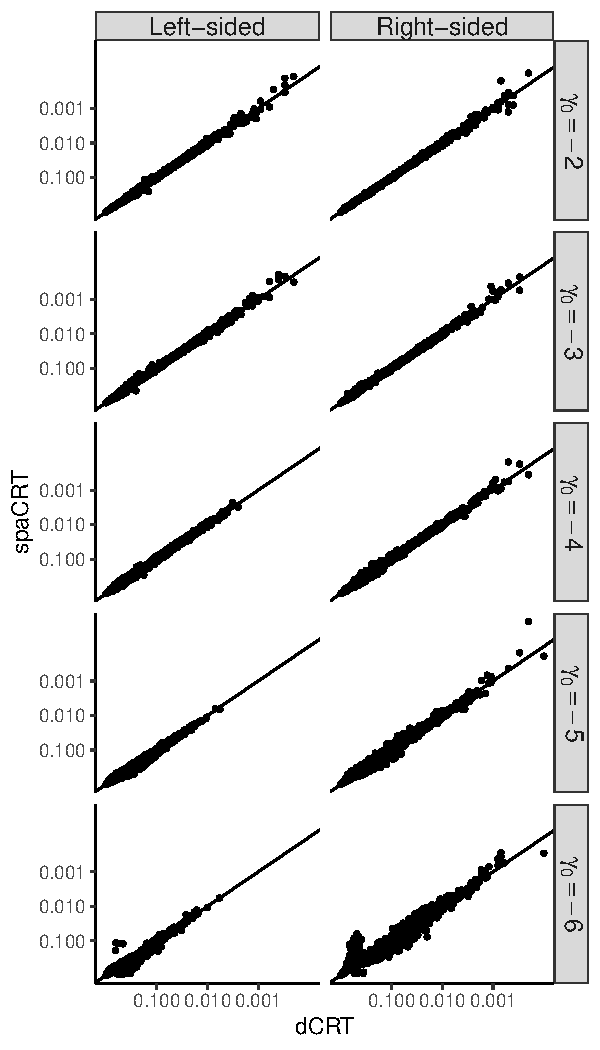
\includegraphics[width=0.7\textwidth]{figures-and-tables/simulation/NB-regression/QQ/disp-0.05-dCRT-spaCRT-varying-gamma.pdf}
  %   \caption{Scatter plots for the $p$-values of the left-sided and right-sided tests when varying $\gamma_0\in \{-6,-5,-4,-3,-2\}$ and fixing $\beta_0=-5$, with $r = 0.05$.}
  %   \label{fig:simulation-dot-plot-varying-gamma-theta-0.05}
  % \end{figure*}
  
  % \begin{figure*}
  %   \centering
  %   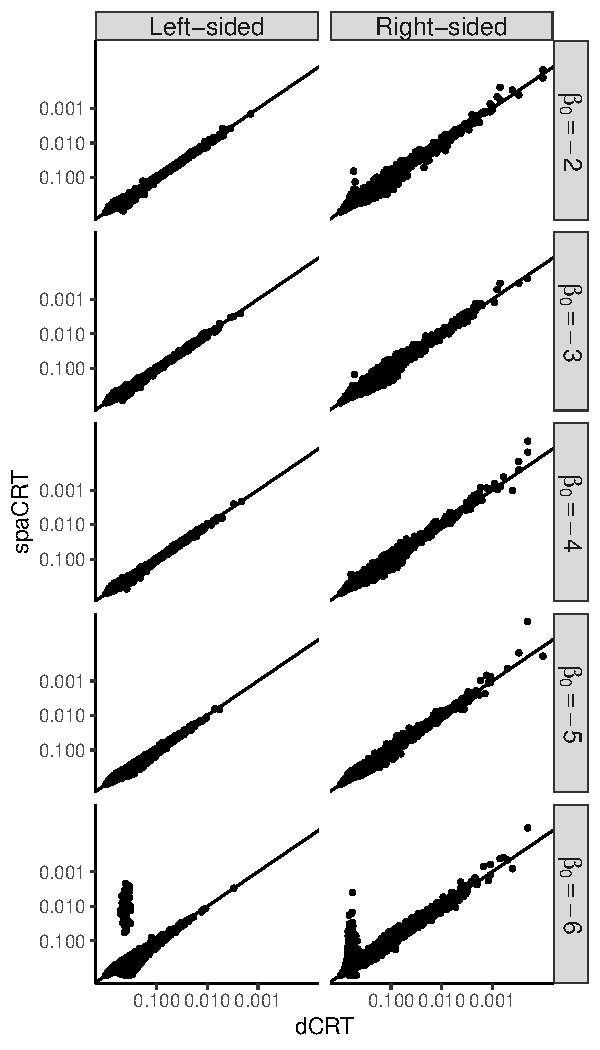
\includegraphics[width=0.7\textwidth]{figures-and-tables/simulation/NB-regression/QQ/disp-0.05-dCRT-spaCRT-varying-beta.pdf}
  %   \caption{Scatter plots for the $p$-values of the left-sided and right-sided tests when varying $\beta_0\in \{-6,-5,-4,-3,-2\}$ and fixing $\gamma_0=-5$, with $r = 0.05$.}
  %   \label{fig:simulation-dot-plot-varying-beta-theta-0.05}
  % \end{figure*}
  
  
  % \begin{figure*}
  %   \centering
  %   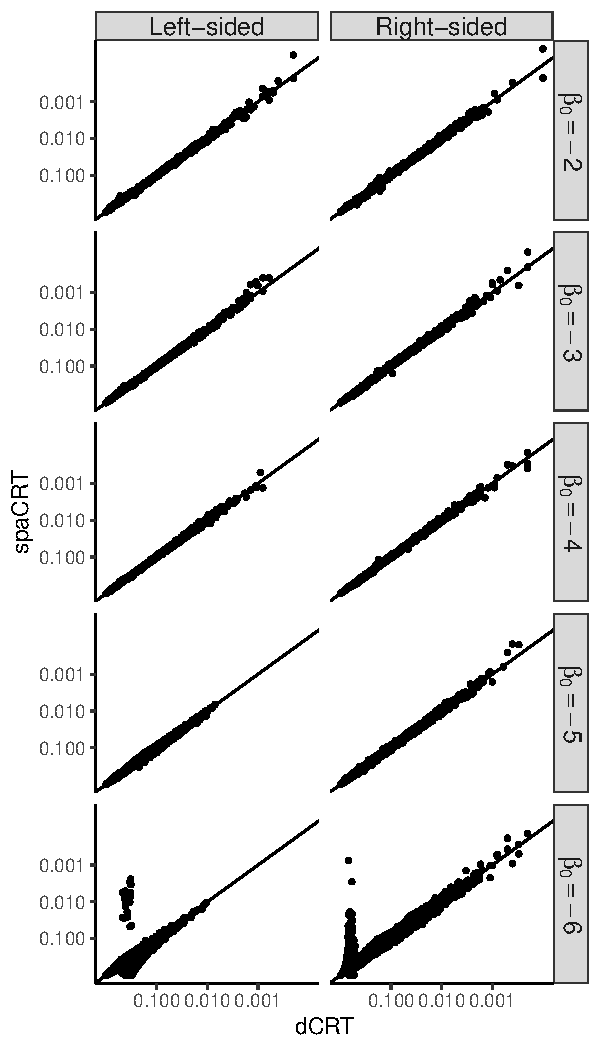
\includegraphics[width=0.7\textwidth]{figures-and-tables/simulation/NB-regression/QQ/disp-1-dCRT-spaCRT-varying-beta.pdf}
  %   \caption{Scatter plots for the $p$-values of the left-sided and right-sided tests when varying $\beta_0\in \{-6,-5,-4,-3,-2\}$ and fixing $\gamma_0=-5$, with $r = 1$.}
  %   \label{fig:simulation-dot-plot-varying-beta-theta-1}
  % \end{figure*}
  
  % \begin{figure*}
  %   \centering
  %   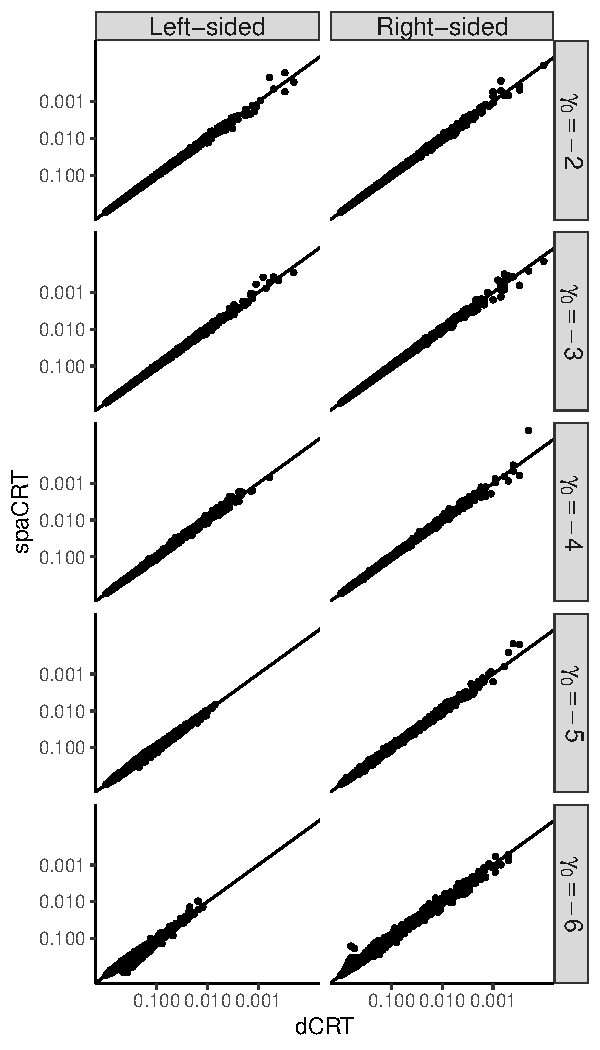
\includegraphics[width=0.7\textwidth]{figures-and-tables/simulation/NB-regression/QQ/disp-1-dCRT-spaCRT-varying-gamma.pdf}
  %   \caption{Scatter plots for the $p$-values of the left-sided and right-sided tests when varying $\gamma_0\in \{-6,-5,-4,-3,-2\}$ and fixing $\beta_0=-5$, with $r = 1$.}
  %   \label{fig:simulation-dot-plot-varying-gamma-theta-1}
  % \end{figure*}
  
  % \begin{figure*}
  %   \centering
  %   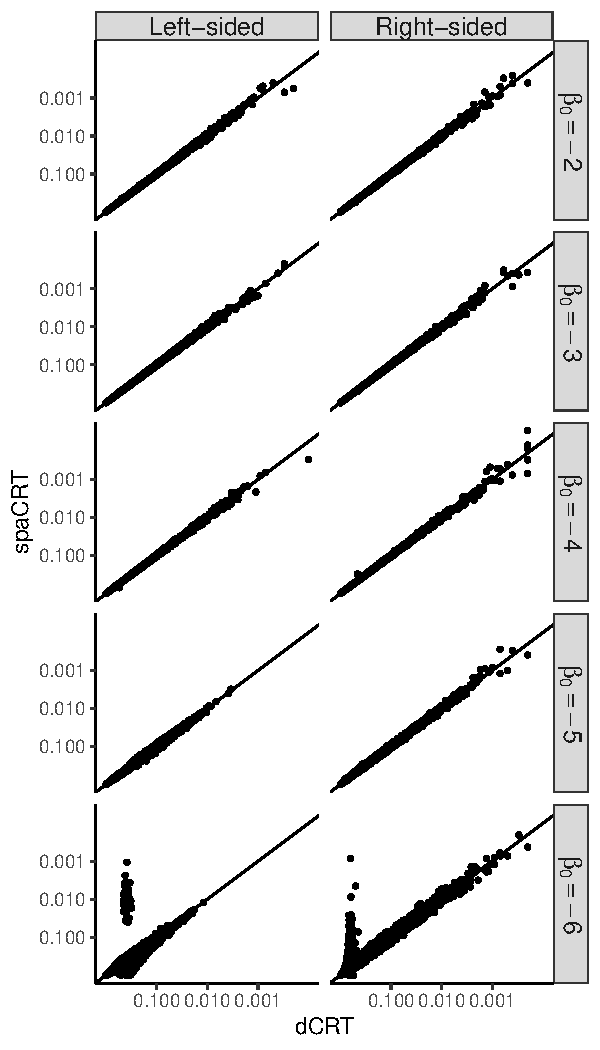
\includegraphics[width=0.7\textwidth]{figures-and-tables/simulation/NB-regression/QQ/disp-10-dCRT-spaCRT-varying-beta.pdf}
  %   \caption{Scatter plots for the $p$-values of the left-sided and right-sided tests when varying $\beta_0\in \{-6,-5,-4,-3,-2\}$ and fixing $\gamma_0=-5$, with $r = 10$.}
  %   \label{fig:simulation-dot-plot-varying-beta-theta-10}
  % \end{figure*}
  
  % \begin{figure*}
  %   \centering
  %   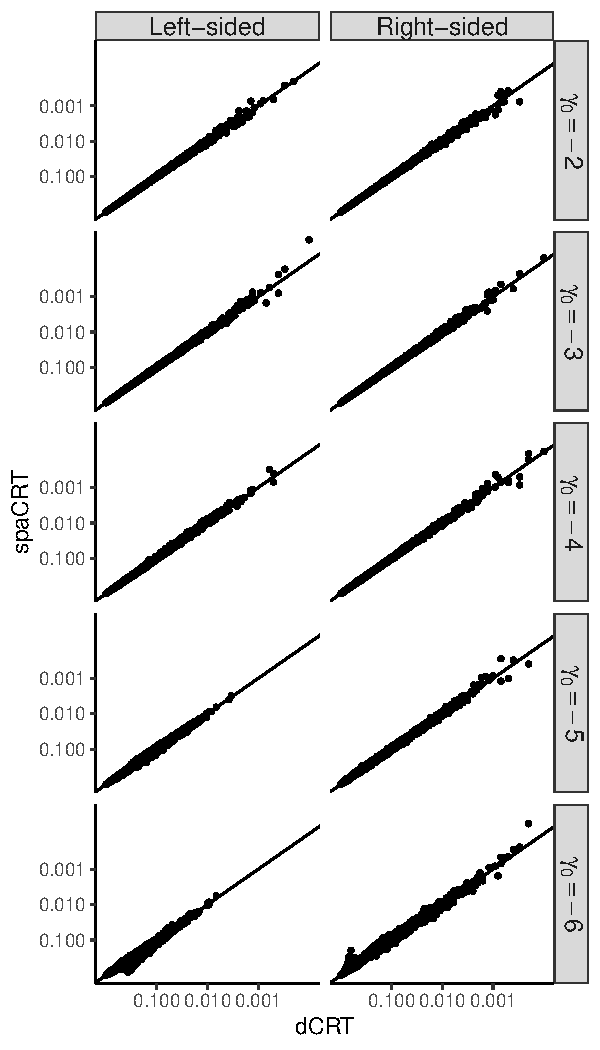
\includegraphics[width=0.7\textwidth]{figures-and-tables/simulation/NB-regression/QQ/disp-10-dCRT-spaCRT-varying-gamma.pdf}
  %   \caption{Scatter plots for the $p$-values of the left-sided and right-sided tests when varying $\gamma_0\in \{-6,-5,-4,-3,-2\}$ and fixing $\beta_0=-5$, with $r = 10$.}
  %   \label{fig:simulation-dot-plot-varying-gamma-theta-10}
  % \end{figure*}
  
  
  \begin{figure}[!ht]
    \centering
    \includegraphics[width=0.8\textwidth]{figures-and-tables/simulation/NB-regression/FDR/disp-0.05-multiple_testing_rejection_plot.pdf}
    \caption{Averaged number of rejections after BH and Bonferroni corrections under the setup $r=0.05$.}
    \label{fig:simulation-CRISPR-screens-high-multiplicity-disp-0.05}
  \end{figure}
  
  
\clearpage

\section{Additional simulation details in Section \ref{sec:GWAS}}\label{sec:additional_details_GWAS}



\subsection{Parameters and methods implementation in Section \ref{sec:GWAS}}\label{sec:simulation_methods_GWAS}

\paragraph{Parameters used in Section \ref{sec:GWAS}}
Recall the logistic regression model:
\begin{align*}
	\law(\pry|\prx)\overset{d}{=}\text{Ber}(\expit(\gamma_0 + \prx^\top \beta))
\end{align*}
where $\gamma_0$ is an intercept term, $\beta$ is a vector of coefficient and $g$ is a smooth function. For the concrete choice of $\beta$, we consider 
\begin{align*}
	\beta = (\underbrace{\eta,\ldots,\eta}_{0.05 * p},\underbrace{-\eta,\ldots,-\eta}_{0.05 * p},\underbrace{0,\ldots,0}_{0.9 * p})^\top
\end{align*}
where $\eta>0$ is a signal strength. We vary $\eta\in\{0, 0.25, 0.5, 0.75, 1\}$. For $\gamma_0$, we consider $\{-3,-2\}$ for \textit{high} and \textit{low} sparsity settings. For the distribution of $\prx$, we consider the mHHM (Definition \ref{def:mhhm}) where we set the support of the hidden variable $\pru_j$, $K$, to be $10$ and that of $\prx$, $M$, to be $2$. The Markov transition matrix is 
\begin{align*}
	Q\equiv 
	\begin{pmatrix}
		\gamma & 1-\gamma & 0 & \ldots & 0 & 0\\
		0 & \gamma & 1-\gamma & \ldots & 0 & 0\\
		\vdots & &  \ddots & & &\vdots\\
		\vdots & &  & \ddots & &\vdots\\
		0 & 0 & 0 & \ldots & \gamma & 1 - \gamma\\
		0 & 0 & 0 & \ldots & 0 & 1\\
	\end{pmatrix}
	\in\mathbb{R}^{K\times K}.
\end{align*}
We set $\gamma=0.9$ to create non-trivial correlation between $\prx_j$. The intial distribution $q$ is a uniform distribution over the support of $\pru_1$. Besides the transition matrix, we also vary the emission distribution $\prx_j|\pru_j$ by considering a beta-piror emission distribution:
\begin{align}\label{eq:beta_emission}
  \P[\prx_j=1|\pru_j=k]\overset{\mathrm{i.i.d.}}{\sim} \mathrm{Beta}(\alpha,\beta).
  \tag{beta-emission}
\end{align}
Hyperparameter $(\alpha,\beta)$ controls the shape of the Beta distribution. We consider two choices: $(\alpha,\beta)=(1,3)$ and $(\alpha,\beta)=(1,1)$. The first set of parameters will put more mass towards small values close to $0$, which induce high sparsity and thus mimic the rare genetic variation setup. The second choice is a uniform distribution over $[0,1]$ with no skewness. Thus this induce low sparsity in $X$ and thus mimic the common genetic variation scenario. The simulation setup can be summarized in Table \ref{tab:simulation_parameter_GWAS}.

\begin{table}[!ht]
  \centering
  \caption{\label{tab:simulation_parameter_GWAS}Parameters considered in GWAS simulation.}
  \centering
  \begin{tabular}[t]{cc}
  \toprule
  Parmeters $(\alpha,\beta,\gamma_0)$ & Sparsity level for $(X,Y)$\\
  \midrule
  $(1,3,-2)$ & (high, low) \\
  $(1,3,-3)$ & (high, high) \\
  $(1,1,-2)$ & (low, low) \\
  $(1,1,-3)$ & (low, high) \\
  \bottomrule
  \end{tabular}
\end{table}
\noindent We will consider regularization parameters $\lambda$ used in \texttt{glmnet} to be $\lambda=\texttt{lambda.1se}$ or $\lambda=\texttt{lambda.min}$. 


\paragraph{Methods details in Section \ref{sec:GWAS}}

We devote this section to discussing the computational details of each method and we will discuss a simple yet powerful computational trick to compute the leave-one-out conditional expectations $\widehat \E[\pry|\prx_{-j}]$ for $\dCRT,\spacrt$ and $\GCM$. We first observe the following identity:
\begin{align*}
	\E[\pry|\prx_{-j}]=\E[\E[\pry|\prx]|\prx_{-j}]
\end{align*}
where the outer expectation is taken with respect to the measure $\prx_j|\prx_{-j}$. If we can estimate the joint distribution of $\prx$ from data $X$ and one regression estimate for $\E[\pry|\prx]$, computing the conditional expectation $\E[\pry|\prx_{-j}]$ for any $j\in[p]$ is straightforward via the integral evaluation with respect to measure $\prx_j|\prx_{-j}$, without any additional regression fit. In other words, we only need one regression fit for $\E[\pry|\prx]$ and one joint distribution fit for $\prx$. In practice, we consider using the following algorithm:
\begin{enumerate}
  \item \textbf{Estimate distribution $\prx$:} this can be done by using \texttt{fastPhase} \citep{scheet2006fast};
  \item \textbf{Compute regression estimate $\widehat \E[\pry|\prx=x]$:} this can be done by using \texttt{glmnet} \citep{tibshirani1996regression} with the family set to be \texttt{binomial};
  \item \textbf{Compute $\widehat\E[\pry|\prx_{-j}]$ for any $j\in[d]$:} this can be done by computing the following integral:
  \begin{align*}
    \widehat\E[\pry|\prx_{-j}=x_{-j}]=\sum_{x_j\in\{0,1\}}\widehat\E[\pry|\prx=x]\widehat \P[\prx_j=x_j|\prx_{-j}=x_{-j}],
  \end{align*}
  where $\widehat{\P}[\prx_j=x_j|\prx_{-j}=\cdot]$ is estimated using the \texttt{fastPhase} algorithm.
\end{enumerate}


\subsection{Additional simulation results in Section \ref{sec:GWAS}}\label{sec:simulation_results_GWAS}

We present four simulation results with each corresponding to the choice of \texttt{lambda.min} or \texttt{l
ambda.1se} and the sparsity level in $X$. High sparsity in $X$ with \texttt{lambda.1se} has been presented in Figure \ref{fig:simulation-summary-GWAS-skew-lambda-1se}. The other three plots can be found in Figure~\ref{fig:simulation-summary-GWAS-uniform-lambda-1se},\ref{fig:simulation-summary-GWAS-uniform-lambda-min} and \ref{fig:simulation-summary-GWAS-skew-lambda-min}.

We want to point out that the choice of $\lambda$ seems to affect both the FDR and power of the methods. In particular, comparing Figure~\ref{fig:simulation-summary-GWAS-uniform-lambda-1se} and Figure~\ref{fig:simulation-summary-GWAS-uniform-lambda-min}, we can find the FDR can be slightly inflated when \texttt{lambda.min} is used for $\dCRT,\GCM$ and $\spacrt$ methods whereas the FDR is well controlled when \texttt{lambda.1se} is used. The inflation of false positive rate can be because of the tower trick used for these methods. The intuition is that when \texttt{lambda.1se} is used for $\dCRT,\GCM$ and $\spacrt$, the estimated regression coefficients are more sparse and the models obtained from \texttt{glmnet} is less variable whereas \texttt{lambda.min} will lead to more variable models due to the relatively dense model it will produce. On the power side, we can see that the power of $\dCRT,\GCM$ and $\spacrt$ is slightly improved when \texttt{lambda.min} is used. Interestingly, the FDR of Knockoff procedure seems to be more robust to the choice of $\lambda$ whereas the power is worse when \texttt{lambda.min} is used, which is different from the behavior of $\dCRT,\GCM$ and $\spacrt$. 

\begin{figure}[!ht]
  \centering
  \includegraphics[width=1.0\textwidth]{figures-and-tables/simulation/HMM-variable-selection/HMM_simulation_uniform_lambda.1se.pdf}
  \caption{Summary of numerical simulation results for variable selection  with low sparsity in data $X$. All the results are obtained with the regularization parameter $\lambda=\texttt{lambda.1se}$. (a) FDR for $\gamma_0=-3$ (high sparsity) and $\gamma_0=-2$ (low sparsity). (b) Power for the same set of $\gamma_0$. (c) Computation times consumed by different methods. }
  \label{fig:simulation-summary-GWAS-uniform-lambda-1se}
\end{figure}

\begin{figure}[!ht]
  \centering
  \includegraphics[width=1.0\textwidth]{figures-and-tables/simulation/HMM-variable-selection/HMM_simulation_uniform_lambda.min.pdf}
  \caption{Summary of numerical simulation results for variable selection  with low sparsity in data $X$. All the results are obtained with the regularization parameter $\lambda=\texttt{lambda.min}$. (a) FDR for $\gamma_0=-3$ (high sparsity) and $\gamma_0=-2$ (low sparsity). (b) Power for the same set of $\gamma_0$. (c) Computation times consumed by different methods. }
  \label{fig:simulation-summary-GWAS-uniform-lambda-min}
\end{figure}


\begin{figure}[!ht]
  \centering
  \includegraphics[width=1.0\textwidth]{figures-and-tables/simulation/HMM-variable-selection/HMM_simulation_skew_lambda.min.pdf}
  \caption{Summary of numerical simulation results for variable selection with high sparsity in data $X$. All the results are obtained with the regularization parameter $\lambda=\texttt{lambda.min}$. (a) FDR for $\gamma_0=-3$ (high sparsity) and $\gamma_0=-2$ (low sparsity). (b) Power for the same set of $\gamma_0$. (c) Computation times consumed by different methods. }
  \label{fig:simulation-summary-GWAS-skew-lambda-min}
\end{figure}

\clearpage

\section{Simulation on unbalanced nonparametric classification}\label{sec:nonparametric_RF_classification}



\newpage

\section{Additional figures and tables for real data anlaysis}

In section \ref{sec:additional_table_realdata}, we show a table including the number of rejections when applying Bonferroni or BH method to the pairs invlovling the non-targeting perturbations (thus under the null). The total number of hypotheses is $153000$. In section \ref{sec:additional_figure_realdata}, we present additional figures for real data analysis including QQ-plots faceting across different effective sample size (Figure \ref{fig:qqplot_lowess}) and QQ-plots faceting across different dispersion parameters (Figure \ref{fig:qqplot_dispersion}). 

\subsection{Additional tables for the real data analysis}\label{sec:additional_table_realdata}

\begin{table}[!h]
\centering
\caption{\label{tab:real_data_rejection}Number of rejections for negative control pairs on the Gasperini data.}
\centering
\begin{tabular}[t]{lrrrr}
\toprule
\multicolumn{1}{c}{ } & \multicolumn{4}{c}{Number of rejections} \\
\cmidrule(l{3pt}r{3pt}){2-5}
\multicolumn{1}{c}{ } & \multicolumn{2}{c}{Left-sided test} & \multicolumn{2}{c}{Right-sided test} \\
\cmidrule(l{3pt}r{3pt}){2-3} \cmidrule(l{3pt}r{3pt}){4-5}
\multicolumn{1}{c}{Method} & \multicolumn{1}{c}{Bonferroni} & \multicolumn{1}{c}{BH} & \multicolumn{1}{c}{Bonferroni} & \multicolumn{1}{c}{BH} \\
\cmidrule(l{3pt}r{3pt}){1-1} \cmidrule(l{3pt}r{3pt}){2-2} \cmidrule(l{3pt}r{3pt}){3-3} \cmidrule(l{3pt}r{3pt}){4-4} \cmidrule(l{3pt}r{3pt}){5-5}
GCM test & 22 & 128 & 0 & 0\\
Score test & 1 & 1 & 15 & 29\\
spaCRT & 1 & 1 & 0 & 0\\
dCRT & 1 & 4 & 0 & 0\\
\bottomrule
\end{tabular}
\end{table}



\subsection{Additional figures for the real data analysis}\label{sec:additional_figure_realdata}

\begin{figure*}[!ht]
	\centering
	\includegraphics[width=0.9\textwidth]{figures-and-tables/facet_plot_different_withglmnb_100.pdf}
	\caption{QQ-plots for the $p$-values of right-sided test from different methods under low effective sample size.}
	\label{fig:qqplot_lowess}
\end{figure*}

\begin{figure*}[!ht]
	\centering
	\includegraphics[width=0.9\textwidth]{figures-and-tables/facet_plot_different_withglmnb_dispersion.pdf}
	\caption{QQ-plots for the $p$-values of left-sided test from different methods stratified by dispersion parameter.}
	\label{fig:qqplot_dispersion}
\end{figure*}

\clearpage


\end{document}






















 




